
\documentclass[refcompress,eversion,noinfo]{ICTthesis}

\usepackage{tabularx}
\usepackage{longtable}
\usepackage{color}
\usepackage{colortbl}
\usepackage{graphicx}
\usepackage{subfigure}
\usepackage{amsmath, epsfig}
\usepackage{enumerate}
\usepackage{multirow}
\usepackage{amsfonts}
\usepackage{algorithm}
\usepackage{algorithmic}
\usepackage{amsmath}
%\usepackage[margin=1.1in]{geometry}

\graphicspath{{figures/}}
%\linespread{1.3}

\definecolor{bkcolor1}{gray}{0.95}
\definecolor{bkcolor2}{gray}{0.85}
\newcommand{\bkcommand}[1]{\colorbox{bkcolor1}{$\mathtt{\backslash}$\texttt{#1}}}
\newcommand{\textgraph}[1]{\raisebox{-1ex}{\includegraphics[width=1.5em]{#1}}}

\renewcommand{\algorithmicrequire}{\textbf{Input:}} 
\renewcommand{\algorithmicensure}{\textbf{Output:}}

\begin{document}
\ICTfrontmatter

\begin{abstract}

影响力最大化问题是在社交网络中选择$k$个种子以

\keywords{社会影响力, 小世界网络, 近似算法, 路由}

\end{abstract}

\begin{englishabstract}

Influence maximization is the problem of selecting $k$ nodes in a social network to maximize their influence spread.
The problem has been extensively studied but most work focuses on the submodular influence diffusion models.
In this paper, motivated by empirical evidences, we explore influence maximization in the non-submodular regime.
In particular, we study the general threshold model in which a fraction of nodes have non-submodular threshold
	functions, but their threshold functions are closely upper- and lower-bounded by some submodular
	functions (we call them $\varepsilon$-almost submodular).
We first show a strong hardness result: there is no $1/n^{\frac{\gamma}{c}}$ approximation for influence maximization (unless P = NP)
	for all networks with up to $n^{\gamma}$ $\varepsilon$-almost submodular nodes, where $\gamma$ in $(0,1)$ 
	and $c$ is parameter depending on $\varepsilon$.
We then provide constant approximation algorithms when the number of non-submodular nodes are constant.
Finally, we conduct experiments on a number of real-world datasets, and the results demonstrate that our approximation algorithms
	outperform other benchmark algorithms.

\englishkeywords{Social Influence, Small World Network, Approximation Algorithm, Routing}

\end{englishabstract}

\ICTmainmatter

\chapter{绪论}
二十一世纪互联网发展迅猛,人与人之间不再仅仅只能当面交流,电子邮件、电话和即时通讯软件让人们之间的沟通更迅捷。与此同时,社交网站也在兴起,积累了越来越多的用户。在社交网络中,信息传播得更快,在社交网络中的营销手段会比传统营销获得更大的收益,有一些相关学者开始关注社交网络中的信息传播现象。


\section{课题研究的背景与意义}
社交网络(Social network)是由许多节点构成的一种社会结构。节点通常是组织和个人,节点之间的连接代表社会个体之间的关系,经由这些社会关系,把从偶然相识的泛泛之交到紧密结合的家庭关系的各种人们或组织串连起来。“社交网络”的概念从心理学、社会学、人类学、数学、统计学、计算机科学等不同领域不断深化,形成了一套系统的理论、方法和技术。在21世纪,人们获取信息的途径不再局限于报纸、广播、电视和当面交谈,随着Facebook,Twitter和Weibo等社交工具的广泛应用,社交网络已经成为重要的信息传播工具。在社交网络上,人们通过添加好友和关注建立人与人之间的连接,通过发消息、短文章、分享连接进行交流。信息在社交网络上可以沿着人与人之间的连接很快传播,很多新闻、广告在社交网络上可以很快的覆盖到绝大多数用户,这相对于传统的媒体介质有很大的优势。在互联网时代,社交网络成为了重要的信息传播工具,利用社交网络进行产品或信息的推广是很有力的手段。在实际应用场景中,会有这样的案例,某公司准备发售一款新产品,想要在社交网络上做一些免费体验活动,希望免费体验的人可以把产品较好的口碑在朋友间扩散出去,最后达到产品推广的目的。随之产生了这样一个优化问题,给定了网络结构和信息传播的模型之后,如何选定k个人作为种子,使得这$k$个人最后影响的范围最大,这就是社会网络影响力最大化\cite{Kempe2003maximizing}。这个问题被证明是NP难的,而且因为社交网络的规模很大,暴力的枚举所有种子集合很不现实,设计高效的有近似比保证的算法是很有需求的。

社会网络影响力最大化在被Kempe, Kleinberg和Tardos\cite{Kempe2003maximizing}提出并公式化之后,已经在学术界引起了广泛的关注,近年来很多学者都在做相关研究,涉及到病毒营销、媒体广告和谣言传播等方向。很多学者提出了比较有效的算法\cite{Kempe2003maximizing,Leskovec2007celf,Chen2009efficient,chen2010sharpphard,tang2014newrrset},这些算法大部分是采用了独立级联(Independent Cascade)或者线性阈值(Linear Threshold)[1]的信息传播模型。在这两种传播模型下,影响力函数是次模(Submodular)的,这时候可以使用贪心策略得到1-1/e近似的算法。此外,在一个更一般的通用阈值(General Threshold)\cite{Kempe2003maximizing}传播模型下,每个用户的阈值函数(Threshold Function)不再是简单的把边的权值相加,而是一个集合函数。伯克利的学者Elchanan和Sebastien\cite{Mossel2007sub}证明了阈值函数是次模的时候整体的影响力函数也是次模的,也就意味着局部的次模性质会导致全局的影响力函数的次模性。

然而,在真实的社交网络中,非次模的影响力传播现象经常出现。Backstrom[6]研究了LiveJounral和DBLP两个大型的社交网络数据,他绘制了个体加入某个社区的意愿与她的已经加入该社区好友数量的关系图。论文的图中可以看到意愿曲线整体上是上凸的,但是在最开始几个点有明显的下移。杨洋[7]等人观测了另一个社交网络Flickr,他们主要观察人的情绪变化被他带有情绪的朋友的影响。他们指出人变快乐的可能性和已经快乐的好友数量是一个超线性关系,尤其是那些影响力比较大的朋友。这些结果都指出现有的基于独立级联或者线性阈值模型的算法在真实的社会网络种可能并不能使用。很多非次模的传播模型已经被证明很难近似,像谣言和疾病的传播,需要社交网络中的个体在被影响邻居的数量超过某个阈值的时候才会被影响,这种模型也是通用阈值模型的变种,被称作固定阈值模型(Fixed Threshold Model)。在固定阈值模型下,社交网络影响力最大化问题是NP-hard的,而且有很强的不可近似性[1]。与此同时,如果考虑寻找能达到给定影响力目标的最小种子集合问题,也就是社会影响力最小化种子集合问题,陈宁也证明了这个问题也很难被近似[8]。学者们倾向于相信是次模性质帮助我们在社会影响力最大化问题中找到了比较好的近似算法。但是我们可以使用次模性质到什么程度呢?如果影响力传播过程仅仅是稍微偏离了次模性质,那么是否还有可能仍然设计一个近似比足够好的算法呢?这些问题现在仍然是需要解决的。

与此同时,固定阈值模型下的问题还有一些仍未被探索,前面说到的影响力传播,实际上只关心最后影响的人的数量,而不关心传播的时间和步数。考虑给定种子和目标节点的情况下,在不知道整体网络结构时,如何才能通过影响最少的人而影响目标?其实可以规定一个时间片只能影响一个人,问题就变成了社会网络里面,在固定阈值模型下,从给定的种子到目标点需要经过多少步跳转或者多少个时间片。这就是从另一个角度来研究社会影响力,从影响力传播的时间而不是影响的范围。此外,这里研究的是路由现象,就像IP包在路由网络里转发一样,IP包只知道最后的目的地,并不知道每一步应该具体怎么转发,也不能在每一个路由器群发,只能一步一步的跳转。我们研究的就是在社交网络里面的路由现象,跟传统路由的区别有两个,一个是社交网络的结构,没有路由表;另一个是每个节点被影响的邻居超过一定阈值时才能被影响到。在文章里,称类似IP包跳转的现象为简单路由,把影响需要阈值的路由为复杂路由。

社交网络是一个小世界网络,人与人之间的最短路很短。二十世纪60年代,美国哈佛大学社会心理学家斯坦利·米尔格伦(Stanley Milgram)做了一个连锁信实验[9]。他将一些信件交给自愿的参加者,要求他们通过自己的熟人将信传到信封上指明的收信人手里,他发现,294封信件中有64封最终送到了目标人物手中。而在成功传递的信件中,平均只需要5次转发,就能够到达目标。也就是说,在社会网络中,任意两个人之间的“距离”是6。这就是所谓的“六度分隔”理论(Six Degrees of Separation)。尽管他的实验有不少缺陷,但这个现象引起了学界的注意。小世界网络就是对这种现象(也称为小世界现象)的数学描述。用数学中图论的语言来说,小世界网络就是一个由大量节点构成的图,其中任意两点之间的平均路径长度比节点数量小得多。除了社会网络以外,小世界网络的例子在生物学、物理学、计算机科学等领域也有出现。许多现实中的图可以由小世界网络作为模型。万维网、公路交通网、脑神经网络和基因网络都呈现小世界网络的特征。本文采用经典的Kleinberg网络[10],这是一个基于二维网格的小世界网络,网格的边被称为人与人之间的强链接,而同时每个节点会发出若干条随机的弱连接。Kleinberg指出当模型的参数α等于网格的维度时,贪心路由算法有很高的效率。这里的贪心路由算法是指在每一步,当前节点把消息传递给他的邻居里面距离目标节点曼哈顿距离最小的节点。这个路由算法的需要的跳转数也符合之前Milgram的实验结果,从理论上支持了小世界现象。Kleinberg进一步指出当模型的参数α不等于网格的维度时,所有的路由算法都不能很快地把信件送达到目标手中。本文关注的是小世界网络中复杂路由的速度,复杂路由每一步激活的过程就是固定阈值模型,也是通用阈值模型范畴下的子问题。


\section{国内外研究现状}
自从基于BoW的图像检索框架\cite{sivic2003video}被提出以来,国内外学者对BoW中的几何校验问题就从未终止。针对BoW框架的几何校验基本可以分为两类,即检索后校验和检索时校验。检索后校验是指在进行正常的BoW检索之后,基于查询图片和匹配图片中特征点的几何一致性,对检索结果进行重新排序。检索后校验只考虑匹配点的几何关系,并且一般情况下,后校验的算法时间复杂度较高,只能对初排序结果的top N进行几何校验。检索时校验是指在进行BoW检索过程中进行几何校验,所以这种方法会考虑每对特征点之间的几何一致性。这就要求必须在进行检索之前将一些额外的有关于几何关系的信息融入到BoW向量中或倒排表内。一般情况下,检索时校验不会进行非常严格的几何校验,但是具有较高的检索效率。

\cite{sivic2003video}使用了一种相对简单的几何校验方案,称为空间一致性(Spatial Consistency)校验。这种校验考虑每个匹配点(局部特征点或区域)最近邻的匹配情况。具有空间一致性的点其最近邻的匹配点也应该在同一块区域内。这种方法只考虑了特征点在图片中相对位置关系的一致性。可以看出空间一致性检验是一种后校验方案。

利用RANSAC算法进行空间校验可以得到最好的几何校验效果,因为它要求很高的几何变换的一致性。首先定义匹配点之间变换矩阵,一般会考虑平移、旋转和尺度变换;然后计算每对匹配点之间的变换矩阵,并基于RANSAC算法得到最优的变化矩阵;最后根据这个变换矩阵,测试每对匹配点,符合这个变换的的点对被称为“inliers”,“inliers”数决定图片最终的相似度。\cite{philbin2007object}基于上述思想提出了Fast Spatial Matching(FSM)算法。由于FSM也是一种后校验的算法,FSM具有较高的计算复杂度,并且只能对Top N的检索结果进行校验,不能保证高召回率。\cite{Zhong2015Fast}对FSM做出改进并提出Direct Spatial Matching(DSM)。DSM直接计算尺度的变换,相比于其他基于RANSAC的算法,DSM需要更少的校验时间。

由于后校验的方法计算复杂度高、低召回率等问题,检索时校验同样得到人们的关注。这其中最经典的方法是基于空间金字塔(Spatial Pyramid)的几何校验算法。\cite{lazebnik2006beyond}和\cite{Cao2010Spatial}都是基于某种规则将一副图像分成若干区域,然后为每个区域生成一个BoW向量,最后将这些BoW向量连接到一起生成整幅图像的BoW向量。\cite{Cao2010Spatial}提出Spatial Bag-of-Features是\cite{lazebnik2006beyond}中Spatial Pyramid Matching的一般形式并且Spatial Bag-of-Features可以处理目标的基本变换,例如平移、旋转和尺度变化等。

近些年,CNN(Convolutional Neural Networks)在计算机视觉领域取得了巨大的成功,例如图像分类\cite{krizhevsky2012imagenet}、目标检测\cite{Girshick2014Rich}\cite{girshick2015fast}\cite{ren2015faster}、人脸识别,也包括图像检索\cite{babenko2014neural}。对于图像检索问题,一般是使用训练好的模型(同时可能会在某些数据集上进行fine-tune)提取图片的全局特征(网络某一层的输出),然后进行相似度的计算并排序。不同于传统的BoW检索框架,基于CNN的检索框架不考虑图片的旋转和尺度变化,而完全依赖于模型的能力和大规模的训练数据。在实际检索场景下,图片旋转是常见问题。现有网络一般使用Max Pooling操作,可以一定程度上应对旋转问题。

可以看到,国际上对于图像检索中几何校验的研究正呈现百花齐放的状态,研究人员从不同角度对几何校验进行了多方面的研究,形成了不同的算法与思路,这也恰好说明了人们对于显著性区域检测这一课题还处于探索研究阶段,并没有形成最优的解决方案,还存在多方面的问题亟待解决。



\section{本文所做的工作}
本文针对目前检索框架(包括BoW检索框架和CNN检索框架)中存在的问题,在Word Spatial Arrangement(WSA)\cite{penatti2014visual}基础上做出改进,提出Region Property Arrangement(RSA)空间校验算法。并且训练了学习图片主方向的CNN网络Main Orientation Net来解决CNN检索框架中图片旋转的问题。主要工作与成果如下:

\begin{enumerate}
\item  通过对WSA和其他空间校验算法的深入研究,提出了RSA空间校验算法。RSA方法首次提出了Region Property Space(RPS)的概念,并将图片中的特征区域(interest region)映射为RPS中的一个点。传统的空间校验算法只考虑匹配点对之间尺度、角度的相对变化,而RSA可以分析一副图片所有特征区域属性的分布规律,并将这种分布编码到BoW向量中,可以在检索过程中完成几何校验。RSA算法可以显著提高BoW检索的性能,在Holidays、Paris和Oxford数据库上达到了state-of-the-art的检索性能,同时不会增加计算和存储的负担。
\item  通过对RPS中点的分布进行深入的研究,我们发现RPS中点的分布具有很强的规律性,这种规律性在图片位置空间(基于特征点在图片上出现的位置)所不具备的。通过分析,我们在RPS的基础上提出了Spatial Weighting(SpW)。SpW可以解决图像检索中的burstniess\cite{jegou2009burstiness}的问题。并且,基于RPS中点的分布特性,我们提出了计算RSA的快速算法,比暴力算法快2到3倍。
\item 为了应对图像检索中图片旋转的问题,我们提出了MONet(Main Orientation Net)。由于图片主方向包含了图片的语义信息,传统的方法无法得到(只能得到某个区域的梯度方向)。借助深度学习方案,MONet很好的解决了查询图像可以旋转的问题,提高的检索的准确率。
\end{enumerate}

\section{论文组织结构}
本文分为五章,主要结构和内容如下:

第一章首先阐述了显著几何校验的研究背景和意义,接着介绍了该方向的国内外研究现状以及存在的问题,最后概述了本文所做的工作和论文的组织结构。

第二章介绍显几何校验测的基础特征与算法,并分类探讨了目前国际上各类主流算法的思路与不足。基于此,制定了本文的研究思路与框架。

第三章介绍Region Similarity Arrangement和Spatial Weighting算法,并通过详细的实验对比,全面评测了该算法的性能。

第四章介绍 Main Orientation Net,并将该网络应用到BoW和CNN检索框架中,对算法性能进行了全面评估。

最后一章对全文进行了总结,同时展望未来的研究工作。


\chapter{小世界网络及影响力传播基础}
在本章中,首先介绍Kleinberg小世界网络模型和影响力传播模型,
然后介绍常见的影响力传播模型,
最后介绍了影响力最大化算法的相关工作。

\section{Kleinberg小世界模型}\label{sec:kleinberg}
Kleinberg的小世界模型是一个由$n$个节点的集合$V$生成的随机图。
$n$个节点分布在一个$\sqrt{n} \times \sqrt{n}$的二维网格上\cite{Kleinberg2000small},为了方便,
我们把网格的上边界和下边界连接起来,同时也把网格的左边界和右边界连接起来。
这样二维网格就变成了“环面”,网格中每个节点的位置都是对称的。
网格上两个节点$u$和$v$之间的曼哈顿距离(Manhattan distance)$|uv|$是
在网格上$u$到$v$的最短路径的长度。

这个随机图上有两种类型的边:{\it 强连接}和{\it 弱连接}。
强连接是任意两个曼哈顿距离不超过$p$的节点之间生成的无向边,这里$p \geq 1$是一个模型的常数。
弱连接指连接节点$u$和网格上可能相距较远的节点$v$之间的随机边。
每个节点$u$会有$q$条互相独立的弱连接边,$u$的第$i$条弱连接边以$v$为终点的概率
正比于$1/{|uv|}^\alpha$,$\alpha\geq 0$是小世界模型的参数。
我们用$1/{|uv|}^\alpha$乘以归一化因子$\mathcal{Z} = 1/\sum_{v\in V}|uv|^{-\alpha}$(在环形网格上,这个值对于任意的节点 $u\in V$都相等),这样就得到了弱连接的概率分布函数。
最初Kleinberg描述的网络模型\cite{Kleinberg2000small}中,$u$到$v$之间的弱连接被认为是有向边,这样的网络被称为{\it 有向Kleinberg小世界网络模型}。
而有些研究工作\cite{Ghasemiesfeh2013complex}中弱连接被认为是无向的,这样的网络被称为{\it 无向Kleinberg小世界网络模型}。
两个模型在本文中都被讨论了,在分析复杂传染病的传播时,我们为了和以前的工作保持一致,
采用无向Kleinberg小世界网络模型。
分析复杂传染病的路由时,我们使用有向Kleinberg小世界网络模型。

\section{影响力传播模型}
社交网络被定义为一个有向图$G=(V,E)$,其中$V$是所有节点的集合,代表着网络中的个体,$E\subseteq V \times V$是有向边的集合。
$E$是网络中的关注或者粉丝关系,每条边也会有权值,权值代表着两个人的关系密切程度或者影响程度。
因为$G$是有向图,对于一个节点$v$,我们用$N^+(v)$表示所有$v$指向的节点集合,用$N^-(v)$表示所有指向$v$的节点集合,也就是$v$的出邻居(out-neighbours)和入邻居(in-neighbours)集合。
网络中的节点都有两种状态:{\it 未激活}(inactive)和{\it 激活}(activated)。
节点可以从未感染状态转变为感染状态,但是不能反方向转变,例如不能从已感染的状态变成未感染状态。
传播的过程可以用离散的时间步骤$0,1,2,\ldots$来描述。
在社交网络模型下,影响力传播被定义为一些疾病、信息或者想法在社交网络中沿着用户之间的有向边进行扩散。
对于一次传播过程,初始状态节点都是未激活的,选定图中的一些节点,把他们的状态设定为激活。
然后每一个时间片,按照设定的传播模型逐渐去尝试激活图未激活中的节点。
如果当前时间片没有新的节点被激活为止,传播过程结束。
接下来本文介绍常见的影响力传播模型。


\subsection{独立级联模型}
\begin{figure}[h]
	\centering
	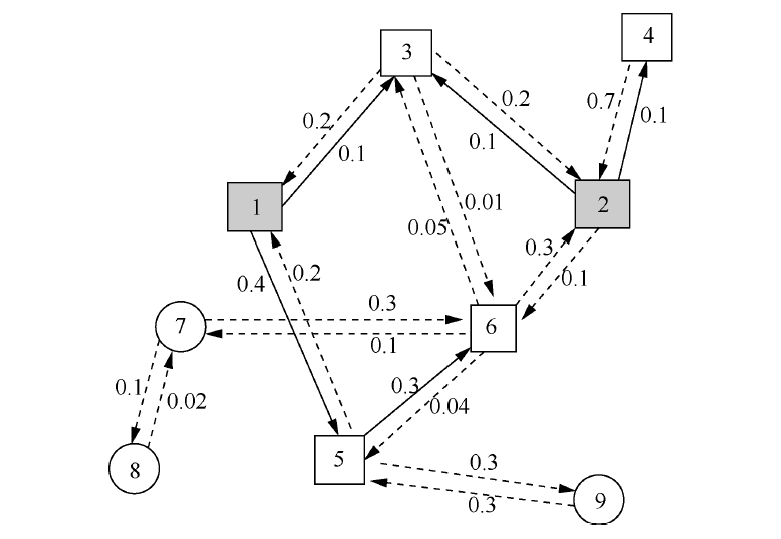
\includegraphics[width=\textwidth]{independent_cascade.png}
	\caption{独立级联模型示意}\label{fig:independent_cascade}
\end{figure}
独立级联模型(Independent Cascade Model)在03年被Kempe等人\cite{Kempe2003maximizing}提出,
在独立级联模型中,每条有向边$(u,v) \in E$都有一个概率值$p(u,v) \in [0,1]$代表着$v$被$u$影响的概率。
传播是随着离散时间片$t$增加而扩散的,定义$S_t$为到时间片$t$时刻为止被激活的节点的集合,定义$S_{-1}=\emptyset$。
在$t=0$时刻,选定$k$个节点$S_0$作为种子并把他们置为激活状态。
对于任意的$t\geq 1$时刻,每一个在$t-1$时刻激活的节点$v \in S_{t-1} \setminus S_{t-2}$都会对其所指向的未激活节点
$u \in N^+(u) \setminus S_{t}$进行一次激活尝试,成功激活$u$的概率是$p(v,u)$,不同节点之间的激活尝试相互独立。
如果节点$u$在某次激活尝试中被激活,则$u$在$t$时刻被激活。
如果$S_{t-1} \setminus S_{t-2}$中所有节点对$u$的尝试都失败,则$u$在$t$时刻未被激活。
当某一时刻没有节点被激活时,传播终止。

图\ref{fig:independent_cascade}给出了独立级联模型下的一次传播过程,图中的虚线边表示一次失败的激活尝试,实线表示成功的激活尝试。
在$t=0$时刻节点1和节点2被选为种子,在$t=1$的时刻,节点1和节点2成功激活了节点3、4、5,节点2对节点6的激活尝试失败。
在$t=2$时刻节点5成功激活了节点6,节点3和4发出的尝试激活失败。
在$t=3$时刻节点6没有激活任何节点,传播过程终止,最后被影响的节点集合是$\{1,2,3,4,5,6\}$。

\subsection{线性阈值模型}
独立级联模型(Linear Threshold Model)\cite{Kempe2003maximizing}描述的传播过程中,节点对节点的作用是互相独立的,而且每个节点只需要一次成功的激活尝试就能被激活。
而在有些场景中,一个节点的激活需要多个节点的共同作用,像购物或者接受新商品等。
为了描述类似举要多个节点累计作用才能激活的场景,线性阈值模型被提出来。

在现行与之模型中,每条有向边$(u,v) \in E$都被赋予了一个权重$w(u,v)$,对于每个节点来说,所有指向它的边权重之和不超过$1$。
也就是$\sum_{u \in N^-(u)} w(u,v) \leq 1$。
每个节点$v$还有自己的阈值$\theta_v \in [0,1]$,在传播开始前,每个节点独立的在$[0,1]$中依据均匀分布选择自己的阈值。
在每个时间节点$t \geq 1$,对于所有还没被激活的节点$v \in V \setminus S_{t-1}$,
如果由已激活节点发出的指向$v$的的有向边权重之和大于$v$的阈值,也就是$\sum_{u \in N^-(u) \cap S_{t-1}} w(u,v) \geq \theta_v$,
则$v$会在$t$时刻被激活,否则停留在未激活状态。
同样,当在某一时刻没有新节点被激活时,传播停止。

\subsection{通用级联模型}
独立级联模型的假设过强,于是Kempe\cite{Kempe2003maximizing}提出了通用级联模型(General Cascade Model),
这是独立级联模型的一般形式。
对于通用级联模型,每个节点$v$有个激活函数$p_v(u,S):N^-(v) \times 2^{N^-(v)} \to [0,1]$,
这里$S \subset N^-(v)$并且$u \in N^-(v) \setminus S$。
传播过程整体和独立级联模型一致,
在$t=0$时刻选定种子节点后,在$t \geq 1$的时间片,
对于尚未激活的节点$v \not\in S_{t-1}$,把$v$刚刚激活的的入邻居$N^-(v) \cap (S_{t-1}\setminus S_{t-2})$按照$u_1,u_2,\dots,u_{\ell}$排列,
依据这个顺序依次尝试激活节点$v$。
如果$u_1,u_2,\dots,u_{i-1}$没有成功激活$v$,则令$S = (N^-(v) \cap S_{t-2}) \cup \{u_1,u_2,\dots,u_{i-1}\}$
然后$u_{i}$以$p_v(u_i,S)$的概率尝试激活$v$。
在通用级联模型中,$p_v(u,S)$满足顺序无关性质,也就是最终$u_1,u_2,\dots,u_{\ell}$尝试激活$v$之后$v$被激活的概率
与这$\ell$次尝试的顺序无关,只与尝试激活的节点集合有关。
注意到独立级联模型是通用级联模型的特例,只需要令$p_v(u,S)$恒等于$p(u,v)$即可。


\subsection{通用阈值模型}
在通用阈值模型中(General Threshold Model),每个节点$v$有一个阈值函数$f_v:2^{N^-(v)} \to [0,1]$。
阈值函数$f_v$是单调非减(monotone)而且$f_v(\emptyset)=0$。
和线性阈值模型相同,在传播开始前,每个节点独立的在$[0,1]$中依据均匀分布选择自己的阈值。
然后在接下来的每一时刻$t\geq 1$,对于$v \not\in S_{t-1}$,
如果$f_v(S_{t-1} \cap N^-(v)) \geq \theta_v$,
节点$v$被激活,否则节点$v$保持未激活状态。

%线性阈值模型是通用阈值模型的特例,只需要令$f_v(S) = \sum_{u\in S}w(u,v)$。
通用阈值模型和通用级联模型也是等价的,给定阈值函数$f_v$,可以得到激活函数
$p_v(u,S) = \frac{f_v(S \cup \{u\}) - f_v(S)}{1-f_v(S)}$。
给定激活函数$p_v$,同样可以得到对应的通用阈值模型的阈值函数
$f_v(S) = 1 - \Pi_{i=1}^{\ell}(1-p_v(u_i, \{u_1,u_2,\dots,u_{i-1}\}))$。


\section{影响力最大化问题}
在一个$n$个节点的图中,给定影响力传播模型,最多经过$n-1$步,传播就会结束。
我们称以$S_0$为种子集合最终传播停止时被影响的节点集合是$\Phi(S_0)$。
$\Phi(S_0)$是一个依赖于影响力传播过程的随机集合。
影响力最大化问题就是在给定种子数量选择合适的种子集合的情况下最大化$\Phi(S_0)$的期望大小。
我们定义$\sigma(S_0) = \mathbb{E}(\Phi(S_0))$,$\sigma(\cdot)$就被称作为{\it 影响力函数}。
通常所研究的种子集合大小不超过$k$的影响力最大化问题可以公式化为$S^* = \mathrm{argmax}_{S \in V, |S|=k} \sigma(S)$,
$S^*$为最优解集合。
通常选用的影响力模型是独立级联模型或者线性阈值模型,近些年来也有很多基于这两个传播模型的影响力最大化算法被提出。

影响力最大化本质上描述了社交网络中的营销(Social marketing)问题,
有新的产品或者广告发布时,希望选择人试用并转发消息,然后口口相传最后扩散到很多人。
商家最后的目的就是希望可以遭到影响力最大的用户集合使得最终扩散的范围最大,这也就是影响力最大化的目标。
影响力最大化问题是社交网络中营销问题的抽象,研究影响力最大化问题对于商家试用品和广告的投放有很大帮助。
下面介绍一下影响力最大化问题的常见算法。

\subsection{贪心算法}
影响力最大化问题的复杂度很高,至少比集合覆盖最大化(Max Set Cover)问题要难,而集合覆盖最大化问题是NP-Hard的。
但是影响力函数$\sigma(\cdot)$在独立级联模型和线性阈值模型下被证明是次模的\cite{Kempe2003maximizing}。
次模函数是定义在集合函数上的,对于一个集合函数$f:2^V \to \mathbb{R}$,
如果对于任意的输入集合$S \subseteq T \subseteq V$和元素$u \in V \setminus T$都有
$f(S \cup \{u\}) - f(S) \geq f(T \cup \{u\}) - f(T)$,
则称函数$f$满足次模(submodular)性质。
次模性质本质上是边际效益递减,同样加入一个元素$u$,$f(T)$函数值的提升不如$f(S)$的提升大。
如果对于输入$S \subseteq T \subseteq V$,$f$函数还满足$f(S) \leq f(T)$,则称函数$f$是单调非减的。
对于单调非减和次模的函数$f$,贪心算法可以做到$1-\frac{1}{e}$的近似比。
对于影响力最大化问题,由于影响力函数$\sigma(\cdot)$是单调和次模的,可以调用贪心算法解决。
然而每一步$\sigma(S)$的计算是$\#$P-Hard的,不能精确求解。
通常采用蒙特卡洛模拟方法来估算影响力,随机模拟10000次传播过程,取被激活节点个数的期望作为影响力。
由于蒙特卡罗模拟是近似得到影响力大小,贪心算法最后可以取得$1-\frac{1}{e}-\varepsilon$的近似比。
蒙特卡洛贪心算法执行过程如Algorithm \ref{alg:mc_greed}所示。

\begin{algorithm}[h]
	\caption{\textbf{MC-Greedy(G,k)}: Monte Carlo greedy for influence maximization.}
	\label{alg:mc_greed} 
	\begin{algorithmic}[1]
		\Require $G$: social graph of IC or LT model, $k$: budget of seeds.
		\Ensure selected seed set $S$.
		\State Initialize $S = \emptyset$
		\For {$i=1$ to $k$}
			\State $v = \mathrm{argmax}_{u \in V \setminus S}$ \Call{MC-Spread}{$S \cup \{u\}, G$}
			\State $S = S \cup \{u\}$
		\EndFor
		\State \Return $S$
		\Function{MC-Spread}{$S$, $G$}
			\State $count=0$
			\For {$j=1$ to $R$}
				\State simulate diffusion process on graph $G$ with seed set $S$
				\State $n\_spread \gets$ the number of active nodes
				\State $count = count + n\_spread$
			\EndFor
			\State \Return $count/R$
		\EndFunction
	\end{algorithmic} 
\end{algorithm}

\subsection{CELF算法}
暴力的贪心算法时间复杂度很高,对于$k$个种子的影响力最大化问题,需要迭代$k$轮,每一轮需要便利每一个种子,利用蒙特卡洛模拟估计影响力大小。
最终需要的时间复杂度为$O(Rknm)$,$R$是蒙特卡洛模拟需要的传播模拟次数。对于几万个节点的图,贪心算法的运行时间可能就需要几周。
Leskovec等人\cite{Leskovec2007celf}基于次模问题优化中的lazy evaluation方法,优化了暴力的贪心算法,得到了近700倍的算法性能提升。
定义函数的差分为$\Delta_u f(S) = f(S \cup \{u\}) - f(S)$,其中$u \not\int S$。
对于单调次模函数$f$和集合$S \subseteq T \subseteq V$来说,有$\Delta_u f(S) \geq \Delta_u f(T)$。
在蒙特卡洛贪心算法中,每一轮都需要计算每个节点$v$的$\Delta_v f(S)$然后选出提升最大的节点加入$S$。
设$S_i$为第$i$轮为止选择到的种子节点集合,如果在第$i$轮算法运行中,发现存在节点$u,v \not\in S_{i-1}$,而且$\Delta_u f(S_{i-2}) \leq \Delta_v f(S_{i-1})$。
那么由次模性质可以得到$u$在第$i$轮的提升一定会小于$v$,所以不会被选为种子,在第$i$轮$u$的影响力提升就没有必要再计算。
所以加入一个结构存储之前计算的影响力提升,可以减少对影响力的重复估算,极大提升算法效率。
CELF算法就是利用这个思想,通过优先队列实现。

\begin{algorithm}[h]
	\caption{\textbf{CELF(G,k)}: accelerated greedy algorithm with lazy evaluation.}
	\label{alg:celf} 
	\begin{algorithmic}[1]
		\Require $G$: social graph of IC or LT model, $k$: budget of seeds.
		\Ensure selected seed set $S$.
		\State Initialize $S = \emptyset$, priority queue $Q = \emptyset$
		\ForAll {$v$ in V}
			\State $v.margin \gets$ \Call{MC-Spread}{$\{v\}, G$}
			\State $v.iteration = 1$
			\State insert element $v$ into $Q$ with $v.margin$ as the key
		\EndFor
		\State $iteration = 1, spread = 0$
		\While{$iteration \leq k$}
			\State extract top (max) element $v$ of $Q$
			\If{$v.iteration == iteration$}
				\State $S = S \cup \{u\}$
				\State $iteration = iteration+1$
				\State $spread = spread + v.margin$
			\Else
				\State $v.margin \gets$ \Call{MC-Spread}{$S \cup \{v\}, G$} - $spread$
				\State re-insert $v$ into $Q$
			\EndIf
		\EndWhile
		\State \Return $S$
	\end{algorithmic} 
\end{algorithm}

\subsection{PMIA算法}
MC-Greedy算法和CELF算法还是通过蒙特卡洛模拟来估算集合的影响力大小。陈卫等人提出了一个启发式算法,近似的估算影响力,再次提升了算法的性能,同时算法的效果能够媲美贪心算法。
PMIA算法\cite{chen2010sharpphard}中,利用比较容易计算的树状图来避免了蒙特卡洛模拟。
核心子算法是Maximum Influence Arborescence(MIA),PMIA算法对于每一个节点$v$构建了以$v$为根的局部树状结构,
然后在局部的树状结构上可以用动态规划高效计算影响力。
因为影响力传播衰减很快,而且估算整体的影响力很难,局部树状结构也是合理的。
PMIA算法同时也根据树状结构设计了线性更新影响力提升值的方法,在加入新的种子节点后很快更新每个节点的影响力。
原算法的整体过程比较复杂,由多个子算法构成,这里不再赘述。

\subsection{TIM算法}
基于蒙特卡洛模拟的贪心算法速度较慢,启发式算法速度较快但是没有理论的近似比保证。
Borgs等人\cite{borgs2014rrset}在14年提出了基于逆向可达集合(Reverse Reachable Set)的近线性算法,同时也有基于最大集合覆盖的$1-\frac{1}{e}$的近似比保证。
算法的核心思想是做逆向蒙特卡洛模拟,把图中每条有向边反向,沿着反向的边做传播。
算法会随机的选择图中的节点$v$,然后以$v$为根节点做反向蒙特卡洛模拟,传播过程中激活的节点称为$v$的逆向可达集合,多次模拟得到多个逆向可达集合。
Borgs等人证明了,给定种子集合$S$,$v$被激活的概率就是$S$和$v$的逆向可达集合有交集的概率。
因此可以随机从途中选择节点,产生逆向可达集合,多次实验之后生成很多逆向可达集合。
给定一个种子集合,影响力大小正比于种子集合与多少个多逆向可达集合有交集,这就转变为最大集合覆盖问题,可以用贪心很快求解。
随后Tang等人\cite{tang2014newrrset}工程上实现了这个算法(TIM算法),并测试了算法在上亿节点的效果和运行时间。该算法已经能处理Twitter这种级别的社交网络。
在求解最大覆盖问题时,依据逆向可达集合简历倒排索引,维护每个节点覆盖的逆向可达集合,每次贪心的选择覆盖最多逆向可达集合的节点加入种子节点。

\begin{algorithm}[h]
	\caption{\textbf{TIM(G,k)}: Two-phase Influence Maximization.}
	\label{alg:tim} 
	\begin{algorithmic}[1]
		\Require $G$: social graph of IC or LT model, $k$: budget of seeds.
		\Ensure selected seed set $S$.
		\State Initialize $S = \emptyset$, $\mathcal{R} = \emptyset$
		\State compute the the number of RRsets needed $\theta$
		\For {$i=1$ to $\theta$}
			\State randomly pick a node $v$ from $V$
			\State generate RRset $R_v$ for $v$
			\State insert $R_v$ into $\mathcal{R}$
		\EndFor
		\State build reverse index $Idx$ of $\mathcal{R}$
		\For {$i=1$ to $k$}
			\State fetch $v$ that has max degree from $Idx$
			\State insert $v$ into $S$
			\State update $Idx$
		\EndFor
		\State \Return $S$
	\end{algorithmic} 
\end{algorithm}

\section{本章小结}
本章主要介绍了本文使用的Kleinberg小世界模型以及影响力传播模型和影响力最大化算法等概念,并给出了精确的数学定义。
2.1节介绍了Kleinberg的小世界模型,主要分析了弱连接的生成方式。
2.2节介绍了影响力传播模型,重点介绍了线性阈值模型和独立级联模型以及他们的通用形式。
2.3节介绍了基于线性阈值模型或者独立级联模型和影响力最大化,影响力最大化算法在近些年来被许多学者研究,很多近似算法和启发式算法被提出。



%
\chapter{Region Similarity Arrangement}
\section{引言}
按照上一章中制定的研究框架,本章介绍Region Similarity Arrangement(RSA)空间校验算法。首先,对本章工作的研究背景和相关工作进行了介绍,重点介绍了Spatial Coding\cite{zhou2010spatial}和Words Spatial Arrangement\cite{penatti2014visual}存在的问题。然后,逐步介绍RSA算法,包括Region Property Space(RPS),RPS中点的分布特性,如何构建RSA向量和快速计算RSA的算法;为了解决RSA在检索过程中存在的burstiness\cite{jegou2009burstiness}问题,接下我们来提出了Spatial Weighting;最后我们设计了基于RSA空间校验算法的大规模图像检索框架。实验结果表明RSA适用于大规模图像检索场景。

\subsection{相关工作介绍}
本文所提出的RSA几何校验方法与传统的基于点对之间的局部几何校验算法\cite{jegou2008hamming}\cite{philbin2007object}不同,RSA识图寻找某个特征点在一张图片中全局的几何关系。这种全局的几何校验算法有更加鲁棒,对尺度变化不敏感的特点。首先,我们先介绍两个同样考虑图片全局几何关系的算法,Spatial Coding(SC)\cite{zhou2010spatial}和Word Spatial Arrangement(WSA)\cite{penatti2014visual}。

\subsubsection{Spatial Coding}
\begin{figure}[h]
	\centering
	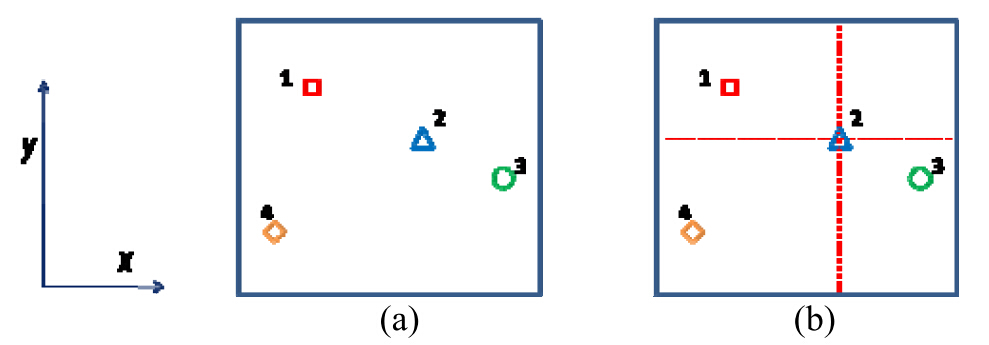
\includegraphics[width=\textwidth]{spatial_coding.jpg}
	\caption{计算$X$-map和$Y$-map示意图}\label{fig:sc}
\end{figure}
SC编码图片中每对特征点之间的相对位置关系。为了编码这种关系,SC会为每张图片生成两个空间图,称为$X$-map和$Y$-map。$X$-map编码了竖直方向上的点的相对位置关系,而$Y$-map编码了水平方向上点的相对位置关系。假设一张图片$I$有$K$个特征点$\{v_i\}$,则$I$的$X$-map和$Y$-map都是$K \times K$大小的二进制矩阵,其定义为:
\begin{equation}
X_{map}(i,j)=
\begin{cases}
0 & \text{if $x_i < x_j$} \\
1 & \text{otherwise}
\end{cases}
\end{equation}
\begin{equation}
Y_{map}(i,j)=
\begin{cases}
0 & \text{if $y_i < y_j$} \\
1 & \text{otherwise}
\end{cases}
\end{equation}
其中$(x_i,y_i)$和$(x_j,y_j)$是$v_i$和$v_j$的坐标(在图片的直角坐标系中)。图\ref{fig:sc}为计算$X$-map和$Y$-map的示意图,根据图中的例子得到的$X$-map和$Y$-map分别为:
\begin{equation}
X_{map}=
\left(
\begin{array}{cccc}
1 & 0 & 0 & 1 \\
1 & 1 & 0 & 1 \\
1 & 1 & 1 & 1 \\
0 & 0 & 0 & 1 \\
\end{array}
\right)
\end{equation}

\begin{equation}
Y_{map}=
\left(
\begin{array}{cccc}
1 & 1 & 1 & 1 \\
0 & 1 & 1 & 1 \\
0 & 0 & 1 & 1 \\
0 & 0 & 0 & 1 \\
\end{array}
\right)
\end{equation}

在得到$X$-map和$Y$-map之后就是如何使用它们进行几何校验。在检索时,对匹配的特征点进行SC校验。首先得到查询图像$I_q$和数据库图像$I_m$的SC子图$(GX_q,GY_q)$和$(GX_m,GY_m)$,然后对相应的子图进行异或操作,即:
\begin{equation}
V_x(i,j)=GX_1(i,j)\otimes GX_m(i,j)
\end{equation}
\begin{equation}
V_y(i,j)=GY_1(i,j)\otimes GY_m(i,j)
\end{equation}
异或结果中的‘1’表示不一致状态,这些不一致的总和越低两张图片的几何一致性越高,即几何一致性得分可以表示为:
\begin{equation}
S(I_q,I_m)=-\sum_{i=1}^{N}\sum_{j=1}^{N}V_x(i,j) - \sum_{i=1}^{N}\sum_{j=1}^{N}V_y(i,j)
\end{equation}


\subsubsection{Word Spatial Arrangement}
\begin{figure}[h]
	\centering
	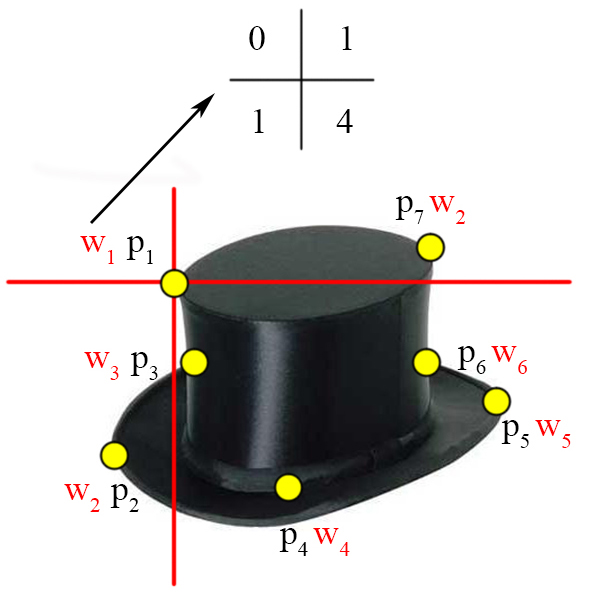
\includegraphics[width=0.5\textwidth]{WSA.jpg}
	\caption{计算WSA向量示意图}\label{fig:wsa}
\end{figure}
WSA提出了一种将特征点的相对位置关系编码到BoW向量中的算法,并在检索时校验特征点之间的几何一致性,所以WSA是一种检索时校验算法。图\ref{fig:wsa}为计算点$p_1$的WSA向量的示意图。计算WSA向量的具体算法如下:
\begin{enumerate}
	\item 将某个特征点(例如$p_1$)作为原点,建立直角坐标系,将图片分成四个象限;
	\item 统计四个象限内特征点的数目;
	\item 将这四个值进行L1归一化作为原点特征点的WSA向量;
	\item 重复上述步骤,求出图片中所有特征点的WSA向量。
\end{enumerate}

在进行检索时,对于具有相同视觉单词的点对,将他们对应WSA向量的直方图相交的值作为几何校验结果。WSA算法具有以下优点:
\begin{enumerate}
	\item 将特征点的几何关系编码到BoW向量中,在检索时进行几何校验,无需后处理,校验速度快;
	\item WSA编码特征点之间的相对位置关系,鲁棒性好;
	\item WSA可以与软量化\cite{philbin2008lost}算法结合使用。
\end{enumerate}

\subsection{现有方法的不足}
\begin{figure}[h]
	\centering
	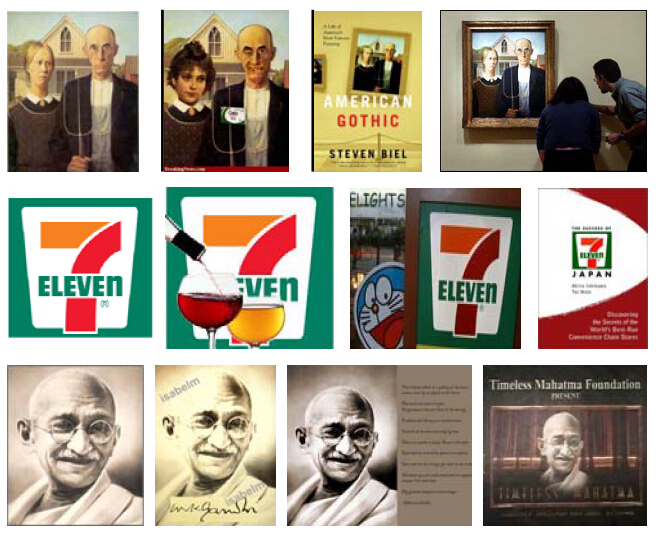
\includegraphics[width=0.7\textwidth]{sc_exa.jpg}
	\caption{部分重复(partially duplicated)相似图片}\label{fig:sce}
\end{figure}
\begin{figure}[h]
	\centering
	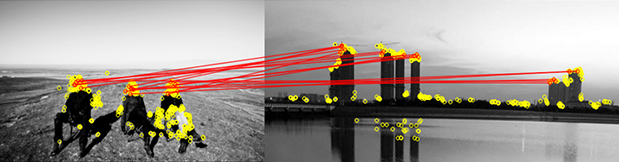
\includegraphics[width=0.8\textwidth]{WSA_exa.jpg}
	\caption{使用WSA算法后非相似图片之间特征点的匹配情况}\label{fig:wsae}
\end{figure}
以上方法虽然在某些情况下可以达到较好的校验算法,但依然存在一些问题:
\begin{enumerate}
	\item  SC几何校验算法通过二进制图编码了特征点之间严格的次序关系,这种校验算法要求图片之间有很强的相似性,甚至是在图片之间有完全一致的区域(如图\ref{fig:sce})才有比较好的效果。SC无法很好的应对更加一般的相似图像检索情况,尤其是视角、平移变化将导致二进制图较大的变化;
	\item WSA算法编码了特征点之间的相对位置关系。相比于SC,WSA算法更加鲁棒,适用于一般的检索问题。但是,图像中特征点的位置关系区分性低,无法进行较严格的几何关系校验。图\ref{fig:wsae}表明了即使考虑特征点之间的相对位置关系,还是会导致非相似图片之间的无匹配。
\end{enumerate}

本文提出的RSA算法试图解决上述问题,在完成较为严格的几何校验的同时达到一定的鲁棒性。除此之外,RSA还具有低内存消耗,低计算复杂度的特点,适用于大规模相似图像检索场景。

\section{Region Property Space}
在相似图像检索过程中提取特征的阶段,一块邻接的像素用来表述一个特征区域\cite{tuytelaars2008local},而这块区域通常用角度(angle)和尺度(scale)来描述。scale描述了这块区域覆盖的范围,而angle描述了这块区域的主方向(一般为梯度方向)。RSA将这两种属性编码到BoW向量中,并在检索时进行几何校验。因此,RSA算法需要解决两个问题:
\begin{enumerate}
	\item 如何编码视觉单词的属性信息(即angle和scale);
	\item 如何度量特征区域之间的相似性,并度量图像之间的相似性。
\end{enumerate}
第一个问题将通过本节提出的Region Property Space(RPS)来解决,而第二个问题将在Spatial Weighting章节解决。为了简化描述,在后续章节中除非明确指出,我们将不对特征点和特征区域进行区分。

\subsection{RPS的形式化定义}
\begin{figure}[h]
	\centering
	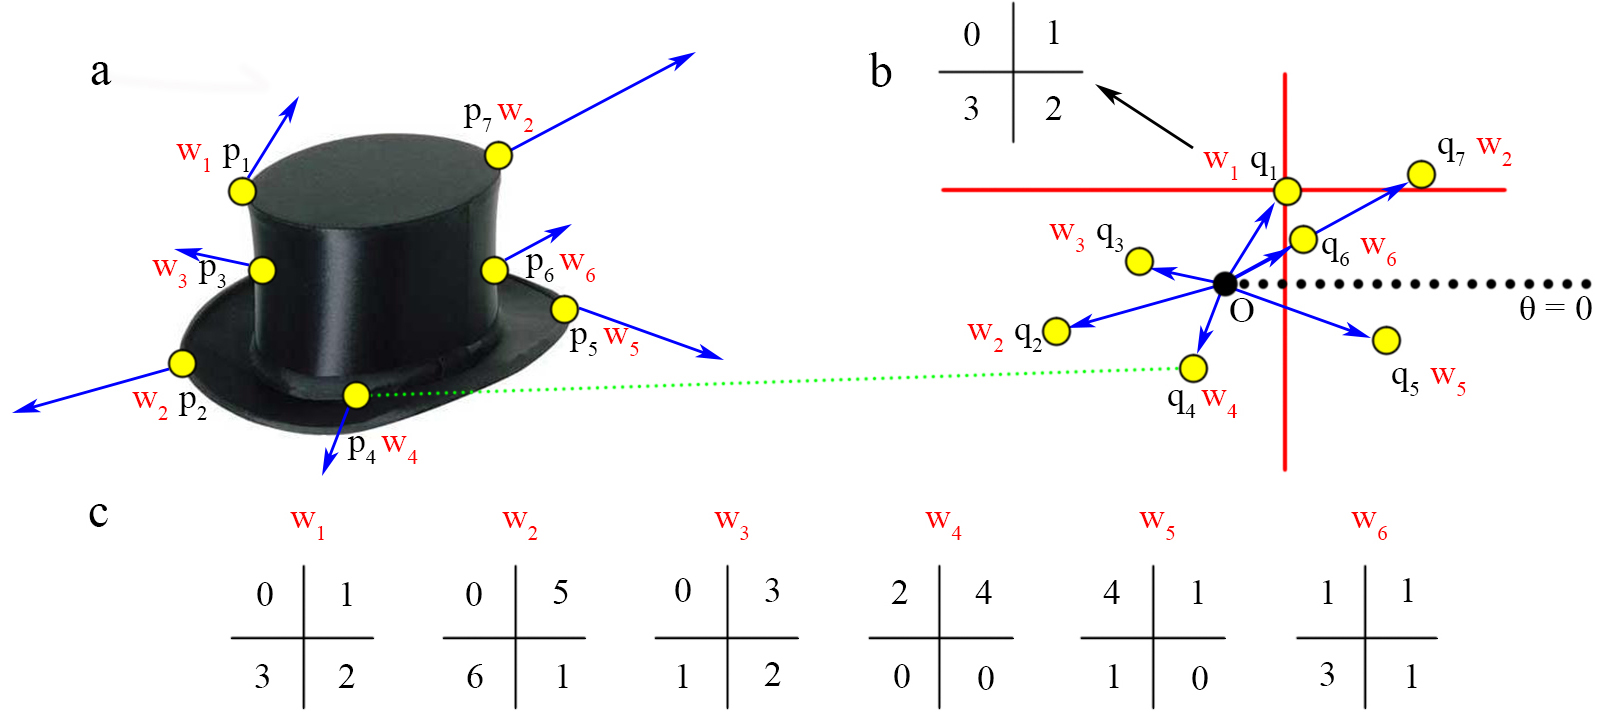
\includegraphics[width=\textwidth]{RSA.jpg}
	\caption{构建RPS和计算RSA向量实例}\label{fig:RSA}
\end{figure}
在一副图像$I$中,特征区域的集合可以表示为$R_I=\{r_I^{(1)},...,r_I^{(n)}\}$,其中$r_I^{(k)}$为第$k$个特征区域,$n$为特征区域的个数。如果只考虑特征区域的位置信息,例如\cite{lazebnik2006beyond}\cite{Cao2010Spatial}\cite{penatti2014visual}中的算法,则$R_I$将被简化为在图像直角坐标系$D$内的一个点集:
\begin{equation}
P_I=\{p_I^{(1)},...,p_I^{(n)}\}, ~~p_I^{(k)}=(x_I^{(k)},x_I^{(k)})
\end{equation}
其中,$x_I^{(k)}$和$x_I^{(k)}$表示特征区域$r_I^{(k)}$的横纵坐标。我们将这个空间定义为Region Position Space,表示为$S_{position}$。与编码$S_{position}$的信息相反,RSA试图编码特征区域的属性,即angle和scale。对于每个特征区域$r_I^{(k)} \in R_I$,它的scale和angle可以认为是在极坐标系$G$中的极径和极角,该极坐标系的极点为$O : \rho = 0$,极轴为$L : \theta = 0$。通过这种简化,我们将特征区域集合$R_I$转化为一个新的点集:
\begin{equation}
Q_I=\{q_I^{(1)},...,q_I^{(n)}\}, ~~q_I^{(k)}=(\rho_I^{(k)},\theta_I^{(k)})
\end{equation}
其中,$\rho_I^{(k)}$和$\theta_I^{(k)}$表示特征区域$r_I^{(k)}$的angle和scale。我们将这个空间定义为Region Property Space,表示为$S_{Property}$。

图\ref{fig:RSA}展示了创建$S_{Property}$的过程,其中(a)为$S_{position}$,(b)为$S_{Property}$,(c)为没有进行L1归一化的RSA向量,蓝色箭头标注了角度和尺度信息。$S_{position}$中的点与$S_{Property}$中的点具有一一对应关系,图\ref{fig:RSA}中的$p_4$和$q_4$描述了这种对应关系。通过建立$S_{Property}$,特征区域的属性的分布相当于$S_{Property}$中点的分布,并且通过这种变换,我们可以更加直接的编码属性的分布信息。图\ref{fig:RSA_dis}展示了一副典型自然图片的$S_{Property}$中的点的分布情况。
\begin{figure}[h]
	\centering
	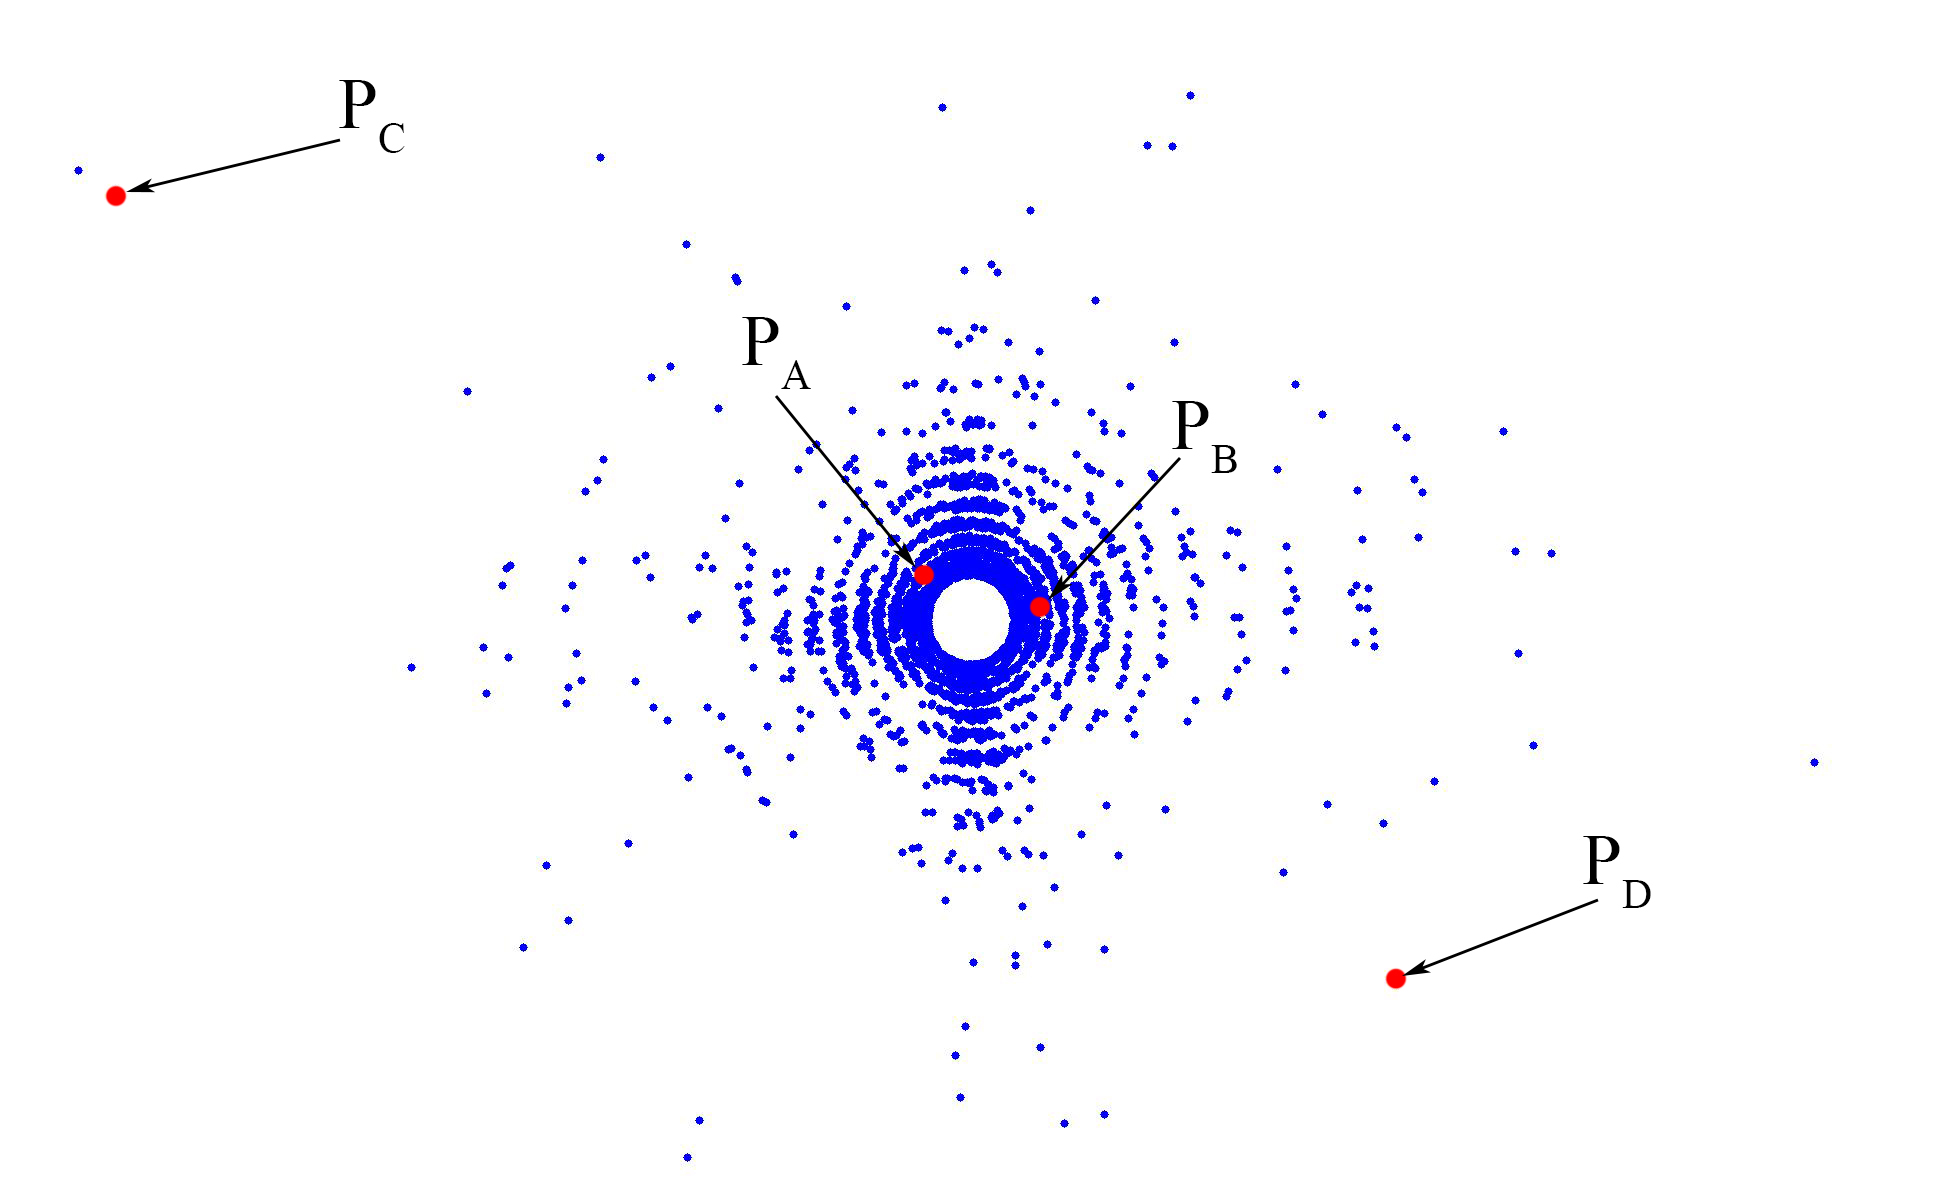
\includegraphics[width=\textwidth]{RSA_distribution.jpg}
	\caption{一幅典型自然图片的$S_{Property}$中的点的分布情况}\label{fig:RSA_dis}
\end{figure}

\subsection{RPS中点的分布}
\begin{figure}[h]
	\centering
	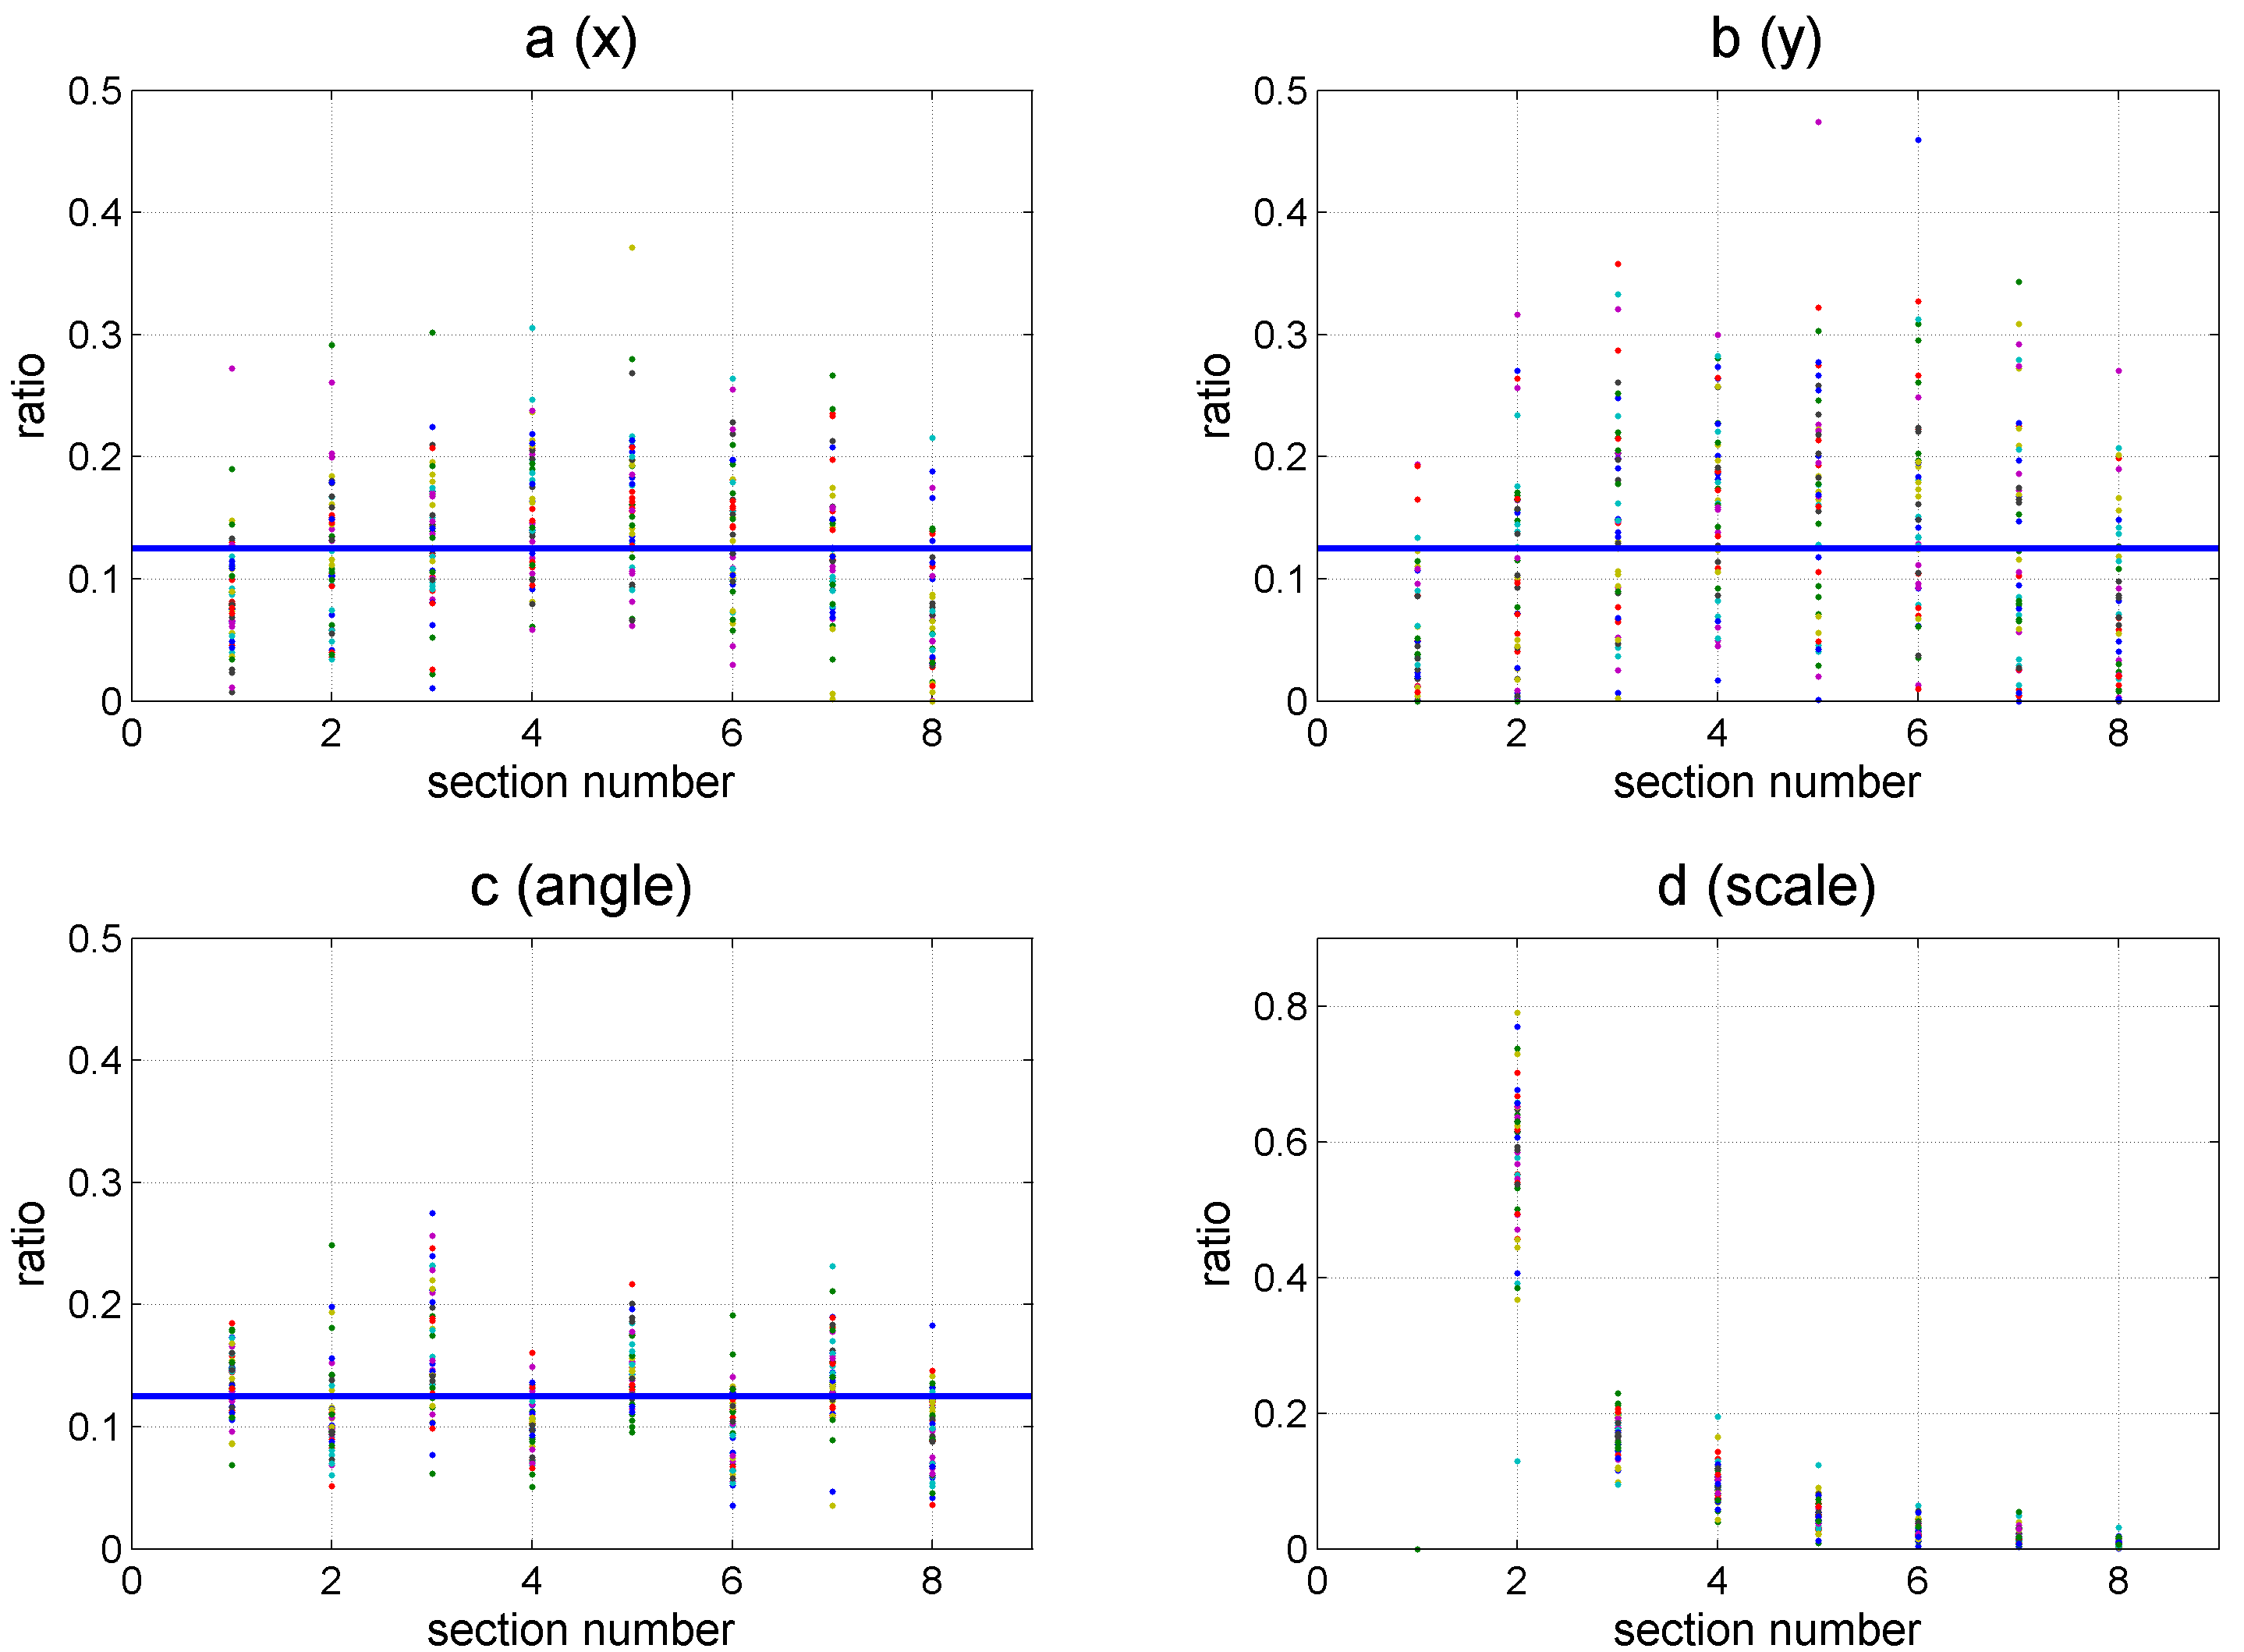
\includegraphics[width=\textwidth]{RSA_distribution_2.png}
	\caption{$S_{position}$和$S_{Property}$中的点的分布情况对比}\label{fig:RSA_dis_2}
\end{figure}
虽然在$S_{Property}$和$S_{position}$中的点存在一一映射的关系,但是他们的分布却十分不同。图\ref{fig:RSA_dis_2}展示了从Oxford\cite{philbin2007object}数据库中随机抽取的50张图片共140,000特征区域在不同空间上的分布情况。我们分别按横纵坐标将$S_{position}$分成8个区域,并统计每个区域中点的个数,如图\ref{fig:RSA_dis_2}中的(a),(b)所示。我们同样将和$S_{Property}$划分成8个区域,划分方法为:都以极点为中心,将$S_{Property}$分成8个等面积的扇形(用来测试angle的分布,如图(c))和8个等面积的同心环(用来测试scale的分布,如图(d))。图\ref{fig:RSA_dis_2}(a)、(b)、(c)中的横线为均值。通过图\ref{fig:RSA_dis_2}可以看出,在$S_{position}$中点的分布接近随机,有较大的方差,而在$S_{Property}$中angle的分布却更接近于均匀分布。在$S_{Property}$中特征区域尺度的分布更加具有规律性,我们用一个二次函数用来进行模拟:
\begin{equation}\label{eq:scale}
n=
\begin{cases}
0 & \text{$0 \le s \le s_0$} \\
\frac{1}{\alpha s^2} & \text{$s \ge s_0$}
\end{cases}
\end{equation}
其中$n$表示特征区域的个数,$s$表示特征区域的尺度值,$s_0$是cut-off尺度值,表示几乎没有特征区域的尺度会小于$s_0$,$\alpha$是一个常数。这两种截然不同的分布特性由SIFT\cite{lowe2004distinctive}描述符的提取过程确定。SIFT通过DOG\cite{lowe2004distinctive}提取图标中的blob特征,一张图片中的blob完全依赖于图片的内容。因为自然图片中的内容是随机的,所以$S_{position}$中点的分布也是随机的。但是,自然图像更加趋向于包含小的blob(一大块像素相近的区域在自然图片中并不常见,即使是像天空这样的图像,这样的区域也只有少数几个。),并且这些blob的梯度方向在360度上是均匀分布的,这就导致了图\ref{fig:RSA_dis_2}中的特殊分布规律。对于一个分布具有很强规律的点集,我们可以用相同的结构包含更多的信息。并且,我们在$S_{Property}$点的分布规律基础之上提出了计算RSA向量的快速算法和Spatial Weighting,前者提高了检索速度,后者显著提高了检索的准确度。

\section{RSA向量}
构建RSA向量的方法与构建WSA\cite{penatti2014visual}向量的算法相似,其过程如下:
\begin{enumerate}
	\item 取$S_{Property}$中的某点作为原点,将$S_{Property}$分成四个象限(水平垂直分割);
	\item 统计四个象限内特征点的数目;
	\item 将这四个值进行L1归一化作为原点特征区域的RSA向量;
	\item 重复上述步骤,求出图片中所有特征点的RSA向量。
\end{enumerate}

通过上述步骤,对于每个特征区域我们会得到一个4维的L1归一化的RSA向量。如果特征区域量化为视觉单词,那么对应的每个视觉单词就伴随一个4维的RSA向量。假设字典长度为$v$,传统BoW检索框架会对每张图片生成一个$v$维的BoW向量。当使用RSA向量时,对于每张图片我们会构建一个$4 \times v$的RSA-BoW向量。RSA-BoW向量编码了视觉单词的尺度和角度的分布信息。图\ref{fig:RSA}(b)描述了构建RSA向量的过程。需要注意的是,当两个特征区域被量化到同一个视觉单词$w_j$时(例如图\ref{fig:RSA}中的$q_2$和$q_7$),我们将他们的RSA向量相加然后进行L1归一化作为$w_j$的RSA向量,这样我们就完全抛弃了传统BoW检索框架中的词频信息。例如,在量化之前,$w_1$的RSA向量为[1, 0, 3, 2],$w_2$的RSA向量为[5, 0, 6, 1]。 同一个视觉单词的RSA向量与WSA向量\cite{penatti2014visual}没有任何数值上的关系。

\subsection{旋转的RSA向量}
只需要对上述构建RSA向量的操作稍作改进就可以使RSA达到旋转不变性。在得到RSA向量之后,我们根据特征区域的主方向(angle)重新排列RSA向量中的四个值。具体来讲,我们将RSA向量的第一维固定为这个特征区域主方向所在象限的值,其余三个值逆时针进行旋转。如\ref{fig:RSA}中的$w_2$,其主方向在第三象限,则$w_2$旋转的RSA向量为[6, 1, 5, 0]。

\section{RSA的高区分性}
\begin{figure}[h]
	\centering
	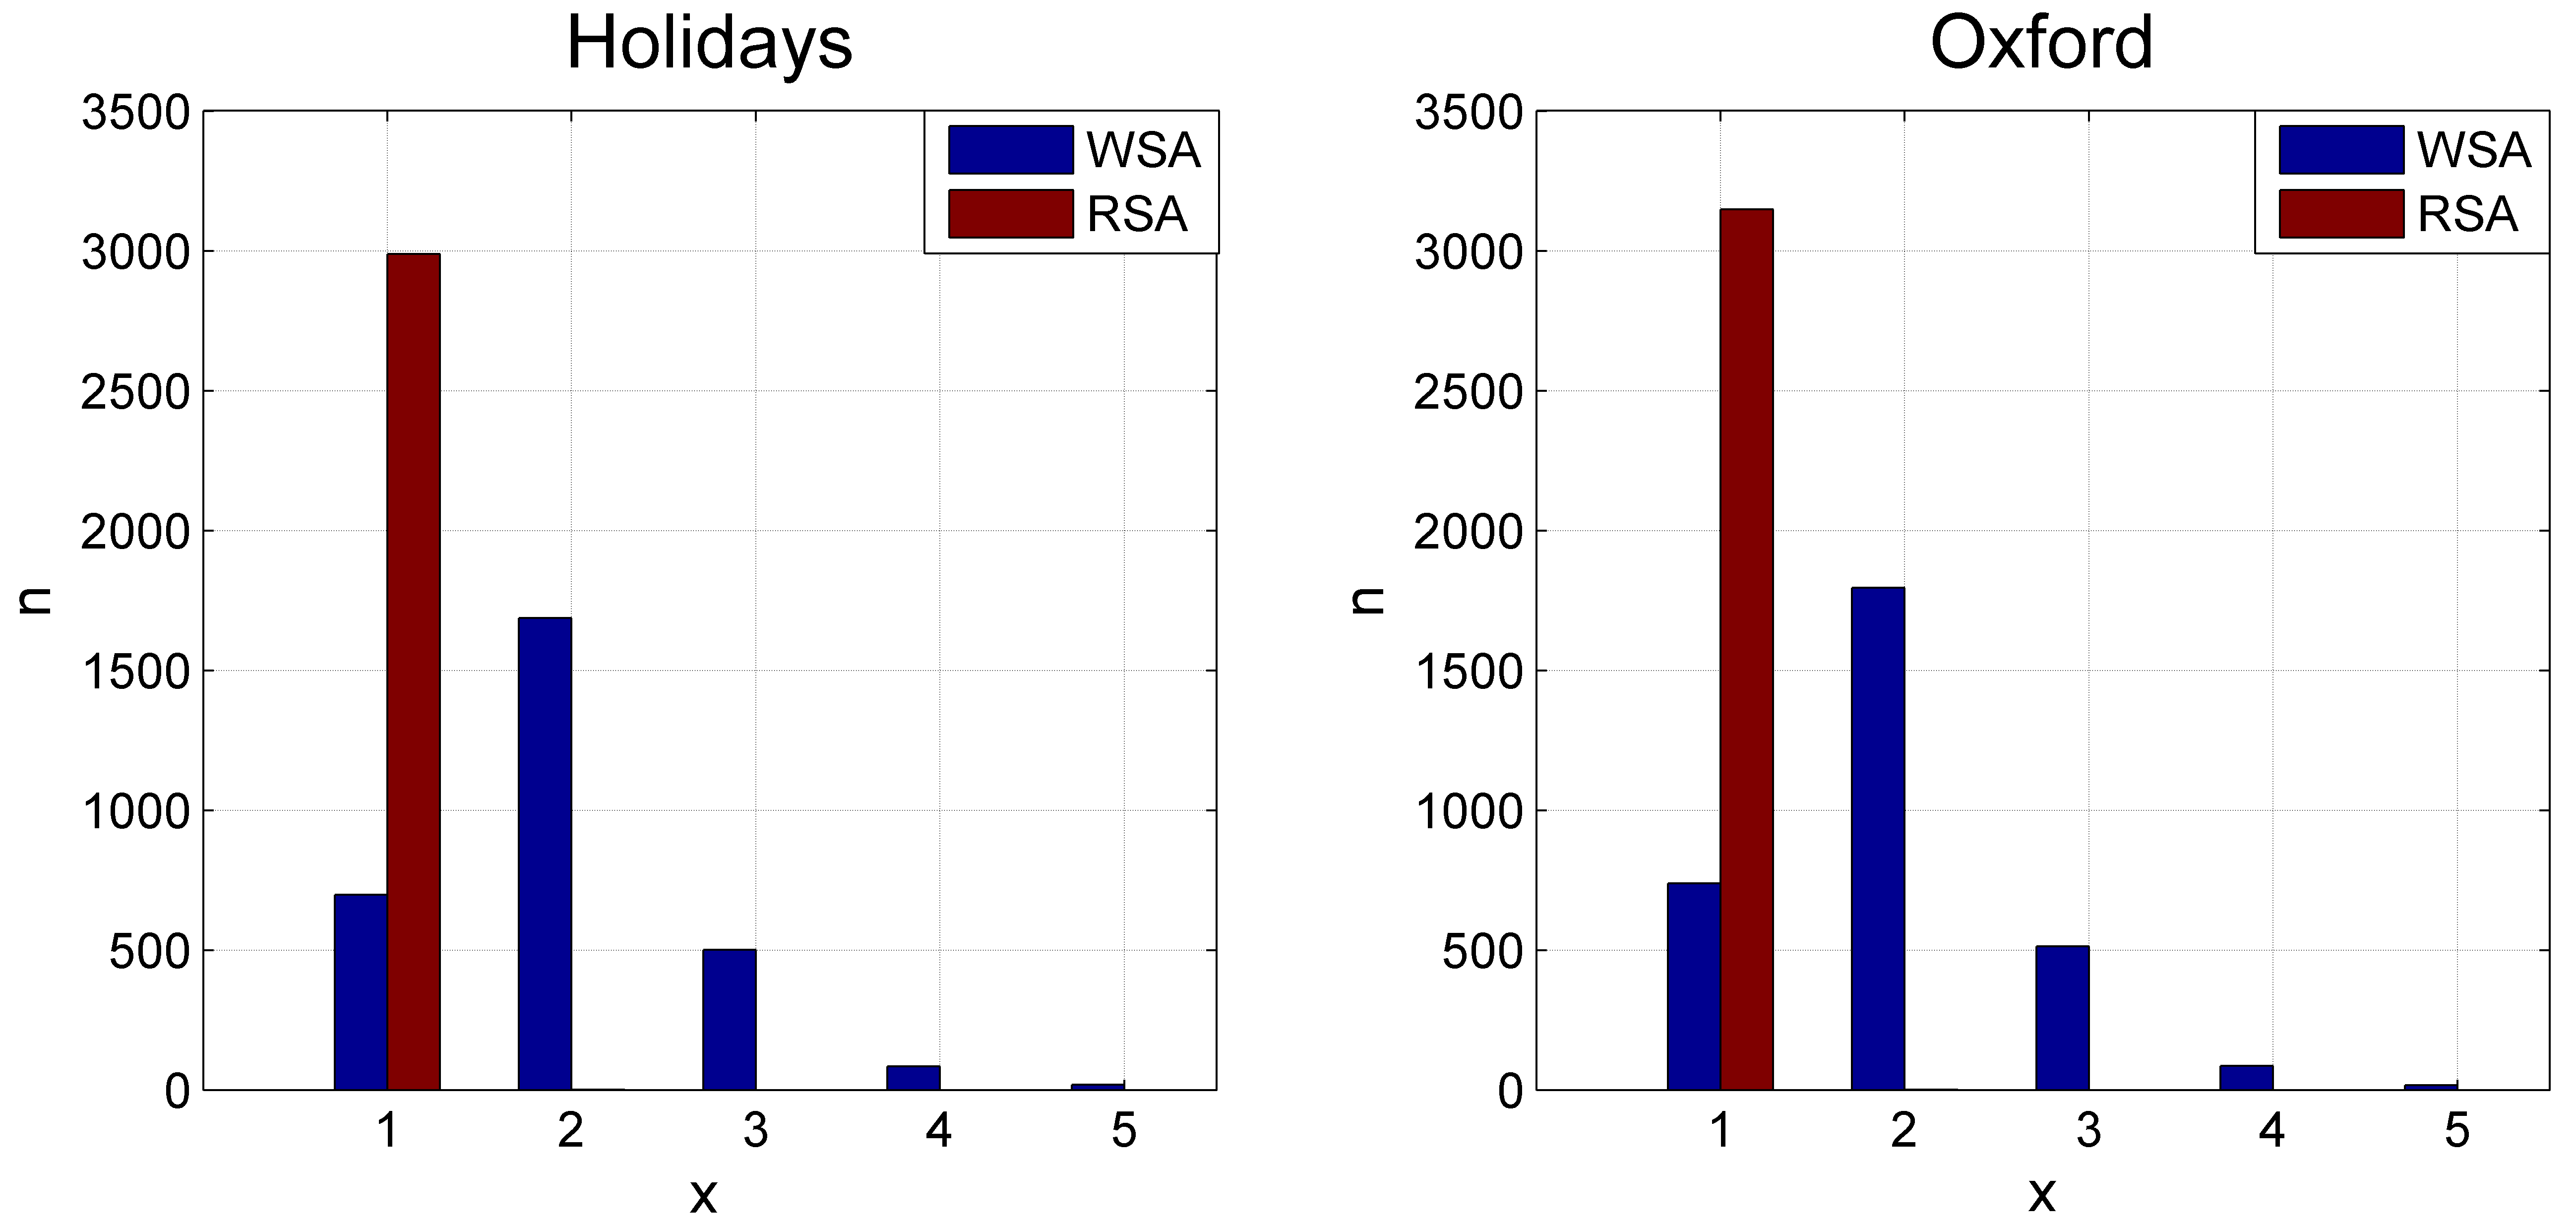
\includegraphics[width=\textwidth]{RSA_discrimination.png}
	\caption{WSA向量和RSA向量区分能力对比}\label{fig:RSA_disc}
\end{figure}
由于WSA\cite{penatti2014visual}基于特征点在图片中位置信息,所以WSA向量的值完全依赖视觉单词的坐标。但是,在实际图像检索过程中,很多特征区域的坐标是相同的。这是由于在构建SIFT\cite{lowe2004distinctive}特征时,有时候一个特征区域有不止一个主方向。此时,在同一个区域上会生成多个SIFT描述符,而它们的坐标都是一样的。这就导致了WSA向量区分能力不高,无法进行较严格的几何校验。于此相反,即使空间坐标相同,它们的梯度方向一定是不一样的,而RSA就是关注特征区域的angle和scale属性,这保证了RSA具有更高的区分能力。\ref{fig:RSA_disc}描述了WSA向量和RSA向量区分能力的对比情况。图中统计了在Holidays\cite{jegou2008hamming}数据集合Oxford\cite{philbin2007object}数据集上WSA和RSA向量的分布情况。图中的直方图(蓝色代表WSA向量,红色代表RSA向量)表示在一张图片中出现$x$次的向量平均数,例如$x=2$的cell表示在图片中出现两次的向量平均有多少。通过图\ref{fig:RSA_disc}我们可以看出,在一张图片中有75\%以上的WSA向量是重复的,而几乎没有重复的RSA向量,这证明了RSA的高区分性。

虽然在将$S_{Property}$中几乎没有重复的点,但是他们的RSA向量可以非常接近。就像在\ref{fig:RSA_dis}中的$p_A$和$p_B$。但是我们发现,这样的点几乎都分布在$S_{Property}$的原点附近,在后面章节中,我们提出了Spatial Weighting就是解决在$S_{Property}$原点附近出现的burstiness\cite{jegou2009burstiness}问题。

\section{计算RSA向量的快速算法}
为了计算一张图片所有视觉单词的RSA向量,我们需要遍历所有特征点,并且对于每个特征点,需要考虑其余特征点在$S_{Property}$的位置。这就使得计算图片RSA向量的时间复杂度为$O(n^2)$,其中$n$为图片中特征区域的个数。我们设计了一个可以更加快速计算图片所有RSA向量的算法,其核心思想很简单:
\begin{enumerate}
	\item 将$S_{Property}$按照特定的模式分成若干个区域,并统计每个区域内点的个数;
	\item 在计算某个点的RSA向量时,只对在坐标轴上的区域中的点进行重新计算。
\end{enumerate}
上述计算过程中,第一步只需要O(n)的时间复杂度,而第二步可以大大减少重复计算。

在$S_{Property}$中点规律的分布是上述思想可以对所有数据库图片有效的前提。Algorithm \ref{alg:1}给出了该算法具体的流程。
\renewcommand{\algorithmicrequire}{\textbf{Input:}} 
\renewcommand{\algorithmicensure}{\textbf{Output:}}
\begin{algorithm}
	\caption{computing the RSA vectors of an image}
	\label{alg:1} 
	\begin{algorithmic}[1]
		\REQUIRE Points set in $S_{property}$, that is $Q_I=\{q_I^{(1)},...,q_I^{(n)}\}$.
		\ENSURE RSA vectors of these points $R_I$.
		\STATE Initialize $N List$, each $List$ correspondences to a region in $S_{property}$;
		\STATE $R_I = \{\}$
		\FORALL {$q_I^{(k)}$ in $Q_I$}
		\STATE $index=$ the region that $q_I^{(k)}$ belongs to.
		\STATE put $q_I^{(k)}$ into $List[index]$.
		\ENDFOR
		\FORALL {$q_I^{(k)}$ in $Q_I$}
		\FOR {$i=0$ to $N-1$}
		\IF {$List[i]$ on the axes}
		\STATE re-count the points in $List[i]$.
		\ENDIF
		\ENDFOR
		\STATE update $R_I[k]$
		\ENDFOR
	\end{algorithmic} 
\end{algorithm}

我们设计了三种模式来划分$S_{Property}$,如图\ref{fig:RSA_d}。这三种模式分布将分$S_{Property}$分成了8、16和25个区域,并且在划分时我们考虑了点在$S_{Property}$中的分布特性,尽量使每个区域中点的数目均衡。算上暴力算法(可以认为只将$S_{Property}$划分成一个区域的特殊情况),我们将这四种算法的结果列在表\ref{tab:divide}中。我们列出了计算Holidays数据集所有图片的RSA向量所需的时间和对应的理论加速比(theoretical SR)和实际加速比(actual SR),theoretical  SR和actual SR的定义如下:
\begin{equation}
theoretical-SR = \frac{\#\text{all regions}}{\#\text{regions on axes}}
\end{equation}
\begin{equation}
actual-SR = \frac{time(\text{brute\_force})}{time(\text{divide\_x})}
\end{equation}
其中$\#$表示计数,$time()$表示所需时间。通过表\ref{tab:divide}我们可以看出,如果$S_{Property}$的分割模式与$S_{Property}$中点的分布契合,实际的加速比将逼近于理论加速比。由于在$S_{position}$中点的分布不具有$S_{Property}$中的规律性,无法得到最优的划分模式,所以这里提出的加速算法只适用于RSA向量的计算。

\begin{figure}[h]
	\centering
	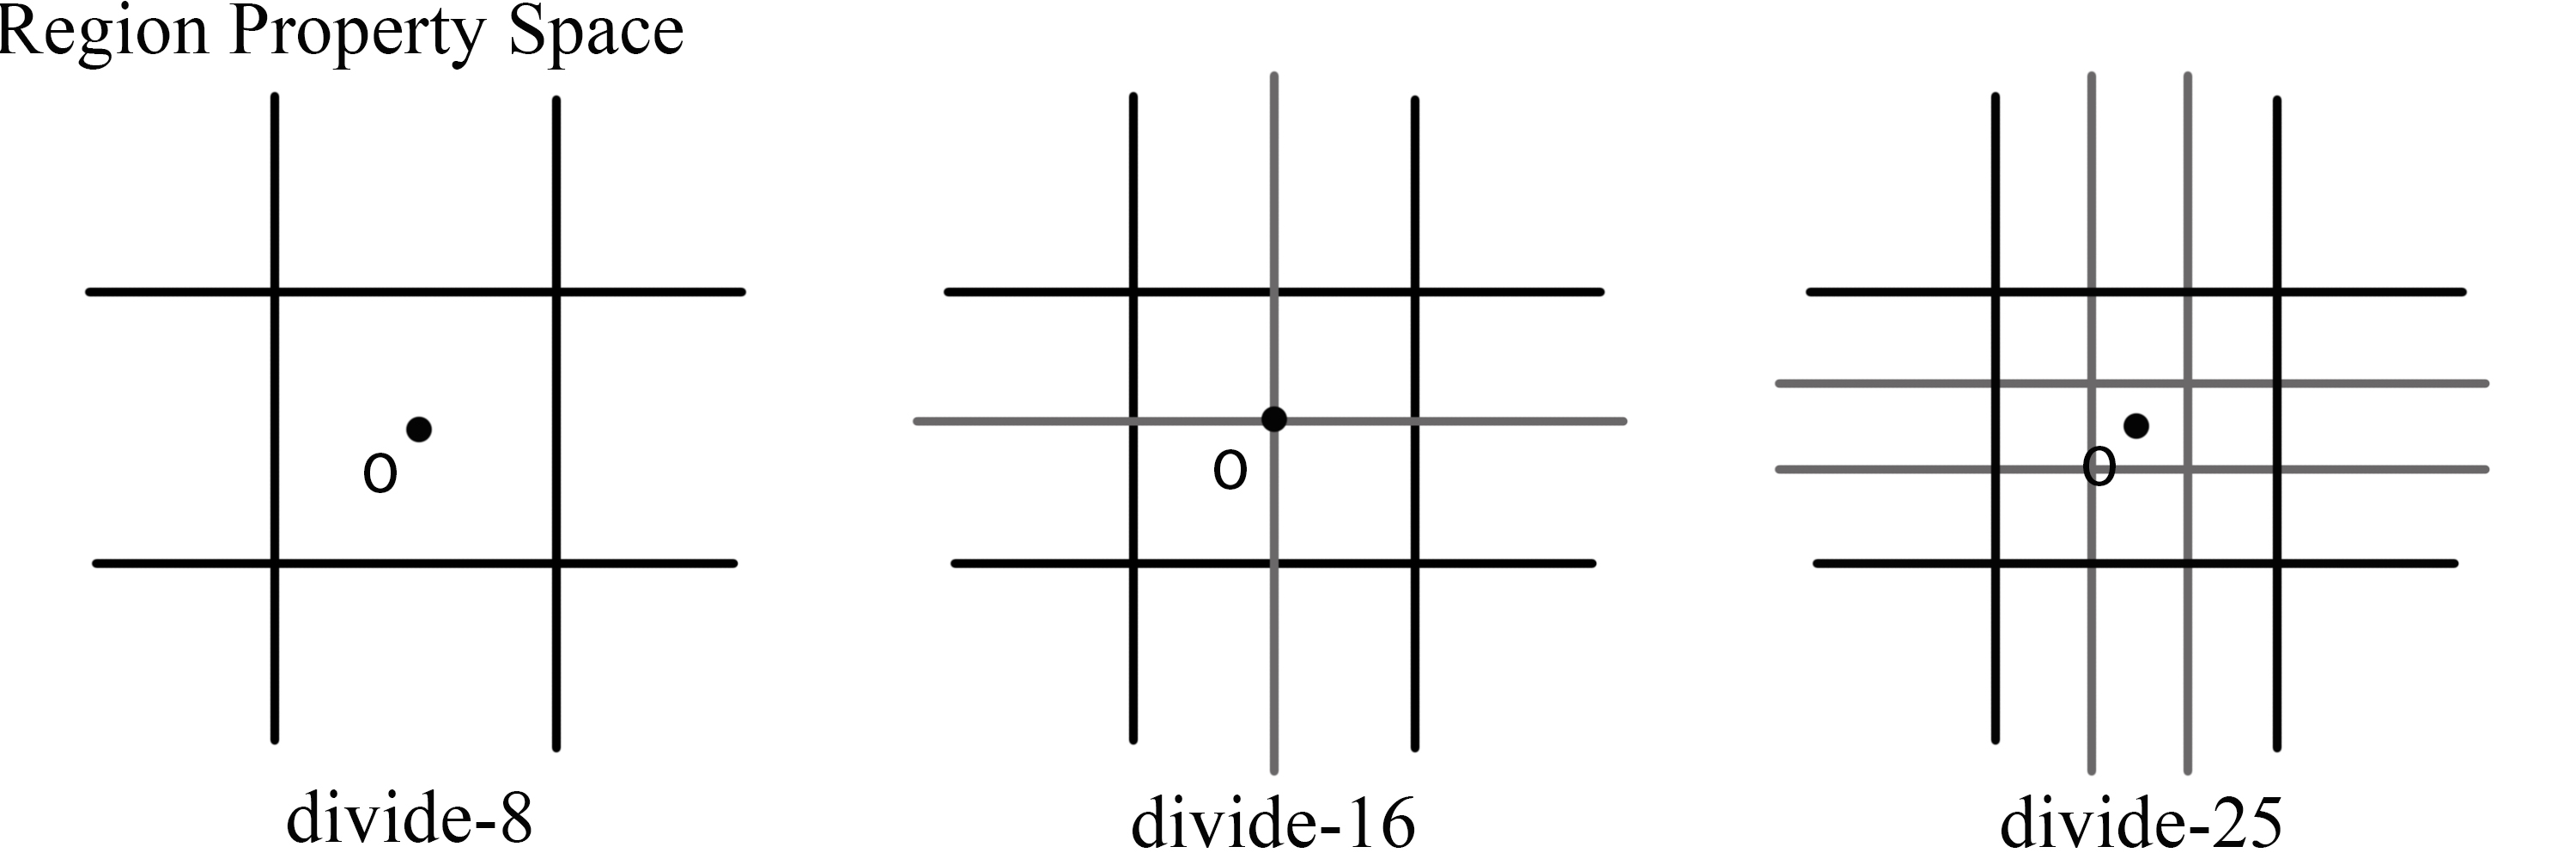
\includegraphics[width=\textwidth]{RSA_divide.jpg}
	\caption{划分$S_{Property}$的三种模式}\label{fig:RSA_d}
\end{figure}

\begin{table}
	\begin{center}
		\begin{tabular}{|l|c|c|c|c|}
			\hline
			& brute-force & divide-8  & divide-16 & divide-25 \\
			\hline
			time(s)    		& 461.4       & 281.8     & 200.7     & 187.7 \\
			theoretical SR	& 1.00        & 1.80      & 2.29      & 2.8 \\
			actual SR		& 1.00        & 1.64      & 2.28      & 2.45 \\    
			\hline
		\end{tabular}
	\end{center}
	\caption{使用不同算法计算RSA向量的时间复杂度对比}
	\label{tab:divide}
\end{table}

\section{Spatial Weighting}
\subsection{相似度计算}
在使用RSA进行图像检索时,通过公式\ref{eq:sim1}来计算图像之间的相似度。
\begin{equation}\label{eq:sim1}
S_{QI} = \frac{\sum_{j=1}^vsum(RSA_j^Q \cap RSA_j^I)}{N_Q + N_I}
\end{equation}

其中,$S_{QI}$表示查询图片$Q$和数据库图片$I$之间的相似性,$v$是视觉字典的长度;$(RSA_j^Q \cap RSA_j^I)$表示$Q$和$I$的第$i$个RSA向量的直方图相交的结果;$sum$表示向量中每一维的总和;$N_Q$和$N_I$表示图片$Q$和$I$包含的特征数。

\subsection{Burstiness}
\begin{figure}[h]
	\centering
	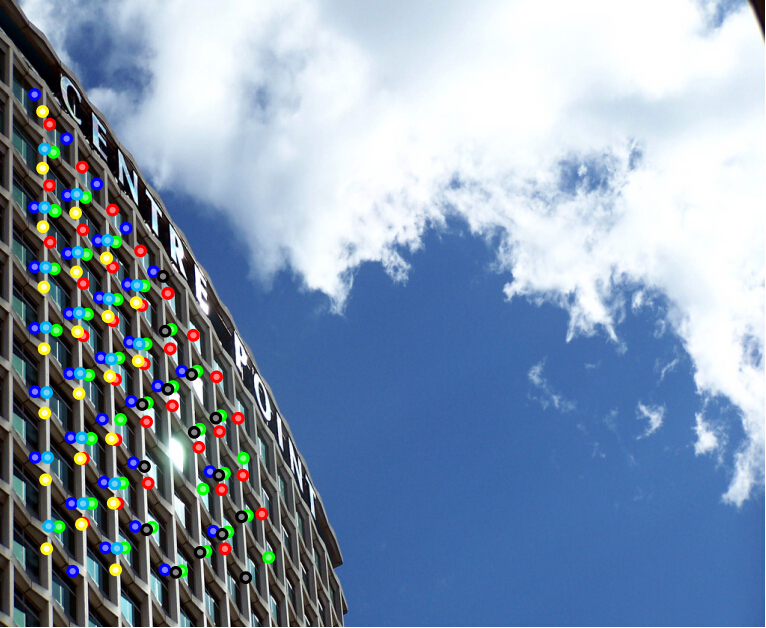
\includegraphics[width=0.8\textwidth]{burstiness.jpg}
	\caption{图像检索中的burstiness现象}\label{fig:burst}
\end{figure}

由于图片中大量存在重复的结构,如自然图片中的草地的纹理、建筑物图片中的窗户等,因此burstiness\cite{jegou2009burstiness}在图片检索中是一种常见的现象。burstiness现象最初发现于文本检索中。人们发现当某篇文档中出现了某个特定的单词,那么这个单词极有可能在该文档中还会出现。在基于BoW的图像检索框架中同样存在burstiness现象,图\ref{fig:burst}就描绘除了一张建筑物图片中存在的burstiness现象。burstiness现象会严重影响图像检索的精度,因为它过分增加了某些特征的重要性。在传统的TF-IDF加权模型中,由于burstiness现象,某些视觉单词的TF值会非常大,导致检索时的误匹配。例如,在检索过程中,如果一张数据库图片包含了图\ref{fig:burst}中的burstiness视觉单词,则该视觉单词会与所有图\ref{fig:burst}中的这些视觉单词匹配,导致严重的误匹配。

人们对图像检索中的burstiness现象同样进行了广泛的研究:\cite{Zhong2015Fast}提出了使用$1+\log (tf)$替换TF-IDF中的$tf$项来降低词频过高的影响;\cite{jegou2008hamming}深入研究了intra-image和inter-image的burstiness现象,并且提出相应的解决方案,在检索时减少误匹配的发生;\cite{shi2015early}通过统计学的方法,在进行检索前发现并去除burstiness的视觉单词。

\subsection{改进的相似度计算}
在基于RSA几何校验的图像检索方案中,同样存在burstiness的问题。如图\ref{fig:RSA_dis}中所示,接近$S_{Property}$极点的视觉单词将具有相似的RSA向量,这同样会导致在检索时产生误匹配。基于$S_{Property}$中点特殊的分布模式,对此我们提出了一种新的加权方案Spatial Weighting(SpW)。相比于TF-IDF加权模型,SpW是一种局部的加权方案,这是由于计算SpW时,只考虑对应两个视觉单词在$S_{Property}$中的位置关系。通过公式\ref{eq:scale}我们可以看出一个特征区域更加趋向于有较小的scale,因而它在$S_{Property}$中更可能位于极点附近,我们将这种特征区域标记为$q_s$。于此相反,我们将那些具有较大尺度,远离极点的特征区域标记为$q_l$。$q_s$和$q_l$具有以下特点:
\begin{enumerate}
	\item 在一张图片中$q_s$出现的概率高,并且$q_s$所对应的RSA向量的四个值的方差较小;
	\item 在一张图片中$q_l$出现的概率低,并且$q_l$所对应的RSA向量的四个值的方差较大,一般具有一个或两个峰值;
	\item 在检索时$q_s$容易发生误匹配,而$q_l$不容易发生误匹配。
\end{enumerate}

SpW的思想就是减小$q_s$的权重,增加$q_l$的权重,所以改进的相似度计算公式如下:
\begin{equation} \label{eq:sim2}
S_{QI} = \frac{\sum_{j=1}^vspw_j \times sum(RSA_j^Q \cap RSA_j^I)}{N_Q + N_I}
\end{equation}
其中,
\begin{equation} \label{eq:sim3}
spw_j = (\max(RSA_j^Q \cap RSA_j^I))^r
\end{equation}

其中,$r$控制了SpW权重施加的力度。实验表明,当$r=2$时可以达到最优的检索精度,这也符合公式\ref{eq:scale}。SpW具有以下优点:
\begin{enumerate}
	\item 计算复杂度低,几乎不增加检索时间;
	\item 可以一定程度上减弱burstiness现象对检索性能的影响;
	\item 可以保证正确的匹配具有较大的权重。
\end{enumerate}

\section{大规模图像检索框架}
在进行大规模的图像检索,尤其是图片数据规模在百万以上时,要求检索引擎有较快的相应时间和低内存占用。为此,我们提出了量化的RSA向量,并将RSA向量直接编码到倒排表中,保证了检索的性能。

\subsection{量化的RSA向量}
如果直接的表示一个RSA向量,则我们需要4个浮点数,这是传统的BoW模型的四倍($tf\_idf$值只需要一个浮点数表示)。为了可以节省空间,我们将RSA向量进行量化,每个RSA浮点数被量化到一个无符号的字符类型(8 比特),这样表示一个RSA向量只需要32比特,相当于一个浮点数,与传统的BoW模型占用相同的内存。表\ref{tab:quantization}列出了在三个数据集上量化对RSA效果的影响,其中“Original”表示没有进行量化,“Quantized”表示进行了量化。通过表\ref{tab:quantization}我们发现,量化操作并没有明显的影响RSA的性能,这可能是由于RSA原本就是编码图片的全局信息,抗噪声能力强,量化的RSA保持了它的高区分能力。这同时也证明了RSA适合大规模检索的应用。在实验部分,所有RSA向量都是经过量化的。
\begin{table}
	\begin{center}
		\begin{tabular}{|c|c|c|c|}
			\hline
			& Holidays       & Oxford5K         & Paris\\
			& 20K~~~~~ 200K  & 500K~~~~ 1M    & 500K~~~~ 1M\\
			\hline\hline
			Original    & 0.631 ~ 0.691  & 0.754 ~ 0.803  & 0.781 ~ 0.795\\
			Quantized	& 0.627 ~ 0.690  & 0.760 ~ 0.809  & 0.772 ~ 0.796\\
			\hline
		\end{tabular}
	\end{center}
	\caption{量化与非量化的RSA性能对比} 
	\label{tab:quantization}
\end{table}

\subsection{倒排索引结构}
在进行大规模图像检索时,我们同样使用经典的倒排索引结构。图\ref{fig:ii}显示了我们的倒排索引结构:每个视觉单词指向了一个包含该视觉单词的列表;在该列表中,除了包含必须的图片ID外,还包含了该视觉单词在该图片中的RSA向量值。通过量化操作,该倒排表与传统的BoW模型中的倒排表占用相同的内存。图像检索过程相当于累加RSA向量相似度得分的过程,一张图片的最终得分为加权的RSA向量相似度得分和。
\begin{figure}[h]
	\centering
	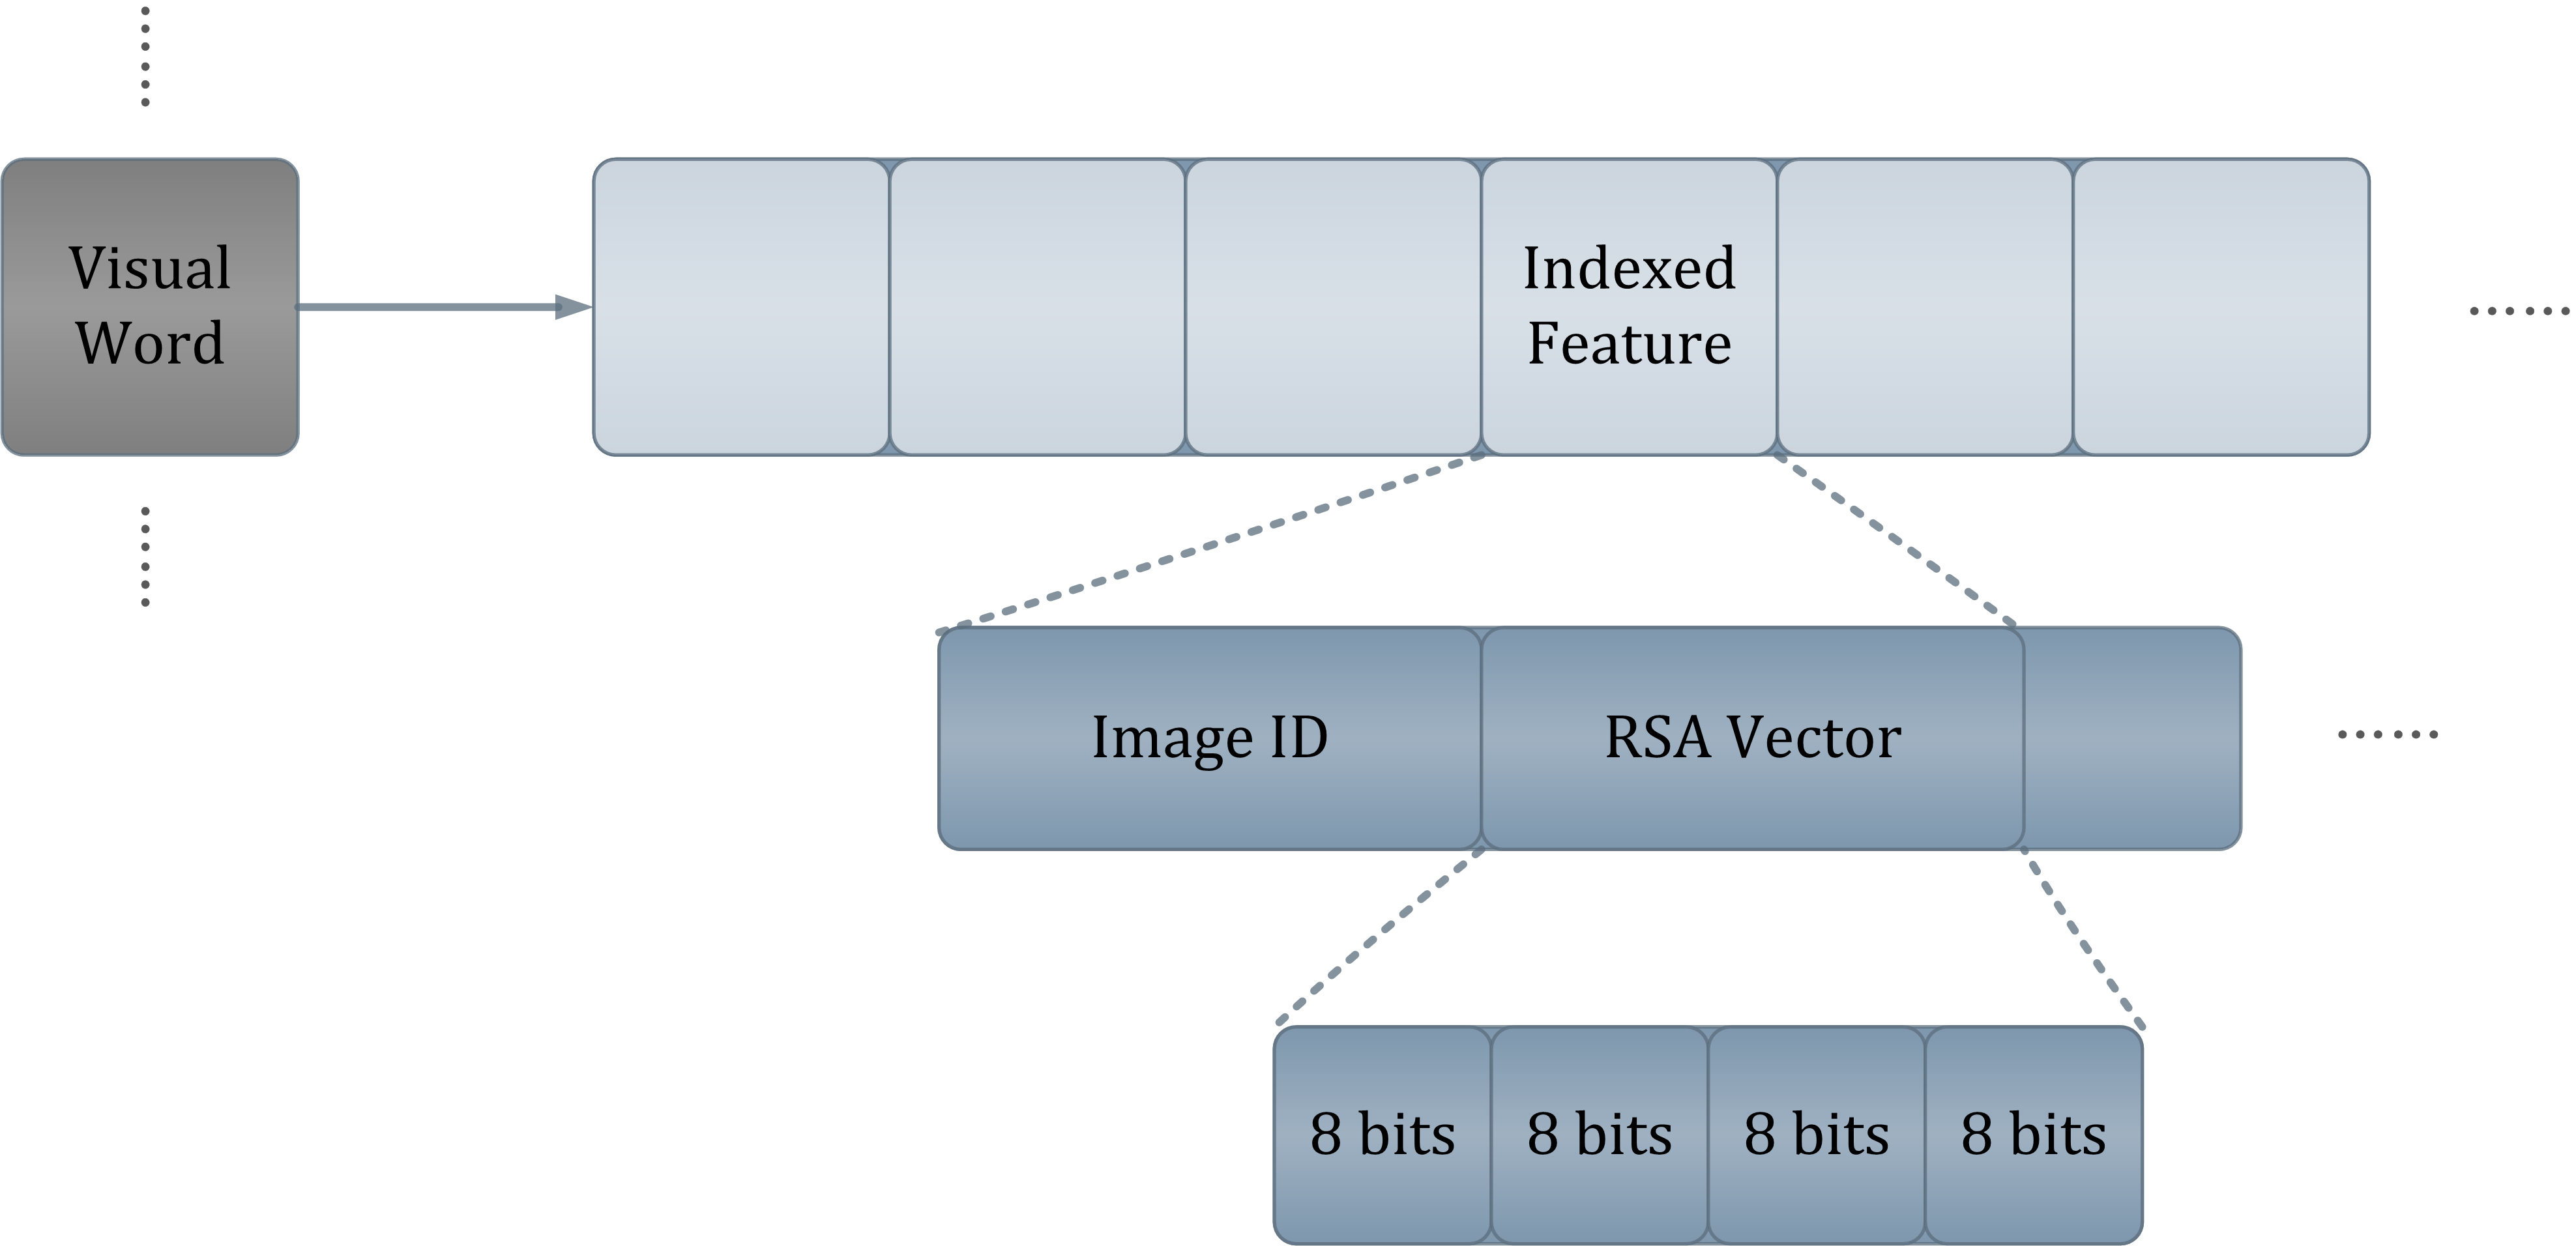
\includegraphics[width=0.8\textwidth]{Inverted_Index.png}
	\caption{包含RSA的倒排索引结构}\label{fig:ii}
\end{figure}


\section{实验}
我们的实验主要在Holidays\cite{jegou2008hamming}、Oxford5K\cite{philbin2007object}和Paris\cite{philbin2008lost}三个标准数据集上进行。这三个数据集可以测试多种变换和检索精度。在具体实验过程中,我们首先检测图片中的Hessian-Affine区域\cite{mikolajczyk2004scale},并在该区域上提取SIFT局部特征\cite{lowe2004distinctive}。为了应对实际图像检索中可能出现的旋转问题,我们并没有应用重力向量假设\cite{perd2009efficient}。为了快速构建视觉词典,我们使用了AKM\cite{philbin2007object}聚类算法。为了提高baseline,我们使用了改进的SIFT特征RootSIFT\cite{arandjelovic2012three}。为了可以与其他算法进行比较,我们使用标准的实验的参数:对于Holidays数据集,我们在一个独立的数据集上建立200K的视觉词典;对于Oxford5K和Paris我们构建了1M的视觉字典,并且考虑查询图片的输入区域。为了验证RSA算法在大规模数据库上的性能,我们测试了在Holidays+Flickr1M\cite{philbin2007object}上图像检索的性能。由于Holidays、Oxford5K和Paris无法测试尺度变换,我们在Copydays\cite{douze2009evaluation}上测试了RSA对尺度变化的鲁棒性。在Holidays数据集上,我们使用旋转的RSA向量,这是由于只有Holidays数据集中的图片可能有不同的方向。我们使用mAP(Mean Average  Pecision)度量检索的性能。

\subsection{数据集}

\subsubsection{Holidays}
Holidays数据集包含1,491张各种场景的图片。其中500张查询图片,并且大部分查询图片对应一到两张相似图片。该数据集可以测试图像检索中旋转、视角变换、模糊等情况。

\subsubsection{Oxford5K}
Oxford5K的5,062张图片包含了11个Oxford的地标性建筑。每个地标有5张查询图片,所以共有55张查询图片。每张数据库图片被分成以下等级:
\begin{enumerate}
	\item Good,相应的地标完整的显示在图片内;
	\item Ok,相应的地标至少有25\%的部分显示在图片内;
	\item Junk,无法确定其与地标的相关性;
	\item Absent,相应的地标不在图片内;
\end{enumerate}

根据一般规则,我们在计算mAP时不考虑标注为Junk的图片。

\subsubsection{Paris}
Paris数据集包含6,412张图片,这些图片通过在Flickr上搜索“paris landmarks”得到。Paris数据集同样包含55张查询图片,并且数据库图片具有与Oxford5K相似的标签。

\subsubsection{Copydays}
Copydays数据集包含了Holidays数据集中的157张图片。每张图片进行了人工处理,包括JPEG压缩、裁剪和其他变换。我们只使用经过JPEG压缩的部分数据。在这部分数据中,每张图片经过不同程度的压缩,包含9个等级,质量值范围为75至3。所以,我们共使用了1,570张图片。在这个数据集上我们使用topN检索图片的准确率(P@N)来度量检索性能。

\subsubsection{Flicker1M}
这个数据集包含从Flickr上下载的1,040,801张图片,主要用于测试算法的可扩展性。

\subsection{参数影响}
通过\ref{eq:sim2}和\ref{eq:sim3}我们可以发现,RSA的检索性能只由字典大小$v$和权重影响因子$r$来决定。这节将讨论这两个参数的影响并得到最优值。
\begin{figure}[h]
	\centering
	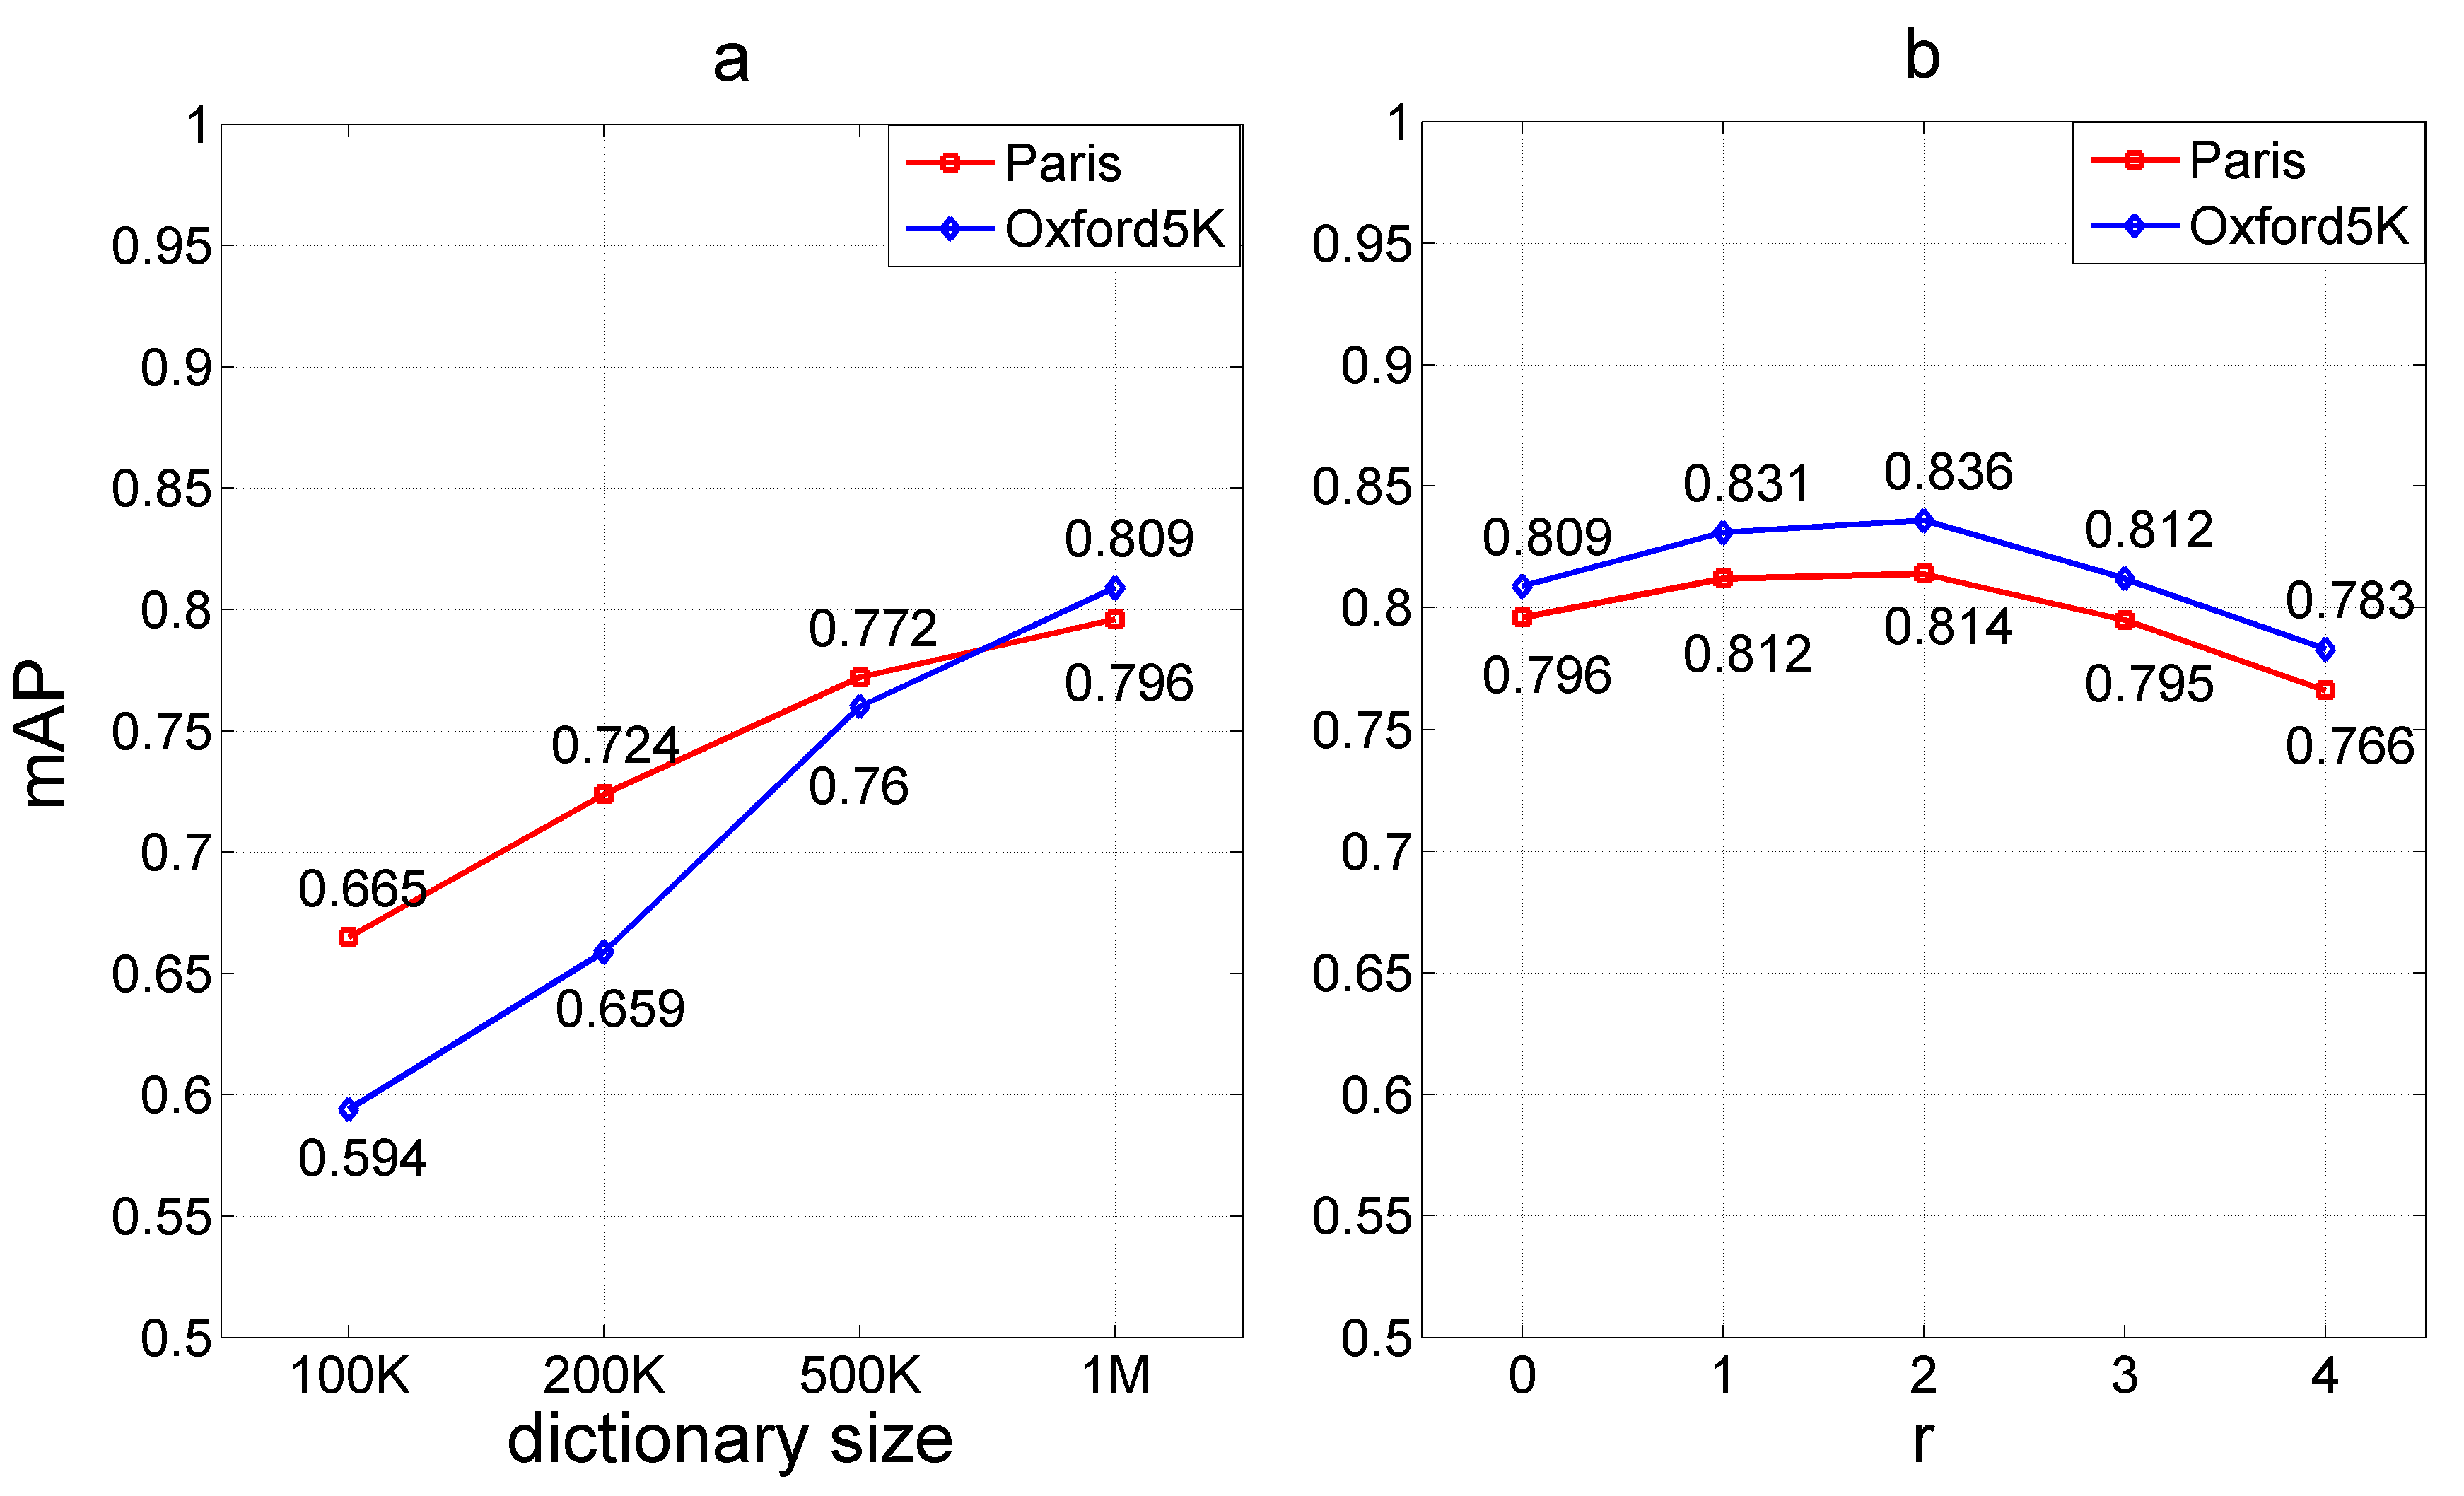
\includegraphics[width=0.8\textwidth]{dic_r.png}
	\caption{(a)字典大小对检索结果的影响;(b)权重影响因子$r$对检索效果的影响}\label{fig:dr}
\end{figure}

\subsubsection{字典大小$v$}
\ref{fig:dr}(a)给出了字典大小对检索结果的影响(没有使用SpW的情况),我们在Oxford 5K和Paris两个数据库上使用四种大小的字典进行了实验。通过实验结果可以看出,当字典变大时RSA会取得更好的检索mAP。其原因不仅是大字典可以增加视觉单词的区分能力,同时也提高的RSA向量的区分力。在计算RSA向量时,不同的特征区域可能会被量化到同一个视觉单词,这会导致其RSA的区分能力下降。较大的字典可以减少这种现象出现的概率。

\subsubsection{权重影响因子$r$}
SpW的目标是减弱在检索过中的burstiness现象,即在$S_{Property}$中,在极点附近出现点的概率要明显高于周围出现点的概率。参数$r$控制了SpW施加的力度,也就是对极点附件点权重的抑制程度,$r$越大,极点附近点的权重就越低。理论上,当$r$的取值符合公式\ref{eq:scale}中刻画的分布情况时,SpW达到最优的检索效果。图\ref{fig:dr}(b)展示了$r$不同取值下的mAP。通过该实验可以看出,当$r=2$时,SpW达到最优的性能,这也是符合我们的期望的。在后续的试验中,我们固定$r=2$。

\subsection{RSA和SpW的性能}
\begin{table}
	\begin{center}
		\begin{tabular}{|c|c|c|c|}
			\hline
			& Holidays       & Oxford5K         & Paris\\
			& 20K~~~~~ 200K  & 500K~~~~ 1M    & 500K~~~~ 1M\\
			\hline\hline
			baseline  & 0.566 ~ 0.611  & 0.651 ~ 0.685  & 0.674 ~ 0.681\\
			\hline
			~WSA      & 0.721 ~ 0.742  & 0.743 ~ 0.792  & 0.779 ~ 0.804\\
			*WSA      & 0.717 ~ 0.737  & 0.764 ~ 0.793  & 0.783 ~ 0.790\\
			\hline
			~RSA      & 0.757 ~ 0.775  & 0.760 ~ 0.809  & 0.772 ~ 0.796\\
			*RSA      & \textbf{0.800} ~ \textbf{0.806} & \textbf{0.802} ~ \textbf{0.836} & \textbf{0.803} ~ \textbf{0.814}\\
			\hline
		\end{tabular}
	\end{center}
	\caption{在Holidays、Oxford5K和Paris数据集上的检索结果}
	\label{tab:map1}
\end{table}

表\ref{tab:map1}比较了RSA与BoW baseline和WSA\cite{penatti2014visual}的检索性能,其中*表示使用SpW。为了使RSA方法达到较高的检索精度,在Holidays数据集的试验中,我们融合了HE\cite{jegou2008hamming}和HE Weighting\cite{jegou2009burstiness}方法。通过表\ref{tab:map1}可以看出,WSA和RSA对BoW baseline都有明显的提升,尤其是RSA算法。RSA算法在大多数情况下都比WSA得到更优的检索结果。因为RSA只编码了特征区域的属性信息,所以我们可以得出结论:特征区域的属性信息要比特征区域的位置信息\cite{penatti2014visual},和在图片中出现的频率信息具有更高的区分能力。

\subsubsection{SpW带来的提升}
SpW带来的效果提升是很明显的。在Holiday O型和Oxford5K数据集上,SpW可以将RSA的结果提升5\%;在Paris数据集上,SpW同样可以带来4\%的提升。SpW的设计针对$S_{Property}$点的特殊分布模式,所以SpW对WSA算法没有效果。

\subsubsection{与其他空间校验算法的比较}
\begin{table}
	\begin{center}
		\begin{tabular}{|c|c|c|c|c|c|c|}
			\hline
			Dataset   & RSA     & \cite{jegou2009burstiness}   &\cite{wang2011contextual}    & \cite{Zhong2015Fast}    & \cite{Zhong2015Fast}(gv)  &\cite{babenko2014neural}\\
			\hline\hline
			Oxford5K  & 0.836   & -      & -      & 0.746  & \textbf{0.850}  & 0.557\\
			\hline
			Paris     & \textbf{0.814}   & -      & -      & 0.725  & \textbf{0.814}  & -\\
			\hline
			Holidays  & 0.806   & \textbf{0.807}  & 0.780  & 0.720  & 0.771  & 0.789\\
			\hline
		\end{tabular}
	\end{center}
	\caption{RSA与state-of-the-art算法的比较}
	\label{tab:map2}
\end{table}

我们将RSA算法与目前比较优秀的几何校验算法进行了比较,包括WGC\cite{jegou2008hamming}\cite{jegou2009burstiness},SCW\cite{wang2011contextual},DSM\cite{Zhong2015Fast}和Neural Code\cite{babenko2014neural}。表\ref{tab:map2}列出了比较的结果,其中gv表示使用了重力向量假设。通过表\ref{tab:map2},我们发现RSA在Holidays数据集上得到了与\cite{jegou2009burstiness}相近的结果。但是由于RSA将空间信息编码到BoW向量中,在检索时完成校验,而WGC是一种后检验方法,所以RSA在检索效率上要高于WGC,这点可以通过表\ref{tab:time}得到验证。具有重力向量假设的DSM在Paris得到了与RSA相同的结果,并在Oxford5K上得到了高于RSA的结果。DSM得到的高mAP是因为它使用了更加严格的限制,但是在实际的图像检索的场景下,图片旋转是很常见的,此时无法保证重力向量假设。在同样使用普通的SIFT描述符\cite{lowe2004distinctive}时,RSA的检索结果要远远高于DSM。所以,相比于DSM,RSA更适合一般情况下的大规模图像检索。

\begin{table}
	\begin{center}
		\begin{tabular}{|c|c|c|c|c|}
			\hline
			Method         & RSA & baseline & \cite{jegou2009burstiness} & \cite{wang2011contextual}\\
			\hline
			Query Time (s) & 0.625 & 0.623 & 0.858 & 0.676\\
			\hline
		\end{tabular}
	\end{center}
	\caption{在Holidays+Flickr1M数据集上不同算法的查询时间(单核CPU)}
	\label{tab:time}
\end{table}

\subsubsection{大规模图像检索}
\begin{figure}[h]
	\centering
	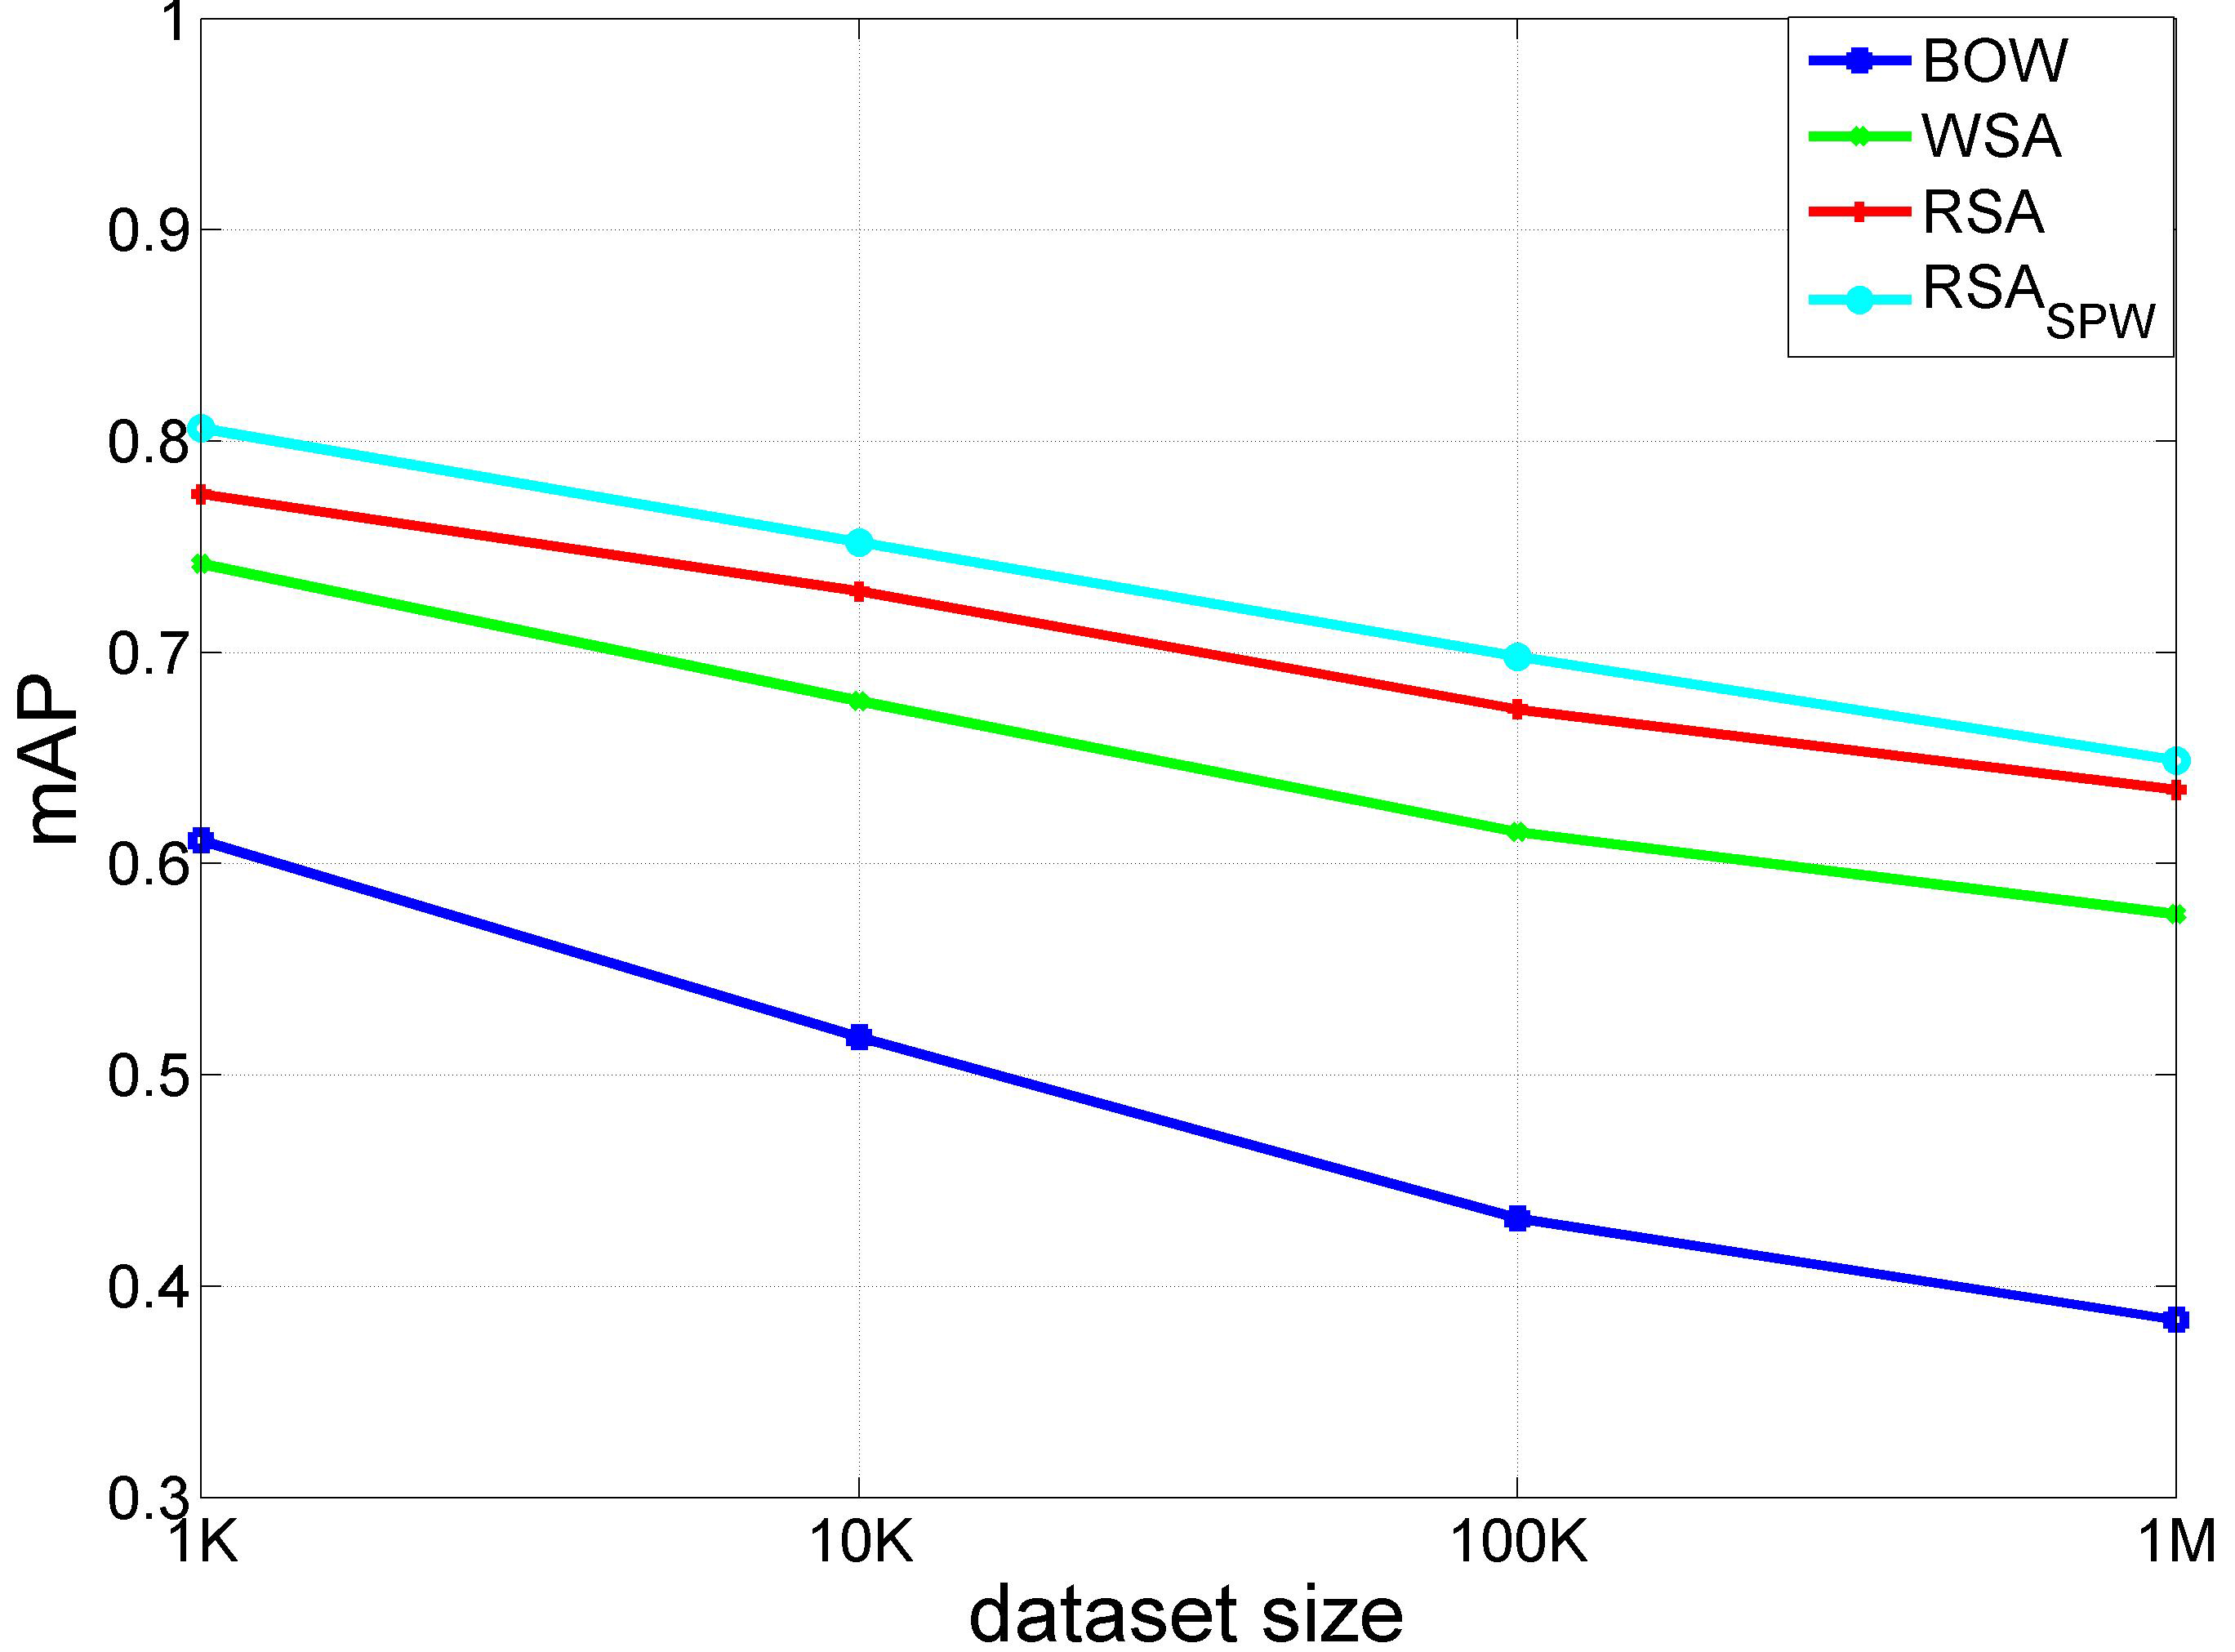
\includegraphics[width=0.6\textwidth]{large_scale.jpg}
	\caption{在Holidays+Flickr1M数据集上的检索结果}\label{fig:ls}
\end{figure}
为了验证RSA的可扩展性,我们在Holidays+Flickr1M数据集上进行了实验(数据集图片总量超过一百万)。图\ref{fig:ls}描绘了RSA、WSA和BoW baseline在大规模数据集下的检索性能,其中字典大小为200K。通过图\ref{fig:ls}我们可以看出在图像库达到百万级别时,RSA可以将mAP从0.384提高到0.694,并且RSA的检索结果要比WSA高13\%。另一方面,通过表\ref{tab:time},RSA几何校验算法所带来的时间增加几乎可以忽略不计。这些实验结果表明,RSA不仅可以显著提升BoW检索的准确率,同时不会带来额外的计算复杂度,是大规模图像检索场景下合适的解决方案。

\subsection{对尺度和角度变化的鲁棒性}
由于RSA算法建立在图像特征区域的属性上,一个明显的问题是RSA可不可以解决图片尺度变化和旋转的问题。angle和scale变化的问题是几何校验中的难点,至今没有很好的解决方案。WGC\cite{jegou2008hamming}为了应对上述问题,认为图片只有4个可能的角度并且图片的尺度是不会改变的,这严重限制了该算法的应用场景。由于RSA编码的是图片全局的几何信息,并且具有较强的鲁棒性,所以RSA可以很好的应对图片尺度变化和旋转的问题。

\subsubsection{图片的尺度变化}
由于图片尺度的变化不会影响点在$S_{Property}$中的相对位置关系,所以RSA不受图片尺度变化的影响。\ref{fig:rsa_s}展示了RSA在Copydays上的检索结果。其中,Copydays上的图片只包含尺度变化,我们使用P@N来度量检索结果,10代表最高准确率。通过图\ref{fig:rsa_s}我们发现,RSA与BoW具有相似的检索结果,这表明RSA不受图片尺度变化的影响,并且SpW同样可以显著提高检索性能。

\subsubsection{图片的旋转}
图片的旋转会改变点在$S_{Property}$的相对位置,但是我们提出的旋转的RSA向量可以很好的应对这个问题。图\ref{fig:rsa_r}展示了旋转的RSA在Holidays数据集上的部分检索结果。其中,绿框表示查询图片,每个查询图片都有旋转版本的相似图片,红框表示没有找到的相似图片。通过图\ref{fig:rsa_r},我们可以看出这些旋转的相似图片几乎可以被RSA算法正确检索。

\begin{figure}[h]
	\centering
	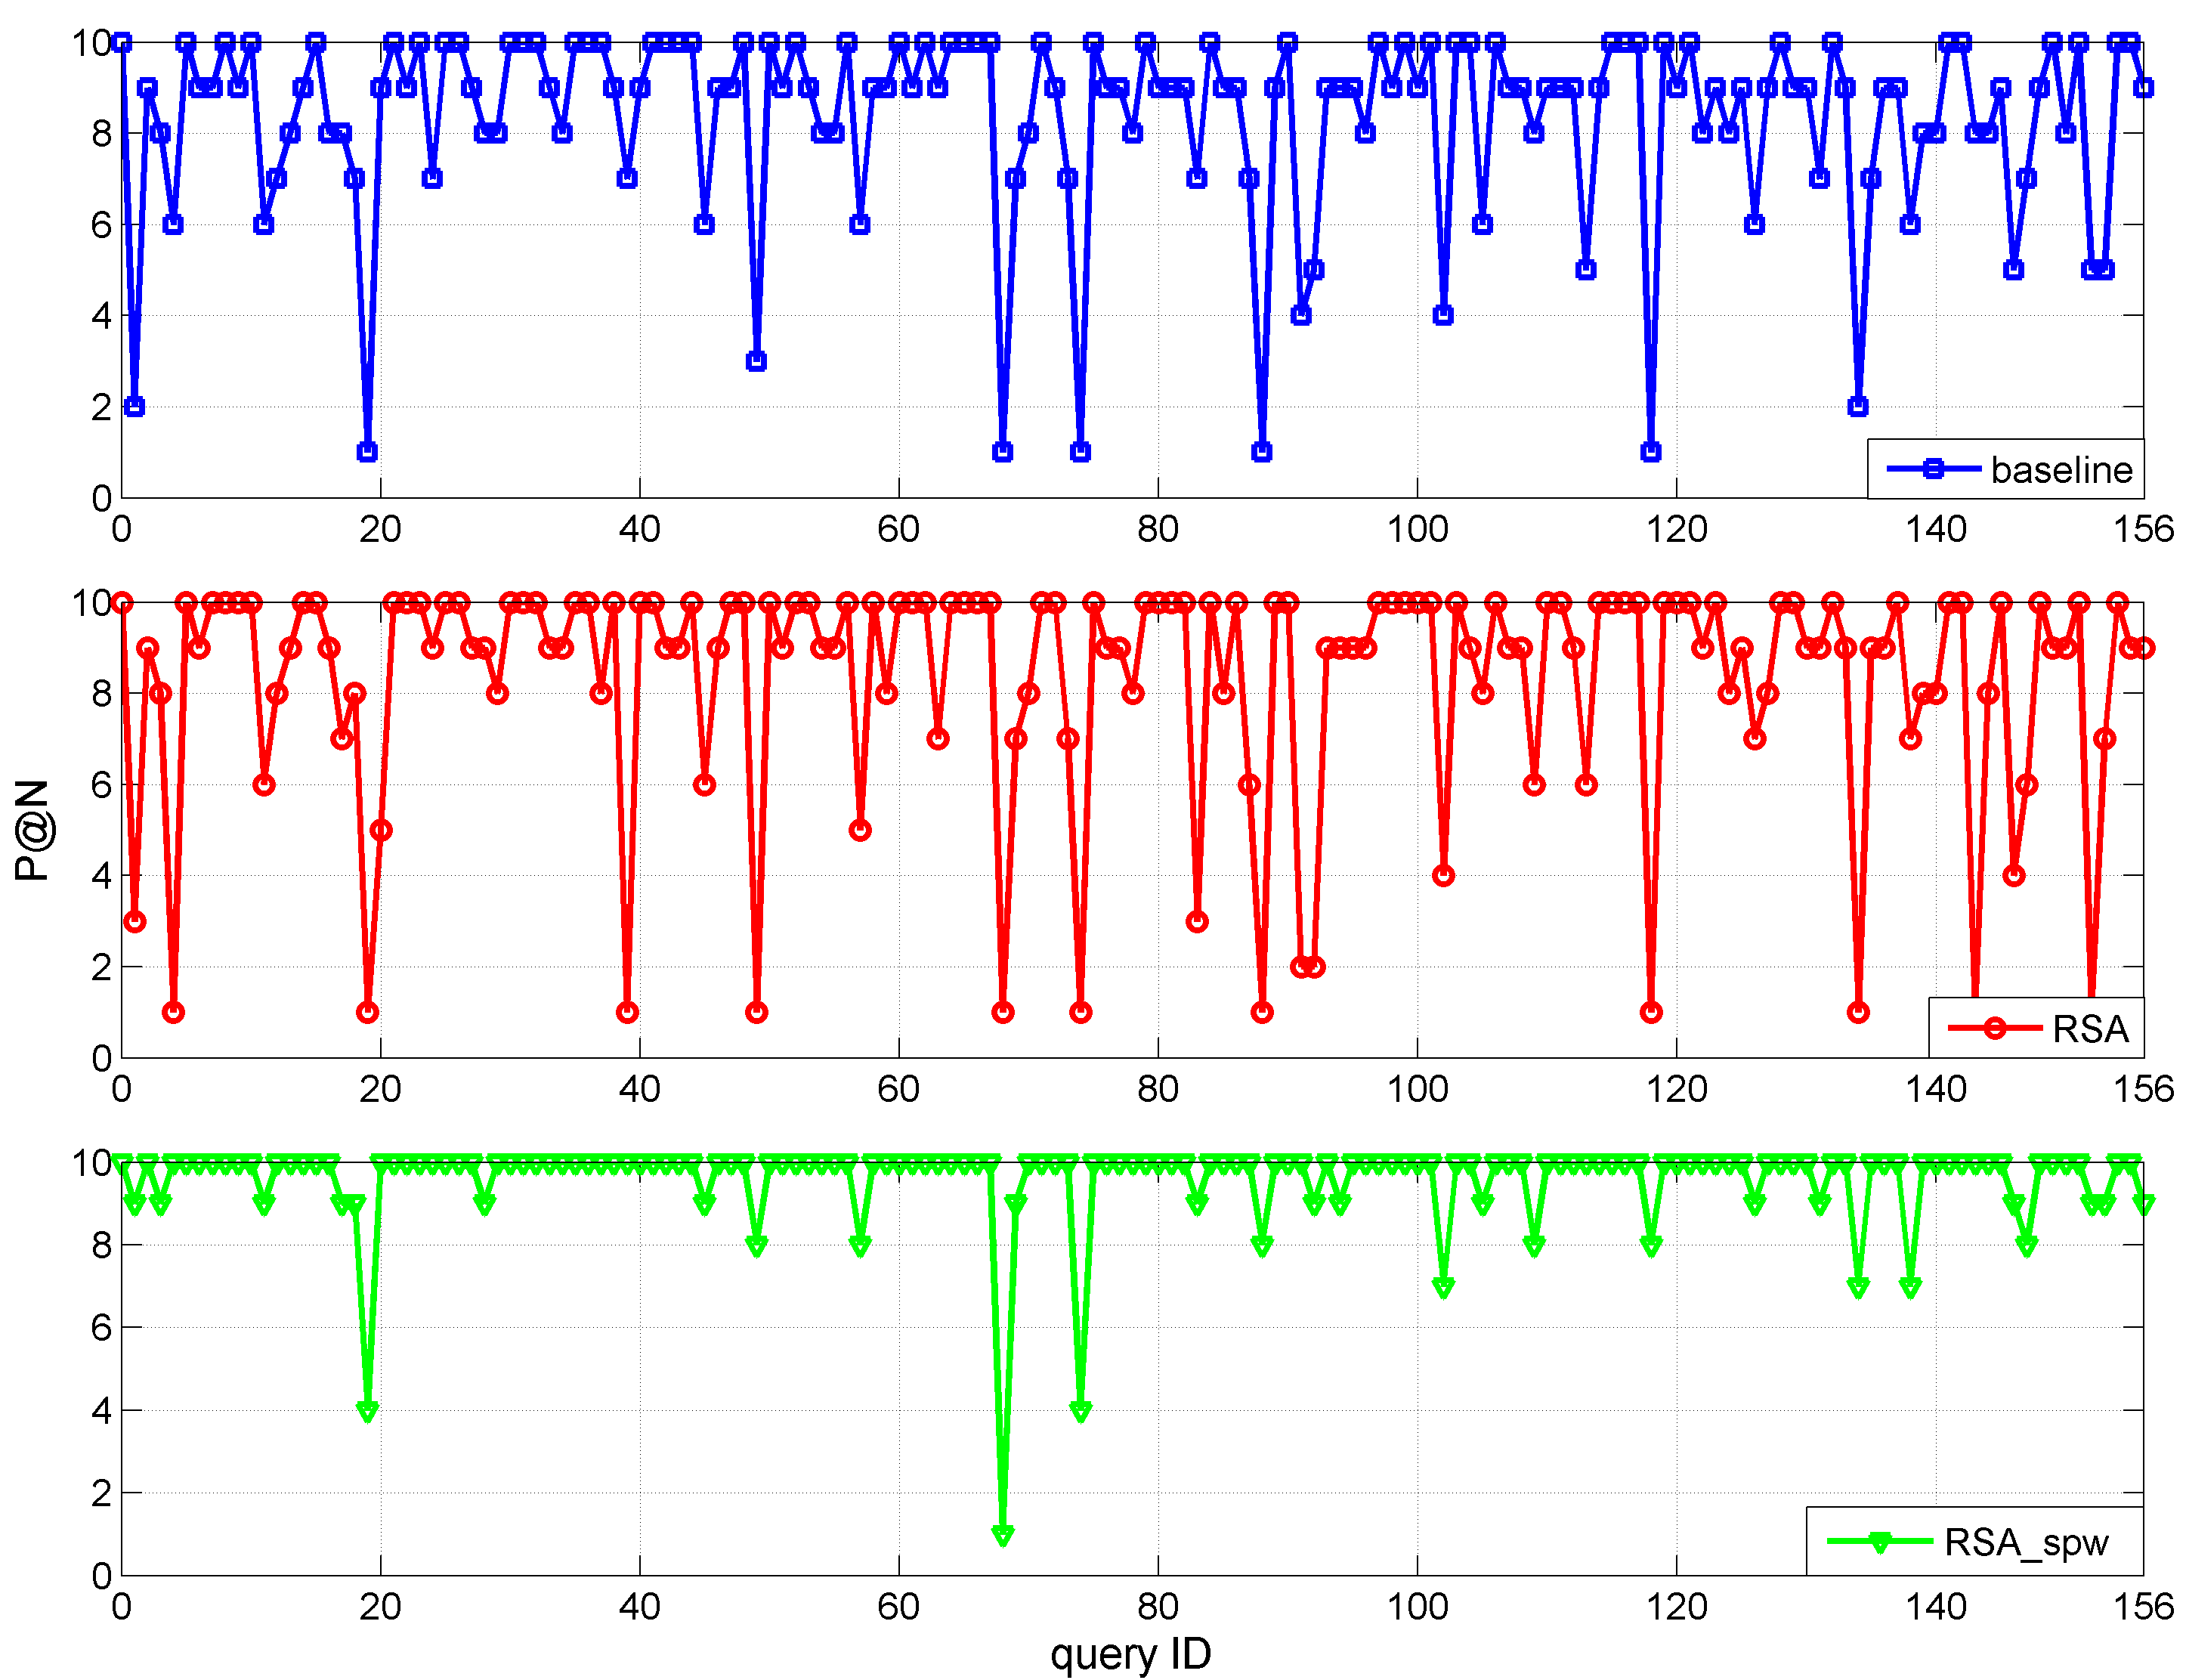
\includegraphics[width=0.8\textwidth]{scale.png}
	\caption{RSA算法在Copydays上的检索结果}\label{fig:rsa_s}
\end{figure}

\begin{figure}[h]
	\centering
	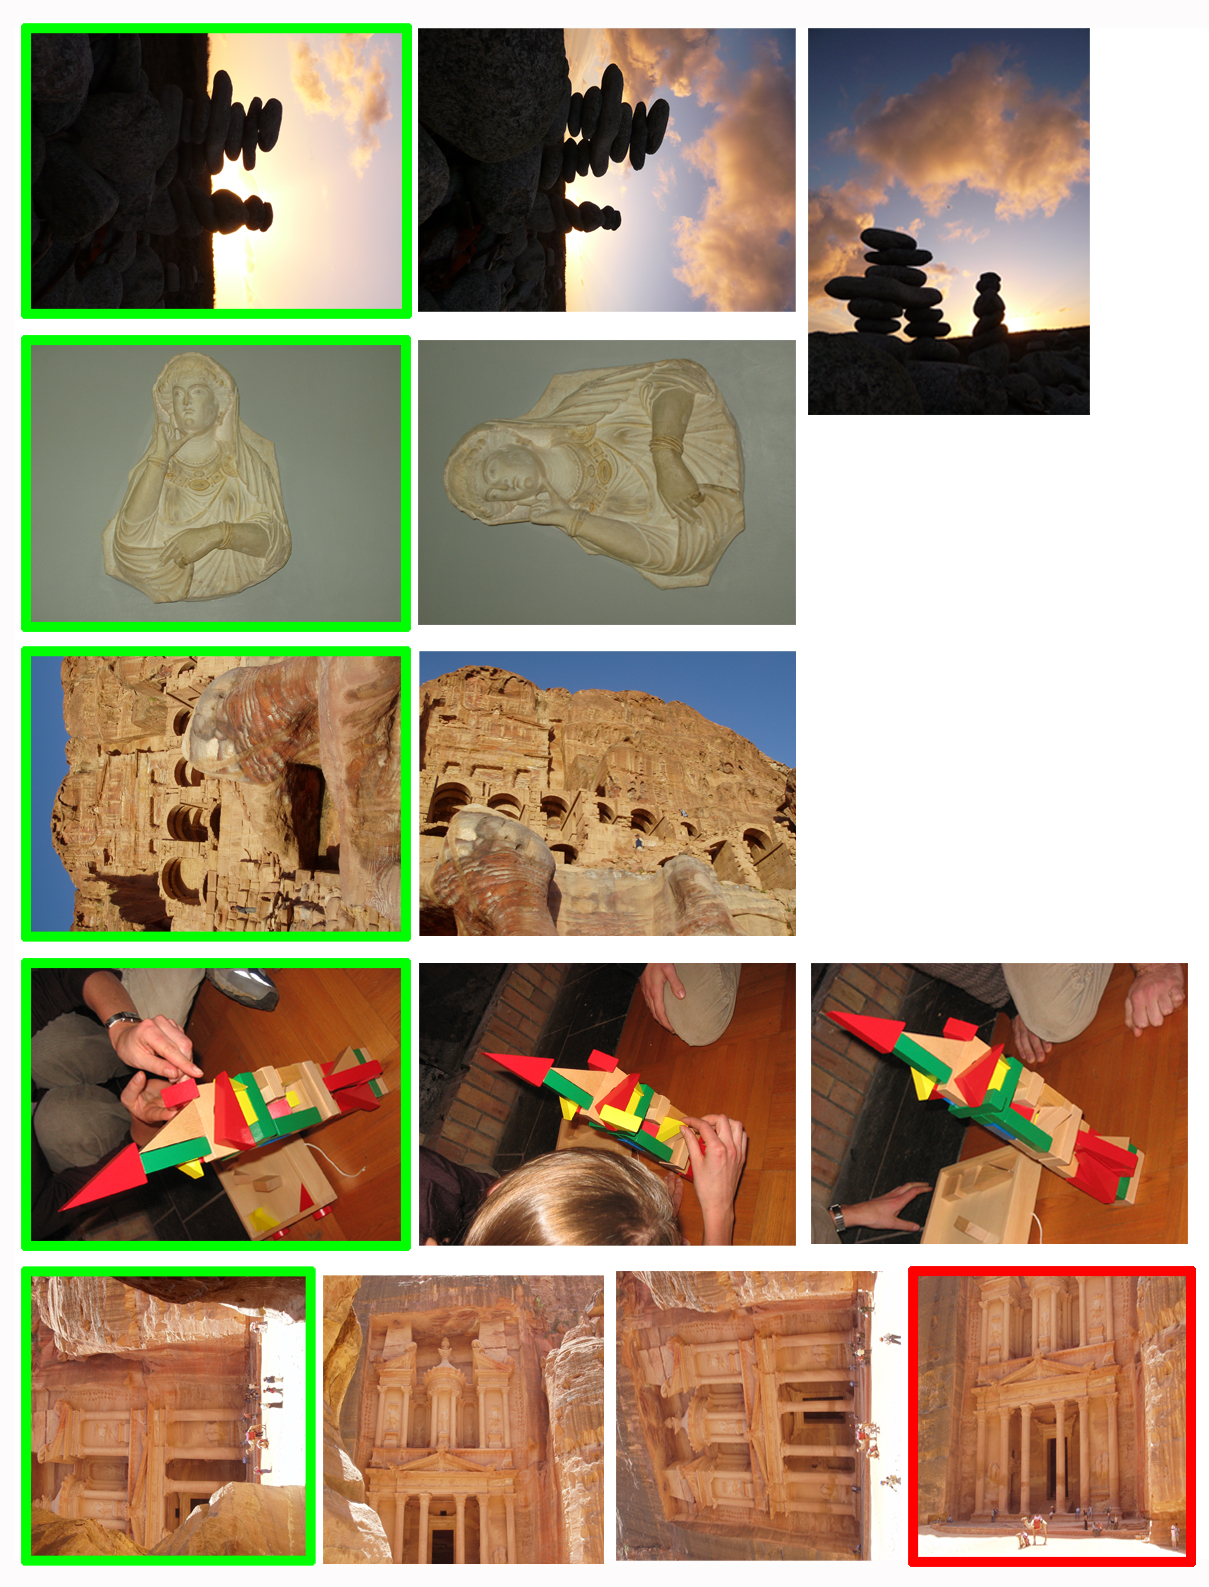
\includegraphics[width=0.8\textwidth]{rotation.jpg}
	\caption{RSA算法在Holidays上的检索结果}\label{fig:rsa_r}
\end{figure}

\section{本章小结}
本章节详细介绍了RSA算法。RSA算法可以明显的提高BoW图像检索的性能。RSA的核心思想是为图片建立Region Property Space(RPS),编码RPS中点的分布特性并在检索时对视觉单词进行几何校验。在RPS中的点具有两点特性:
\begin{enumerate}
	\item 具有明显的分布规律;
	\item 他们几乎不会出现在同一个位置上。
\end{enumerate}
基于第一个特性,我们提出了Spatial Weighting(SpW),SpW显著的提高的RSA的性能,而第二个特性保证了RSA可以对视觉单词进行较强的几何校验。通过量化,RSA在不影响检索效果的情况下占用了更少的内存。我们在三个标准数据集上对RSA算法进行了全面的测试。实验结果表明,RSA算法可以达到与state-of-the-art相近的检索精度。由于不需要后校验和先验知识,对尺度、角度变化不敏感,所以RSA适用于一般的大规模图像检索场景。





%\chapter{Main Orientation Net}

\section{引言}
在上一章我们详细介绍了RSA算法,RSA用来解决基于BoW图像检索框架中的几何校验问题。这一章将介绍Main Orientation Net(MONet),MONet用来解决现有基于CNN图像检索框架中无法很好解决图片旋转的问题。本章首先介绍相关研究工作,确定需要解决的问题;然后逐步介绍MONet的模型结构、模型参数和训练方案等;最后介绍基于CNN的图像检索框架,并通过实验证明MONet确实可以解决所提出的问题。


\subsection{相关工作}
\begin{figure}
	\centering
	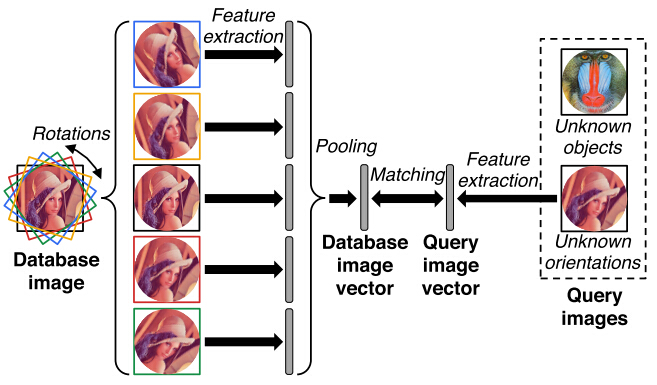
\includegraphics[width=\textwidth]{MaxPooling.jpg}
	\caption{使用MaxPooling解决图片旋转问题}\label{fig:maxpooling}
\end{figure}
在最初提出基于CNN的图像检索的工作\cite{babenko2014neural}中,对数据集中包含不同方向的图片做了两种简单的处理:
\begin{enumerate}
	\item 将所有图片旋转为正向;
	\item 或在训练时进行数据扩大,即将训练数据进行旋转($\pm90^{\circ}$)。
\end{enumerate}
以上两种方法虽然可以一定程度解决图片旋转的问题,但并不具有实用性。

\cite{chandrasekhar2015practical}提出了使用MaxPooling的方法,将不同方向的图片的特征进行融合,以达到对查询图片旋转的鲁棒性。\ref{fig:maxpooling}展示了使用MaxPooling融合图片特征并进行检索的过程。具体操作如下:
\begin{enumerate}
	\item 得到数据库图片的旋转的版本,旋转的范围为$-p^{\circ}$到$p^{\circ}$;
	\item 使用CNN网络得到所有图片(一张图片不同角度的副本)的特征;
	\item 使用MaxPooling将这些特征融合为一个特征,MaxPooling即保留这些特征向量每一维的最大值;
	\item 查询图片的处理和与数据图库片的相似度计算过程不变。
\end{enumerate}

通过CNN得到的图片特征是稀疏的,只有一些维度上有较大值:深度神经网络中对应节点产生的相应。正是由于CNN特征稀疏这一特点,才使得使用MaxPooling进行特征融合变为可能,MaxPooling保留了不同特征中的关键信息。虽然MaxPooling的方法可以很好的解决图片旋转的问题,但是其扩展性很差。第一,PCA降维方法不能与CNN特征结合使用;第二,该方案无法应用到传统的BoW图像检索框架中。在本章我们将提出不同的方案来解决图片旋转的问题,这种方法具有更好的扩展性,不影响原来的检索结构,也可以应用到传统的BoW框架中。

\section{图片方向}

\subsection{图片的梯度方向}
\begin{figure}
	\centering
	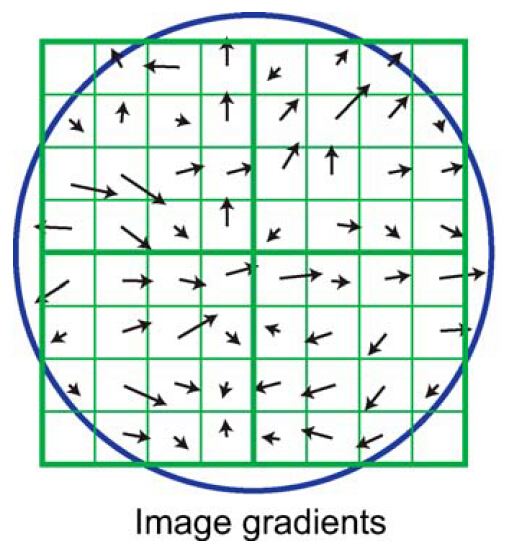
\includegraphics[width=0.5\textwidth]{gradient.jpg}
	\caption{图片区域梯度方向示意图}\label{fig:gradient}
\end{figure}
在介绍图片主方向之前,我们先介绍计算机视觉中经常遇到的一个相似的概念:图片的梯度方向。令$L(x,y)$表示一个像素的坐标,则图片的梯度方向由相邻像素之间的梯度大小$m(x,y)$和方向$\theta(x,y)$共同决定:
\begin{equation}
m(x,y) = \sqrt{(L(x+1,y)-L(x-1,y))^2 + L(x,y+1)-L(x,y-1))^2}
\end{equation}
\begin{equation}
\theta(x,y)=\tan^{-1}\frac{L(x,y+1) - L(x,y-1)}{L(x+1,y) - L(x-1,y)}
\end{equation}

图\ref{fig:gradient}为一个图片区域的梯度方向示意图。梯度方向有很多应用,比如构建具有旋转不变性的描述符\cite{lowe2004distinctive}。但是,我们却无法用梯度方向来描述一幅图像的方向。这是由于在一副自然图片中,梯度方向的分布是接近均匀分布的,这一点也可以从图\ref{fig:RSA_dis_2}(c)中得到。所梯度方向往往应用于一块blob区域。

\subsection{图片的主方向}
由于拍摄时选取的角度问题,或者是人为修改,在进行图片检索时,查询图片(包括数据库图片)可能不是竖直的。而图片旋转会为图像检索带来不小的困难,在使用几何校验算法时由甚\cite{jegou2008hamming}\cite{lazebnik2006beyond}。在使用CNN的图像检索框架时,由于CNN提取的是图片的全局特征,图片旋转的问题将更为突出。为此,我们训练了一个学习图片主方向的网络Main Orientation Net(MONet)。

\begin{figure}
	\centering
	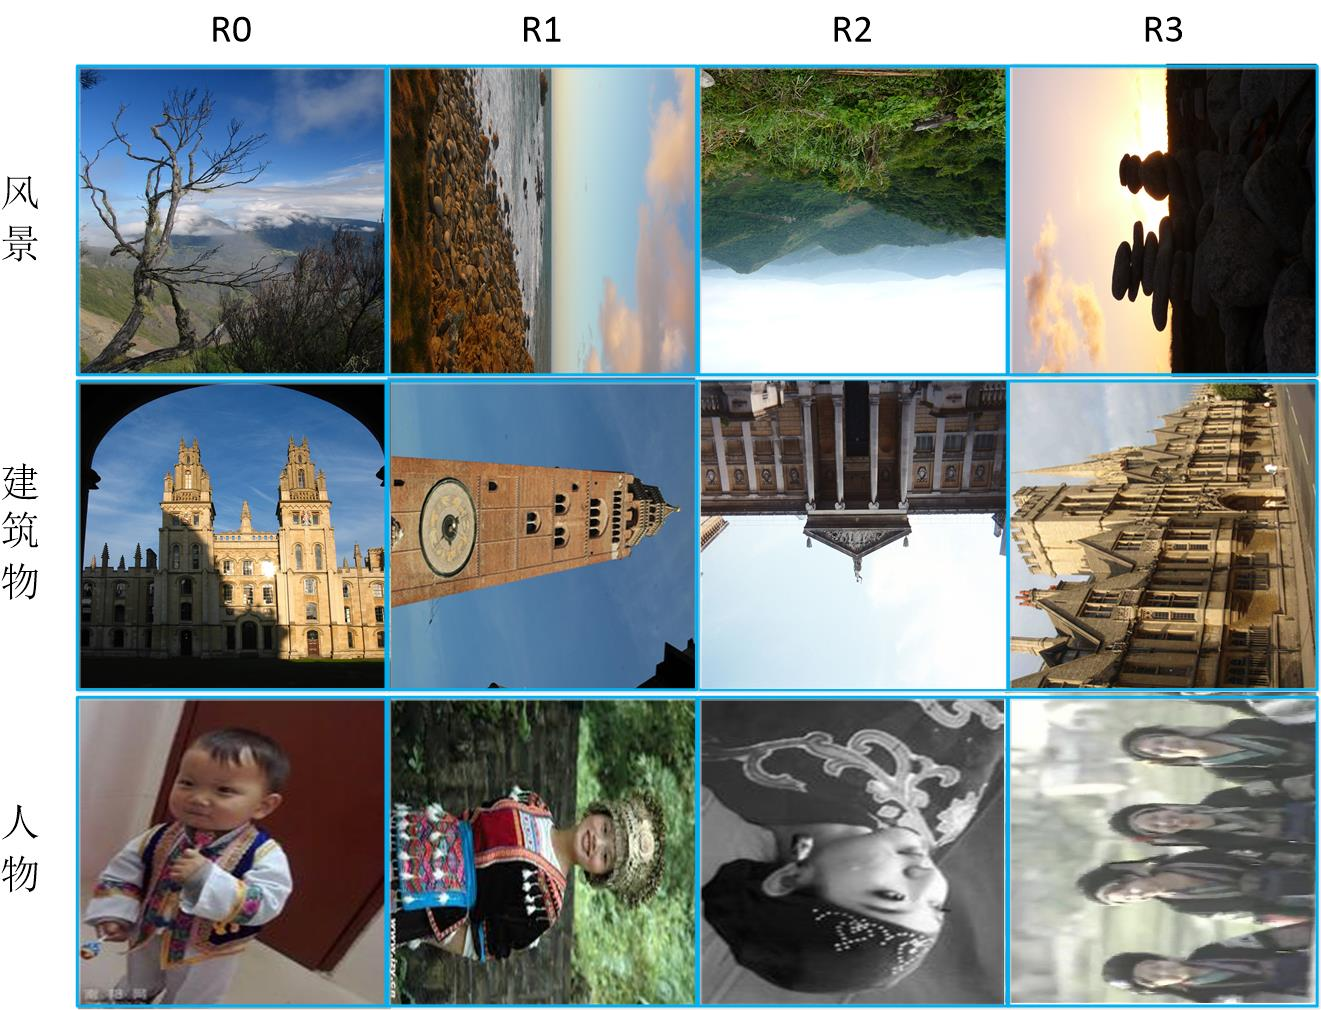
\includegraphics[width=0.8\textwidth]{Main_Orientation.jpg}
	\caption{不同主方向的自然图片}\label{fig:main_ori}
\end{figure}

我们定义图片的主方向为图片中垂直于地表的方向,为了简化问题,我们认为在图像检索中图片只存在4中方向,即$0^{\circ}$、$90^{\circ}$、$180^{\circ}$和$270^{\circ}$,分别表示为$R0$,$R1$,$R2$和$R3$。图\ref{fig:main_ori}给出了风景、建筑物和人物在不同主方向下的情况。对于图\ref{fig:main_ori}中的情况,人很容易判断图片的主方向,我们希望MONet同样可以判断出图片的主方向。

\begin{figure}
	\centering
	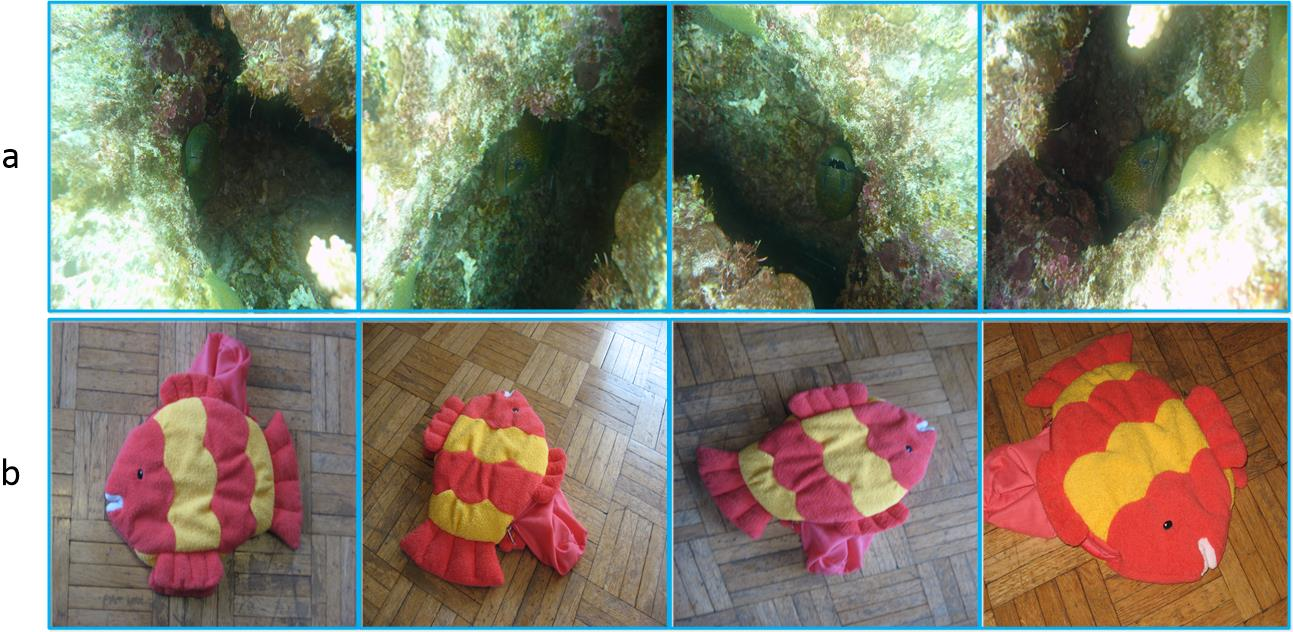
\includegraphics[width=0.8\textwidth]{None_MO.jpg}
	\caption{不容易确定主方向的自然图片}\label{fig:n_mo}
\end{figure}

在有些情况下,图片的主方向是不容易确定的。如图\ref{fig:n_mo}所示,其中(a)中的鱼不明显,所以很难判断图片的主方向;(b)中图片的方向并不重要,可以认为没有主方向。对于以上情况,MONet也是不予考虑的。

\section{图片主方向对检索的影响}
\begin{figure}
	\centering
	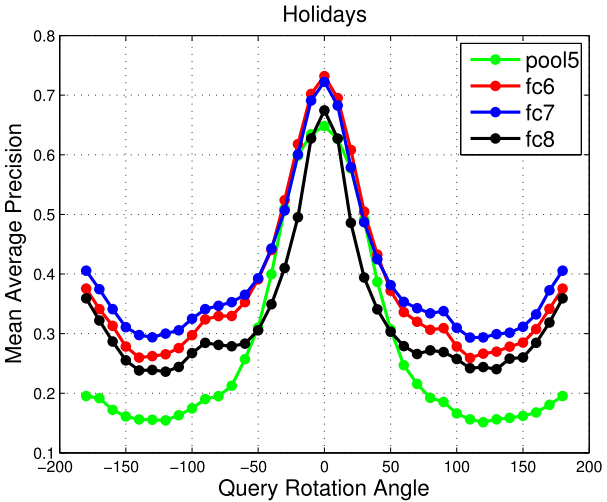
\includegraphics[width=0.7\textwidth]{Holidays_r.jpg}
	\caption{查询图片旋转对CNN检索框架的影响}\label{fig:hr}
\end{figure}
为了测试图片旋转对基于CNN的图像检索框架的影响,我们使用了2.3节介绍的框架进行旋转情况下的图像检索实验。图\ref{fig:hr}显示了不同旋转角度下的查询结果,其中横轴表示查询图片旋转的角度(从$-180^{\circ}$到$+180^{\circ}$),纵轴表示检索结果(用mAP表示),不同的曲线表示使用不同层的CNN特征。通过实验结果可以看出,查询图片的旋转对检索精度有很大的影响,当图片旋转$10^{\circ}$时,mAP就有明显的下降。可以想象,网络上存在的大量的经过旋转的图片将会对CNN图像检索框架产生严重的影响。

\section{MONet网络设计}
在设计MONet时,我们主要考虑了以下几点问题:
\begin{enumerate}
	\item MONet学习图片的主方向,而不关注图片的细节,所以该网络应该有更小的图片输入和更大的卷积核;
	\item 网络应该具有稀疏性,提高训练速度并减少参数量;
	\item 可以从MONet中方便的提取特征,用于后续处理;
	\item 在应用MONet时,可以快速的判断图片的主方向,保证图片检索的速度。
\end{enumerate}

我们借鉴了GoogLeNet中Inception\cite{szegedy2015going}的思想,设计了MONet的模型如图\ref{fig:monet_f}所示。其中,虚线框出的结构就是一个Inception\cite{szegedy2015going},Inception用稠密的网络结构模拟了稀疏网络结构,减少了参数量的同时提高了运行速度,并且Inception还完成的多尺度的识别,保证了模型的识别能力。

\begin{figure}
	\centering
	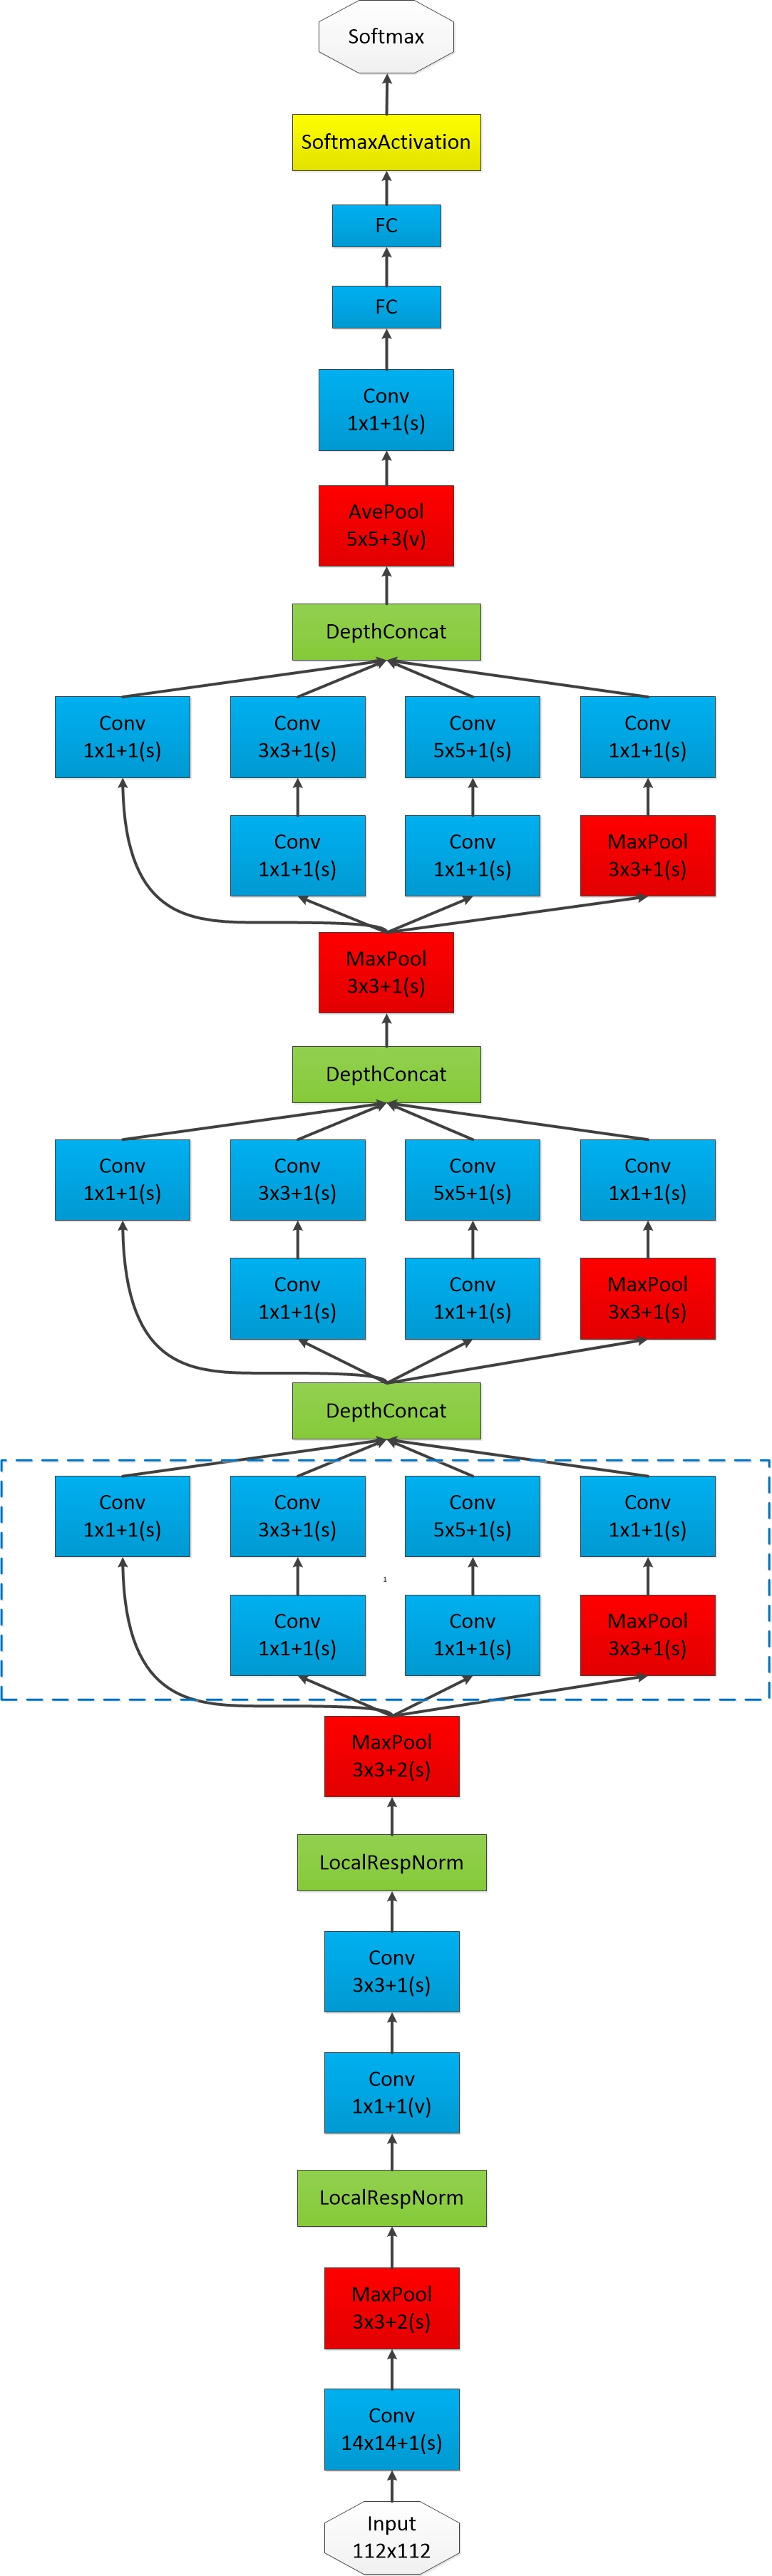
\includegraphics[width=0.43\textwidth]{MONet_frame.jpg}
	\caption{MONet框架图}\label{fig:monet_f}
\end{figure}

表\ref{tab:monet}列出了MONet各层的参数。其中,$x\times x$ reduce表示在进行$x\times x$卷积前进行的削参操作,pool proj表示在进行pooling操作之前进行的投影操作,目的是减少feature map的个数。
\begin{table}
	\begin{center}
		\begin{tabular}{|c|c|c|c|c|c|c|c|c|}
			\hline
			type & patch size & $1\times1$ & $3\times3$ & $3\times3$ & $5\times5$ & $5\times5$ & pool & params \\
			     & /stride    &            & reduce     &            &            &     reduce & proj &        \\
			\hline
			\hline
			conv & $14\times14/1$ & & & & & & & 11K\\
			\hline
			max  & $3\times3/2$ & & & & & & & \\
			\hline
			conv & $3\times3/1$ & & 64 & 192 & & & & 112K\\
			\hline
			max  & $3\times3/2$ & & & & & & &\\
			\hline
			incep(a) & & 64 & 96 & 128 & 16 & 32 & 32 & 159K\\
			\hline
			incep(b) & & 128 & 128 & 192 & 32 & 96 & 64 & 380K\\
			\hline
			max  & $3\times3/2$ & & & & & & &\\
			\hline
			incep(c) & & 192 & 96 & 208 & 16 & 48 & 64& 364K\\
			\hline
			ave & $5\times5/3$ & & & & & & &\\
			\hline
			fc(a) & & & & & & & & 8M\\
			\hline
			fc(b) & & & & & & & & 4K\\
			\hline
		\end{tabular}
	\end{center}
	\caption{MONet各层参数}
	\label{tab:monet}
\end{table}


\section{MONet网络训练}
由于训练数据有限,我们假设图片只有四个主方向,即$R0$,$R1$,$R2$和$R3$。这种假设也是合理的,因为在实际的图片库中,绝大多数的图片只有这四种主方向,而不会出现任意方向的旋转。为了保证MONet的可扩展性,我们在不同的数据集上进行训练和测试,同时这两个数据集最好有一定的相关性。所以在我们的实验中,我们用Paris\cite{philbin2008lost}上进行训练,在Oxford5K\cite{philbin2007object}进行测试。我们将图片主方向的学习过程认为是图片分类问题,具体流程如下:
\begin{enumerate}
	\item 图片预处理:分别将Paris和Oxford5K中的图片进行旋转,旋转后的角度($Rx$)即为图片的标签;
	\item 使用GoogLeNet在ILSVRC上的训练结果作为MONet的权重初值;
	\item 配置网络结构,并使用Paris进行训练(相当于fine-tune);
	\item 使用Oxford5K测试网络的性能;
	\item 后处理:包括PCA降维和SVM分类等。
\end{enumerate}

我们将batch大小设为32张图片,每500次迭代进行一次测试,两万次的迭代的结果如图\ref{fig:monet_t}所示,其中横轴为迭代次数,纵轴为准确率。可以看出当迭代2000次时,MONet的准确率基本达到峰值,我们将迭代两千次的网络作为后续试验的基本模型。

\begin{figure}
	\centering
	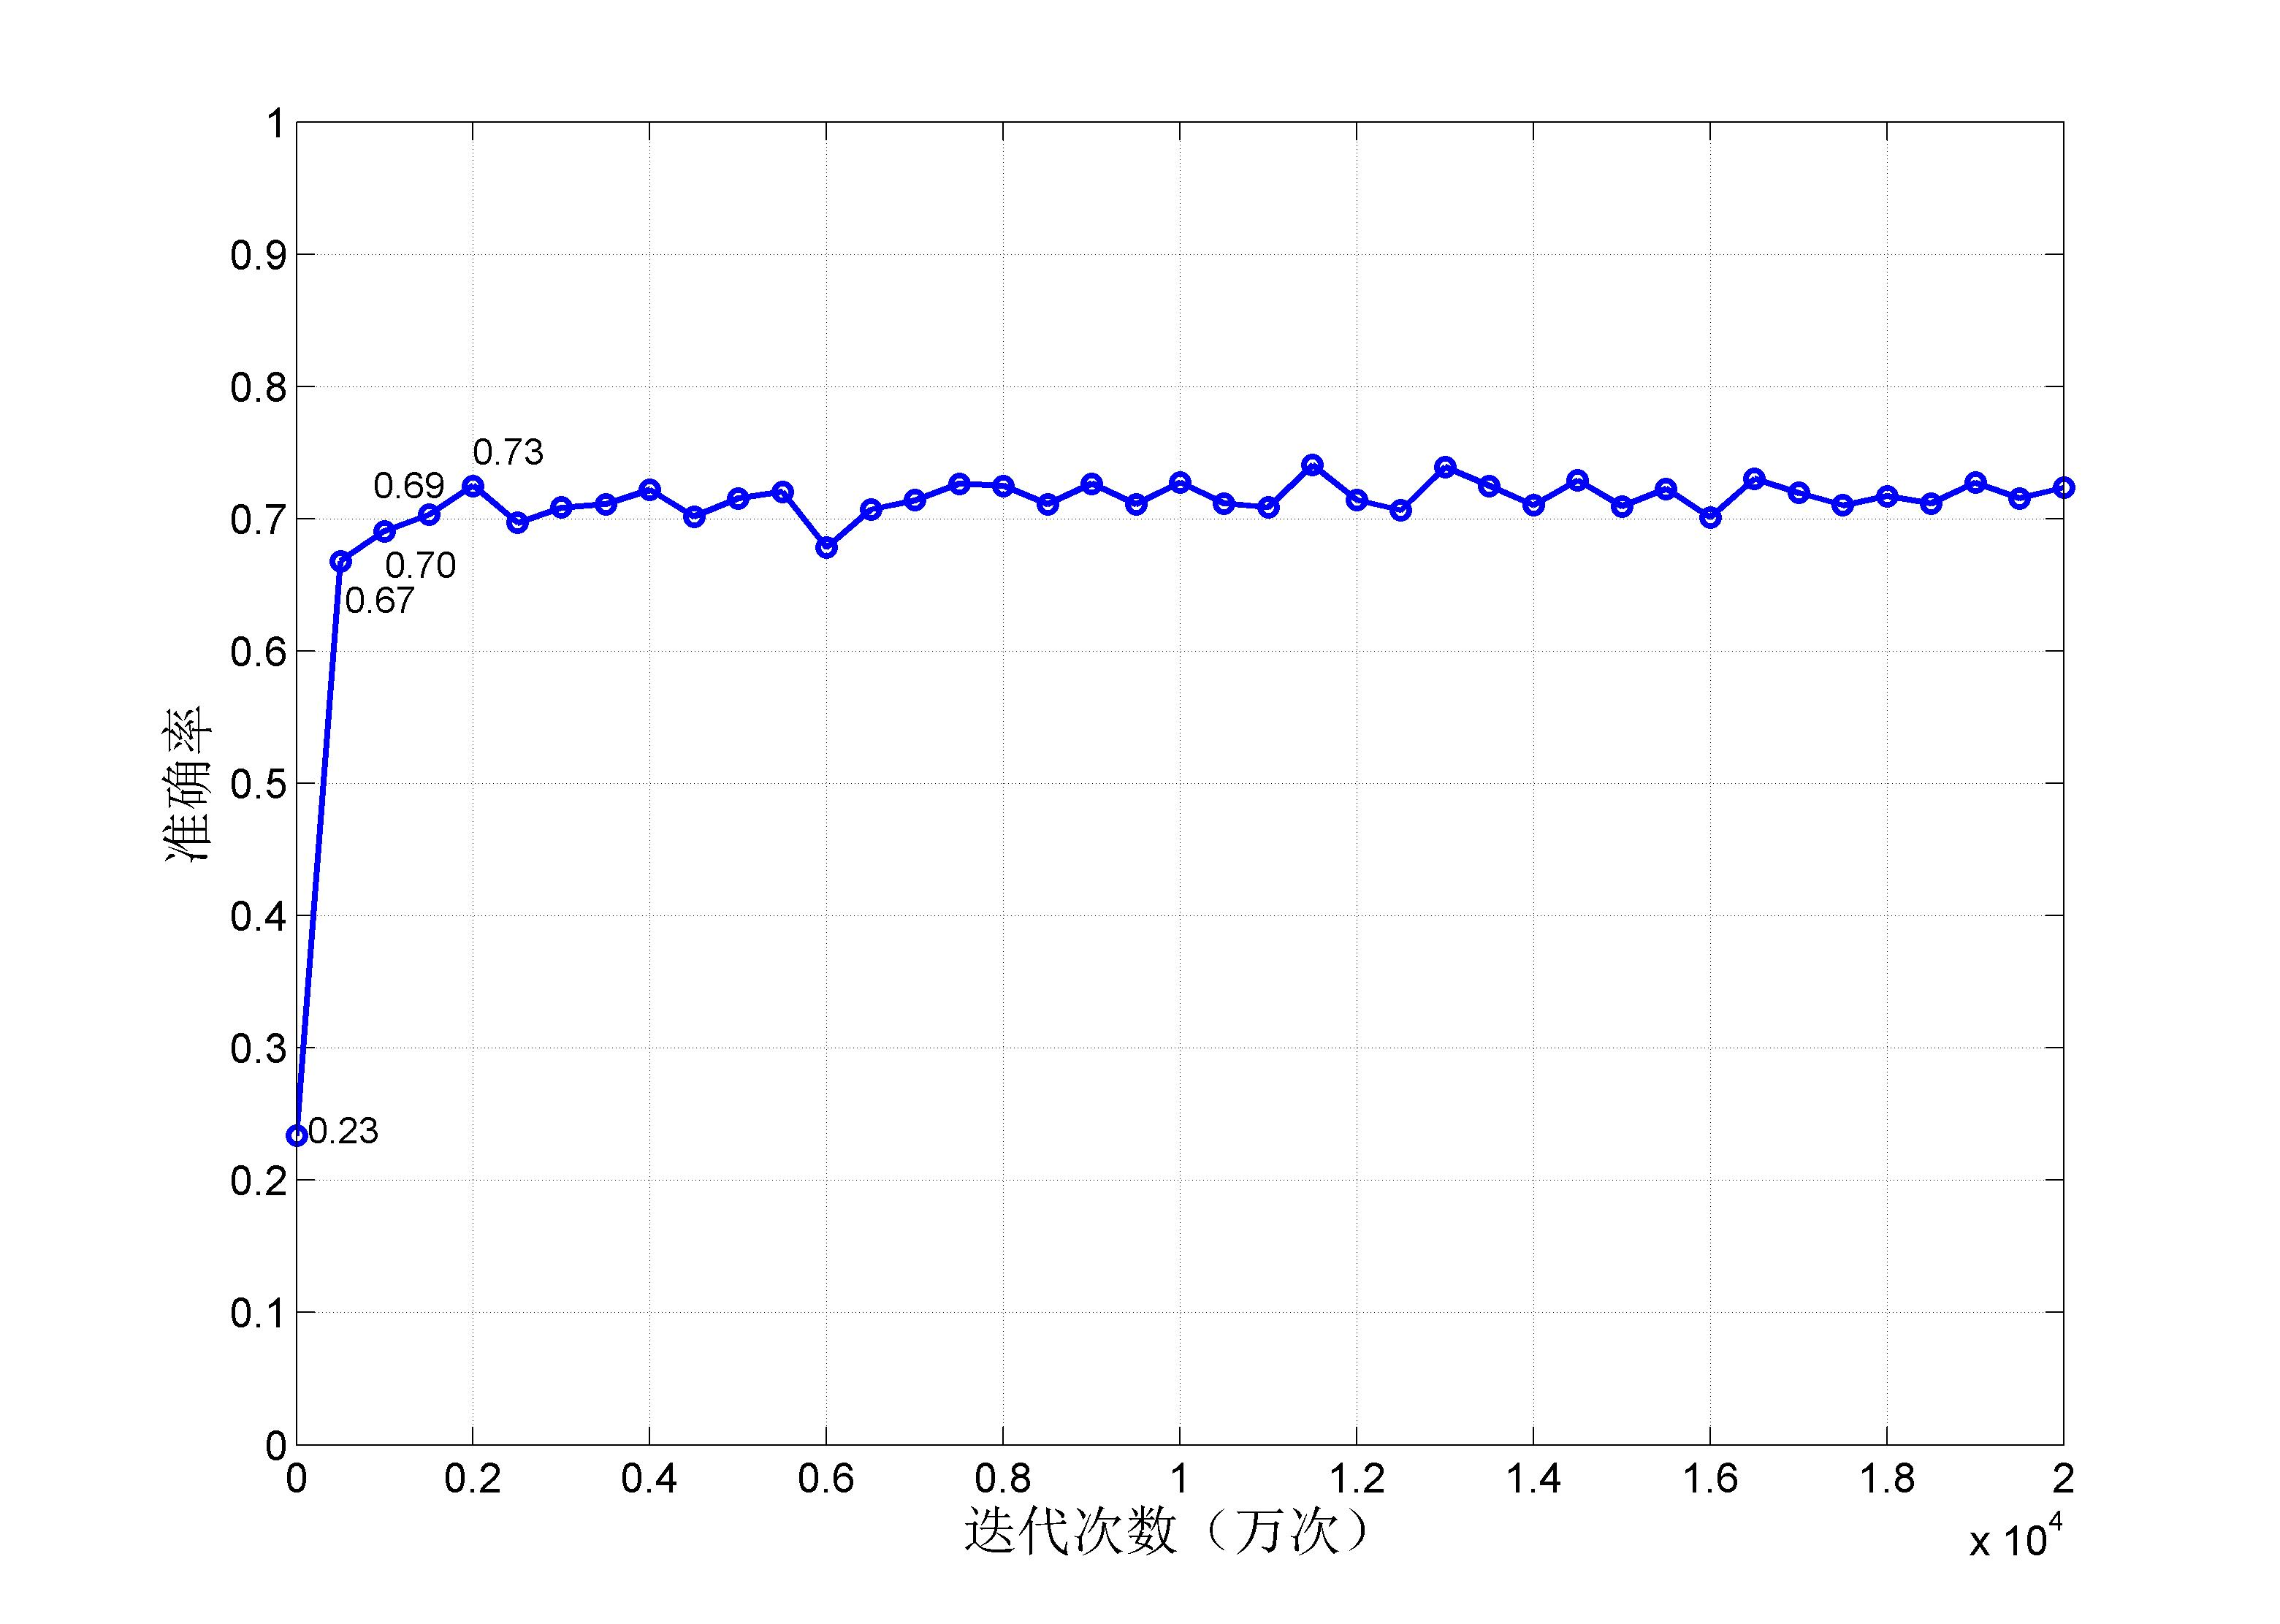
\includegraphics[width=0.7\textwidth]{MONet_train.jpg}
	\caption{MONet训练过程中的准确率变化情况}\label{fig:monet_t}
\end{figure}

为了进一步提高MONet的分类准确率,我们在MONet之后增加了一个SVM分类器。SVM分类器的输入为Paris图片的CNN特征(fc(a)层输出,1024维)和图片的主方向($Rx$),训练数据为Oxford5K的CNN特征。在添加SVM分类器后,MONet的准确率提高到0.810。最终,MONet的正整体结构如图\ref{fig:monet_ff}所示。

\begin{figure}
	\centering
	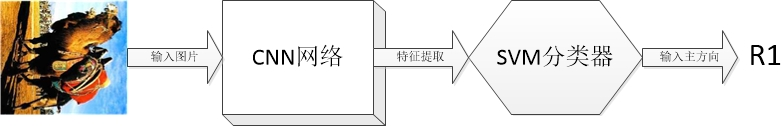
\includegraphics[width=0.9\textwidth]{MONet_frame_f.jpg}
	\caption{MONet整体结构}\label{fig:monet_ff}
\end{figure}

\section{CNN图像检索框架}
使用MONet进行图片检索是非常容易的,只需要将MONet作为查询图片的预处理步骤即可。这也是MONet的优点之一,可以方便的与现有的图像检索模型融合。使用CNN网络的图片检索整体框架如图\ref{fig:cnn_rf}所示,第一个CNN网络为MONet,用来判断图片的主方向;第二个CNN网络用于提取图片特征,完成相似度计算。

\begin{figure}
	\centering
	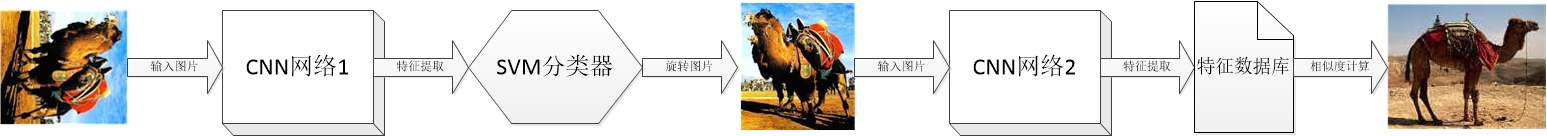
\includegraphics[width=\textwidth]{CNN_retrieval_frame.jpg}
	\caption{基于CNN的图像检索整体框架}\label{fig:cnn_rf}
\end{figure}

\section{实验}
我们针对相似图像检索任务对MONet的效果进行了测试。

\subsection{实验模型}
我们的实验模型主要由两部分组成,包括用于判断图片主方向的MONet和提取图片特征的AlexNet。模型整体框架如图\ref{fig:cnn_rf}所示。Baseline模型为不使用MONet进行处理的AlexNet,改进模型为经过旋转预处理的MONet,其实验结果分别标记为“AlexNet”和“MONet”。

\subsection{实验数据}
与训练MONet一样,我们进行测试时同样使用了Paris\cite{philbin2008lost}训练MONet,使用Oxford 5K\cite{philbin2007object}测试检索的性能。这主要是考虑了Paris和Oxford5K之间的相关性,即这两个数据库都只包含了建筑物,并且没有交集。Oxford数据集中的图片都是竖直的($R0$),因此我们将每个查询图片都生成4张不同主方向的图片,分别表示为$R0$、$R1$、$R2$和$R3$,并测试在不同主方向下的检索结果。

\subsection{图片特征}
在检索时,我们提取图片的四种特征,分别为AlexNet的Pooling 5层特征(9216维)、fully connected 6层特征(4096维)、fully connected 7层特征(4096维)和输出层特征(1000维)。图片的这些特征分别简记为“pool5”、“fc6”、“fc7”和“fc8”。

\subsection{实验结果}
\begin{figure}
	\centering
	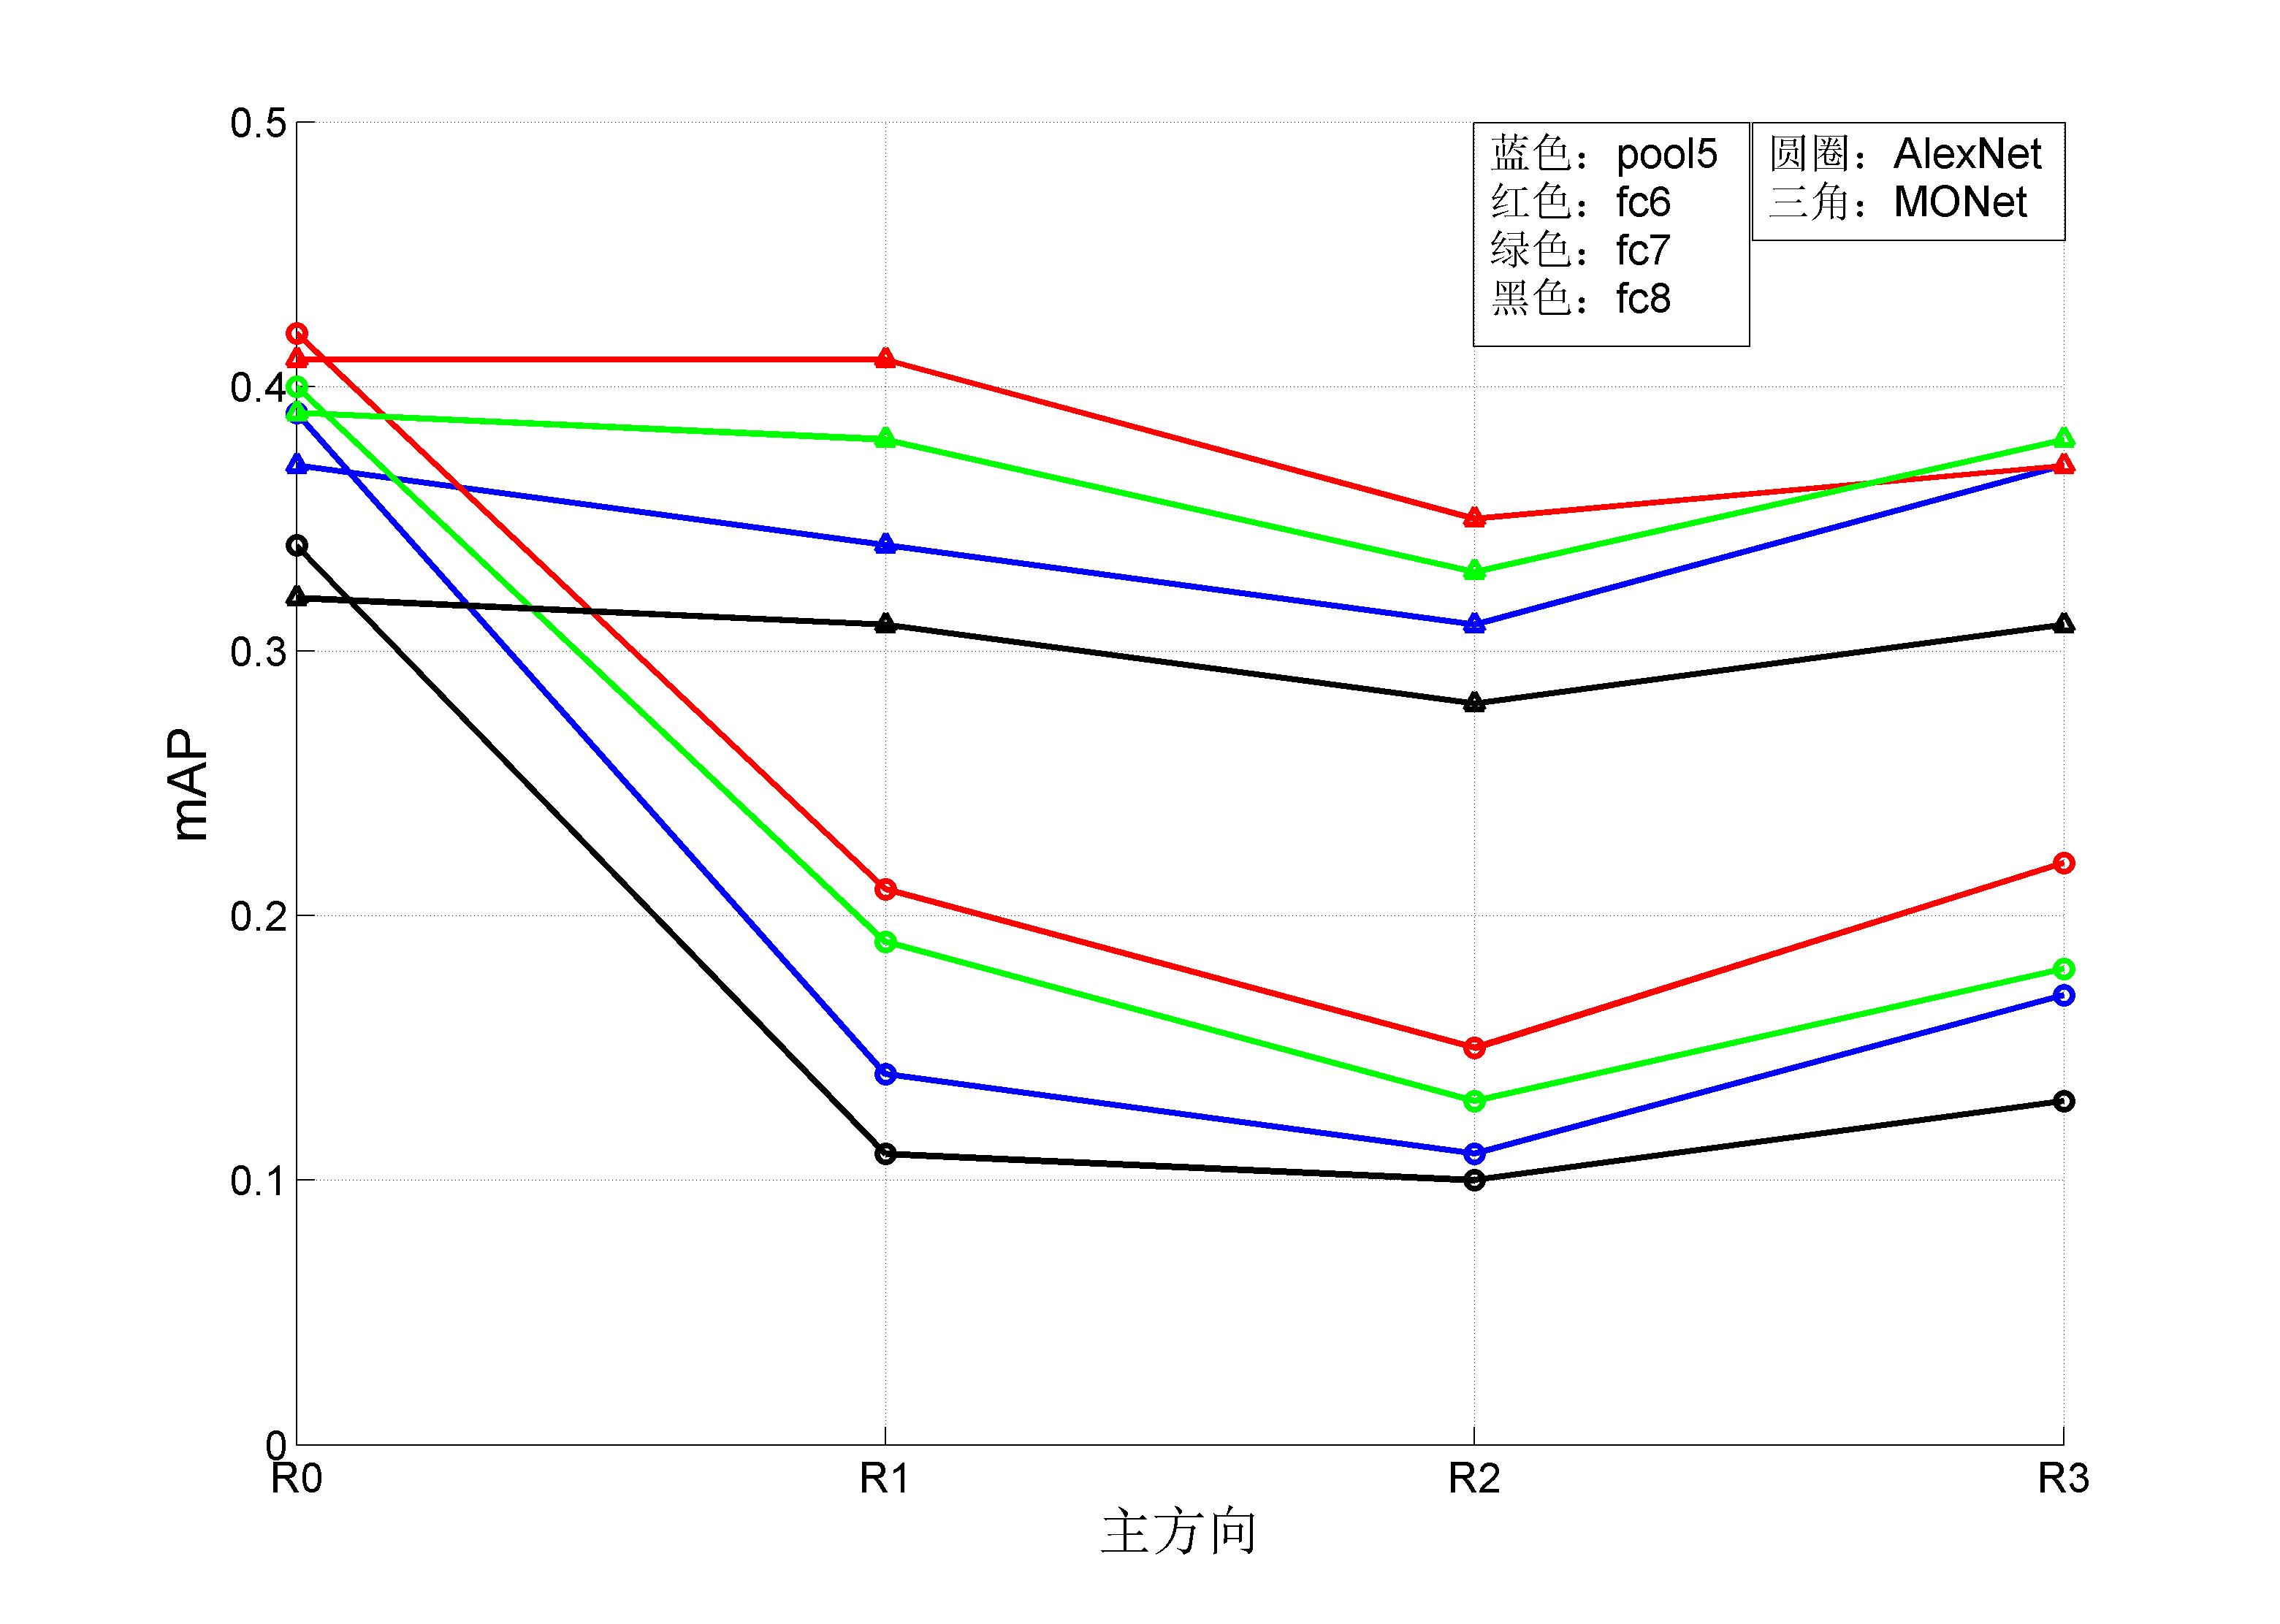
\includegraphics[width=0.8\textwidth]{MONet_res.jpg}
	\caption{MONet在Oxford5K数据集上的检索结果}\label{fig:monet_r}
\end{figure}
实验结果如图\ref{fig:monet_r}所示。其中,不同颜色的曲线表示使用AlexNet网络中不同层的特征,圆圈表示没有进行MONet预处理,三角表示进行MONet预处理后的结果。从图\ref{fig:monet_r}中可以看出,在图片旋转时,AlexNet网络的检索性能会显著下降,而经过MONet的预处理后,可以保证不同主方向的图片都可以有较好的检索结果。


\section{MONet的应用}
MONet对图片进行预处理,所以这个网络可以应用于任何的图片预处理步骤,本节就介绍MONet的两个应用。

\subsection{BoW框架下MONet的应用}
由于局部特征一般具有旋转不变性(例如SIFT\cite{lowe2004distinctive}),所以基于BoW框架的图像检索可以很好的应对图片旋转的问题。但是,正如2.5节中提到的现有的很多几何校验算法无法解决图片旋转的问题:\cite{philbin2007object}中的FSM和\cite{lazebnik2006beyond}中的SPM要求图片必须是竖直的;\cite{jegou2008hamming}中的WGC需要图片方向的先验知识。图片主方向的问题限制了很多几何校验算法的应用场景,而MONet可以很好的解决这个问题。

为了验证MONet对传统的BoW框架中的几何校验有帮助,我们做了如下对比实验:
\begin{enumerate}
	\item 使用经典的BoW框架和FSM\cite{philbin2007object}几何校验作为baseline,记作$R0$;
	\item 将查询图片进行$90^{\circ}$、$180^{\circ}$和$270^{\circ}$的旋转,并进行上述相同的实验,记作$R1$、$R2$和$R3$;
	\item 将查询图片进行$90^{\circ}$、$180^{\circ}$和$270^{\circ}$的\textbf{随机}旋转,并使用MONet进行预处理,再进行上述实验,记作MONet。
\end{enumerate}

通过上述实验设置,我们得到了表\ref{tab:monet_bow}的结果,其中每行表示Oxford5K中的一类建筑物,每列为不同的旋转和方法,结果为相应建筑物检索的mAP。通过表\ref{tab:monet_bow}可以看出,虽然BoW框架对图像的旋转有一定的鲁棒性,但是几何校验一般需要假设图片的主方向,所以当查询图片旋转时,检索精度有一定的下降;通过MONet的预处理(将超过80\%的图片旋转为正向),可以得到与不进行旋转情况相近的结果。通过以上结果可以得出结论,MONet可以与传统的BoW框架结合使用,使其更加对图片旋转更加鲁棒。
\begin{table}
	\begin{center}
		\begin{tabular}{|c|c|c|c|c|c|}
			\hline
						& $R0$  & $R1$ & $R2$ & $R3$ & MoNet \\
			\hline
			all\_souls	& 79.75 & 68.60 & 68.57 & 68.05 & 78.03\\
			\hline
			ashmolean   & 63.89 & 45.44 & 46.23 & 46.03 & 64.33\\
			\hline
			balliol     & 77.79 & 78.15 & 77.50 & 77.95 & 77.09\\
			\hline
			bodleian    & 90.61 & 79.55 & 79.62 & 80.41 & 91.44\\
			\hline
			christ\_church&64.91 & 60.91& 61.03 & 60.99 & 64.82\\
			\hline
			cornmarket  & 65.87 & 47.13 & 45.86 & 46.69 & 64.63\\
			\hline
			hertford    & 88.34 & 84.35 & 84.84 & 85.32 & 88.29\\
			\hline
			keble       & 93.70 & 83.69 & 83.80 & 83.98 & 94.04\\
			\hline
			magdalen    & 29.71 & 24.04 & 24.07 & 24.84 & 29.83\\
			\hline
			pitt\_rivers& 100.0 & 97.77 & 97.55 & 97.37 & 100.0\\
			\hline
			radcliffe\_camera& 77.41 & 74.38 & 74.27 & 73.69 &76.88\\
			\hline
			mAP         & 75.63 & 67.63 & 67.57 & 67.75 & 75.40\\
			\hline
		\end{tabular}
	\end{center}
	\caption{MONet与传统BoW框架结合的检索结果}
	\label{tab:monet_bow}
\end{table}

\subsection{服饰检测中MONet的应用}

基于MONet和CNN分类网络,我们设计了一个服饰检测系统,CostumeNet。CostumeNet用来识别图片中人物所穿服饰所属的民族。首先我们收集了两个数据集,用来测试和训练CostumeNet,分别为Costume-12和Costume-38。

\subsubsection{Costume-12数据集}
Costume-12为从网络上下载的12个中国少数民族服饰的数据集。这12个少数民族包括:白族、布依族、朝鲜族、傣族、俄罗斯族、回族、满族、蒙古族、苗族、维族、彝族和藏族。每一类包含约300张图片,共3635张图片。由于这些图片全部来自网络,可能存在错误,即图片中不包含相应类别的服饰,或服饰类别错误。绝大多数图片中包含人,即人穿着相应的民族服饰,部分图片可能是衣服、首饰甚至漫画。图\ref{fig:costume-12}展示了Costume-12中的部分图片。

\begin{figure}
	\centering
	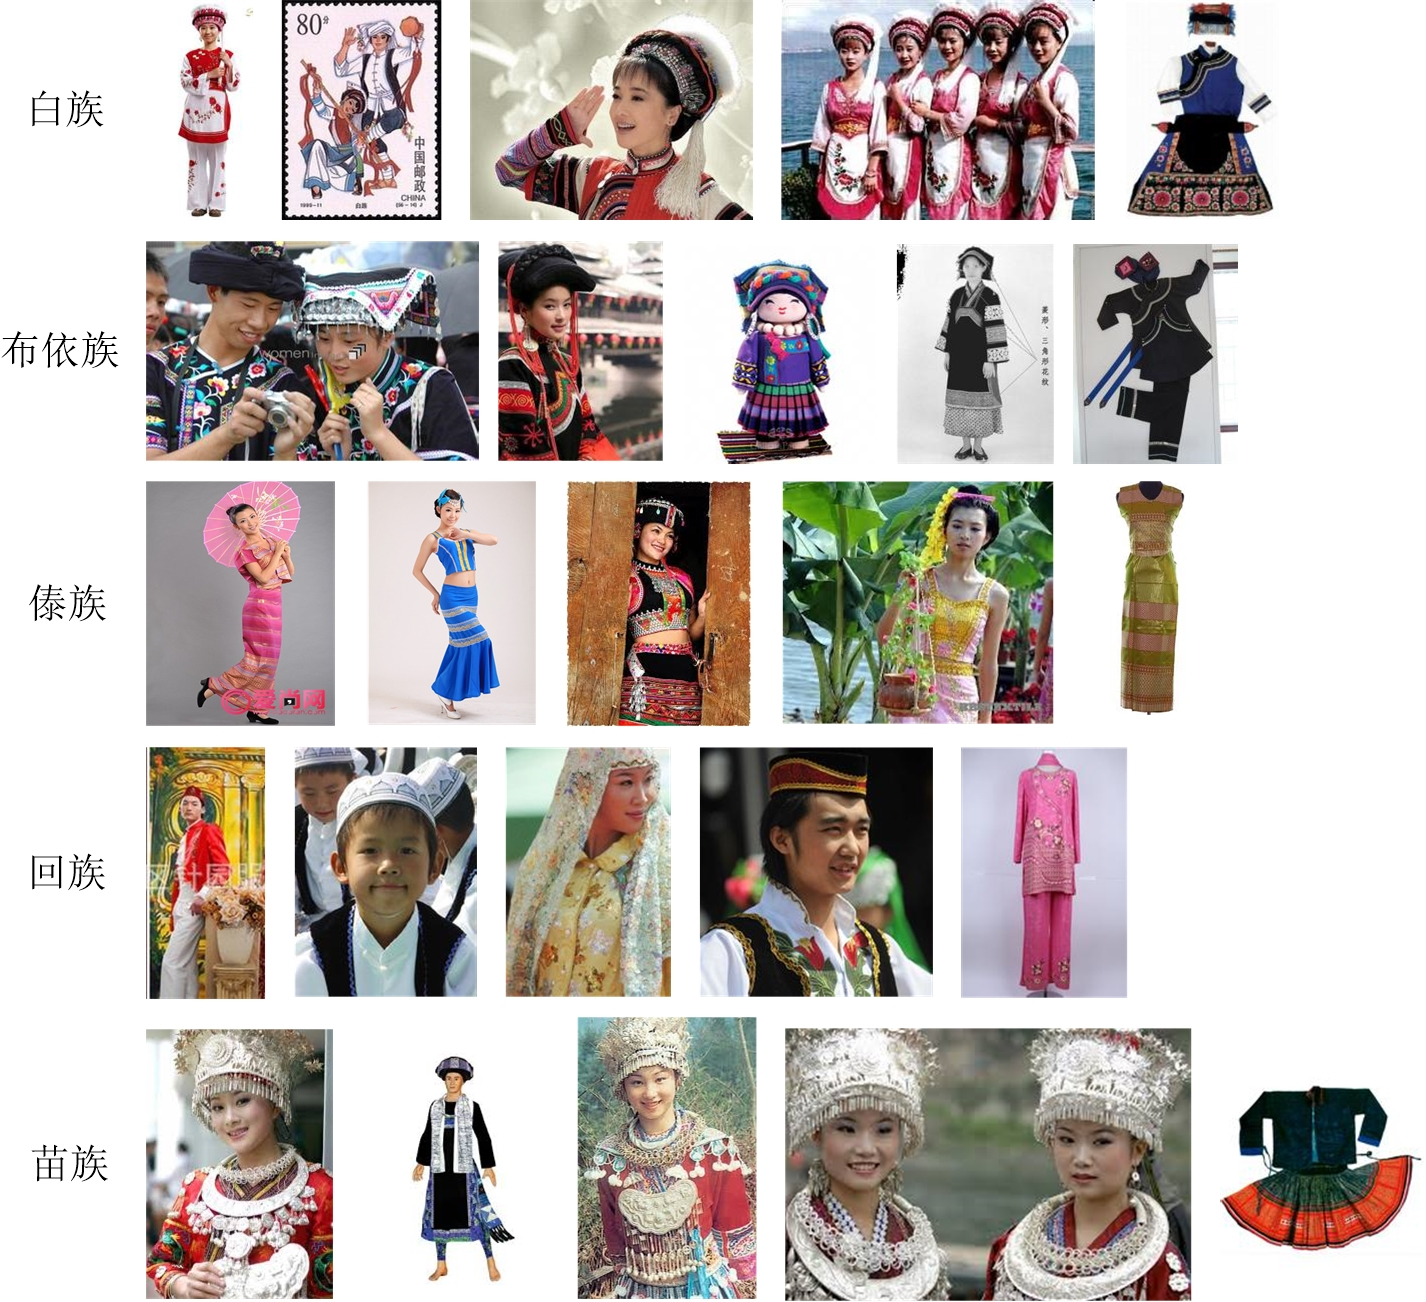
\includegraphics[width=1\textwidth]{costume-12.jpg}
	\caption{Costume-12数据集中的部分图片}\label{fig:costume-12}
\end{figure}

\subsubsection{Costume-38数据集}
Costume-38数据集包含38个中国少数民族,其图片来源于纪录片《中国少数民族》中的视频截图,因此图片中包含的服饰一定为相应民族的服饰,不会存在错误。由于每个民族的纪录片长度不同,所以得到的截图数量也不尽相同,多的有六十几张,少的只有二十张,共1342张图片。Costume-38数据集中绝大多数图片包含人,少部分图片只包含服饰、首饰等。图\ref{fig:costume-38}展示了Costume-38中的部分图片。

\begin{figure}
	\centering
	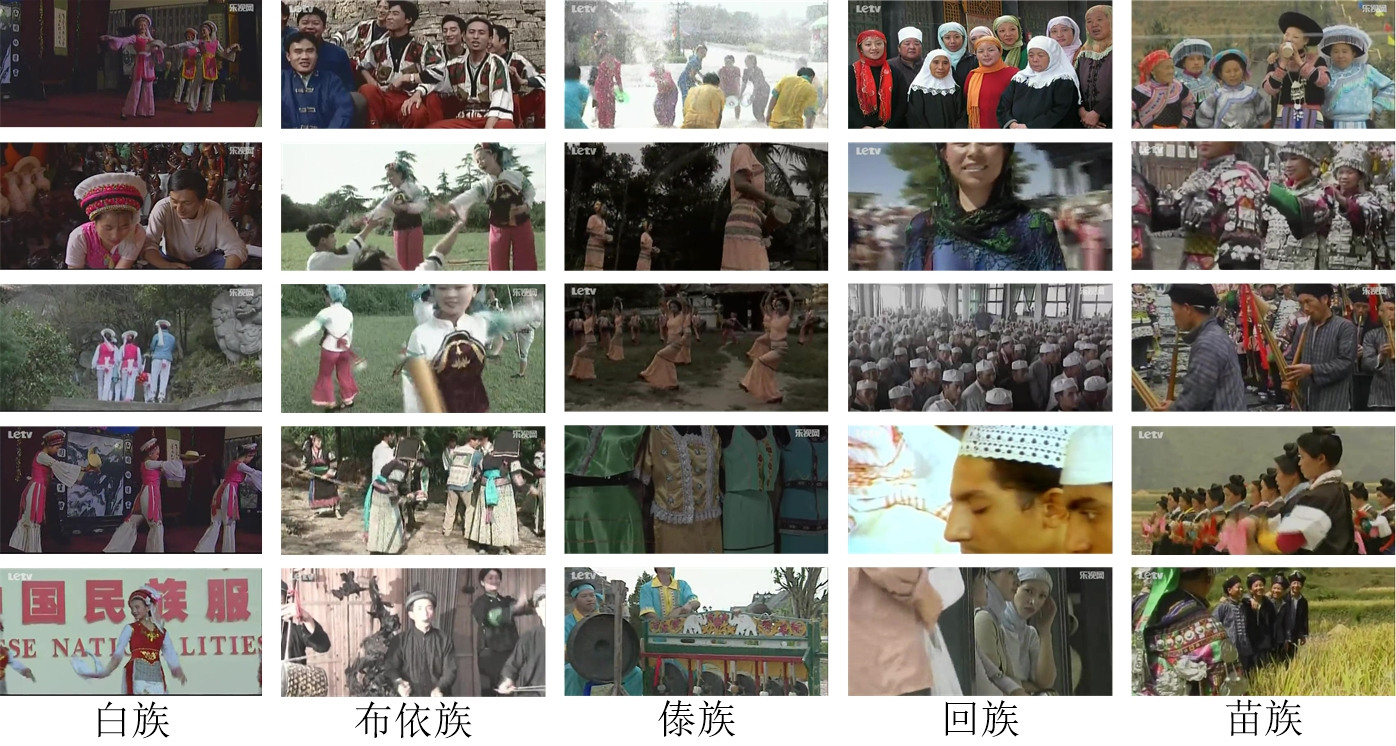
\includegraphics[width=1\textwidth]{costume-38.jpg}
	\caption{Costume-38数据集中的部分图片}\label{fig:costume-38}
\end{figure}

\subsubsection{实验流程与实验结果}

使用CostumeNet做服饰检测的流程与前面的MONet和使用CNN进行图像检索的思路类似,分为三个部分:
\begin{enumerate}
	\item 预处理:使用MONet判断图片的主方向;
	\item 训练和分类:使用预处理得到的图片训练VGG-19网络,并使用该网络对图片进行分类(Costume-12为12类,Costume-38为38类);
	\item 后处理:提取网络全连接层的输出作为图片的特征,使用SVM再进行分类。
\end{enumerate}

实验结果如表\ref{tab:costume}所示。其中第一列“SVM”表示使用VGG网络提取图片特征(不经过fine-tune)然后使用SVM分类的结果;第二列“VGG”表示使用VGG fine-tune的结果;第三列表示使用fine-tune的网络提取图片特征然后用SVM分类的结果;结果用准确率$R$表示($R=\frac{\#correct}{\#correct+\#false}$)。对于Costume-12数据集,每一类我们使用50张图片进行测试,其余图片进行训练;对于Costume-38数据集,每一类我们使用10张图片记性测试,其余图片进行训练。通过实验结果可以看出,直接使用未经过fine-tune的网络提取的特征做SVM效果并不理想,而使用fine-tune后的结果有较大的提升。使用“VGG+SVM”的策略,在Costume-12上可以达到95.3\%的准确率,在Costume-38上可以达到85.0\%的准确率,达到了较为理想的效果。并且在Costume-12数据集上,由于存在错误图片,准确率很难再有提升;而在Costume-38数据集上,每一类的图片数量有限,在后面的工作中,可以继续扩大数据集,提高准确率。
\begin{table}
	\begin{center}
		\begin{tabular}{|c|c|c|c|}
			\hline
			           & SVM & VGG & VGG+SVM \\
			\hline
			Costume-12 & 0.648 & 0.823 & 0.953\\
			\hline
			Costume-38 & 0.371 & 0.584 &0.850\\
			\hline
		\end{tabular}
	\end{center}
	\caption{CostumeNet实验结果}
	\label{tab:costume}
\end{table}

\subsubsection{Demo展示}
基于上述实验框架和模型,我们搭建了一个可以进行服饰检测的平台,其展示效果图\ref{fig:costume-demo}所示。
\begin{figure}
	\centering
	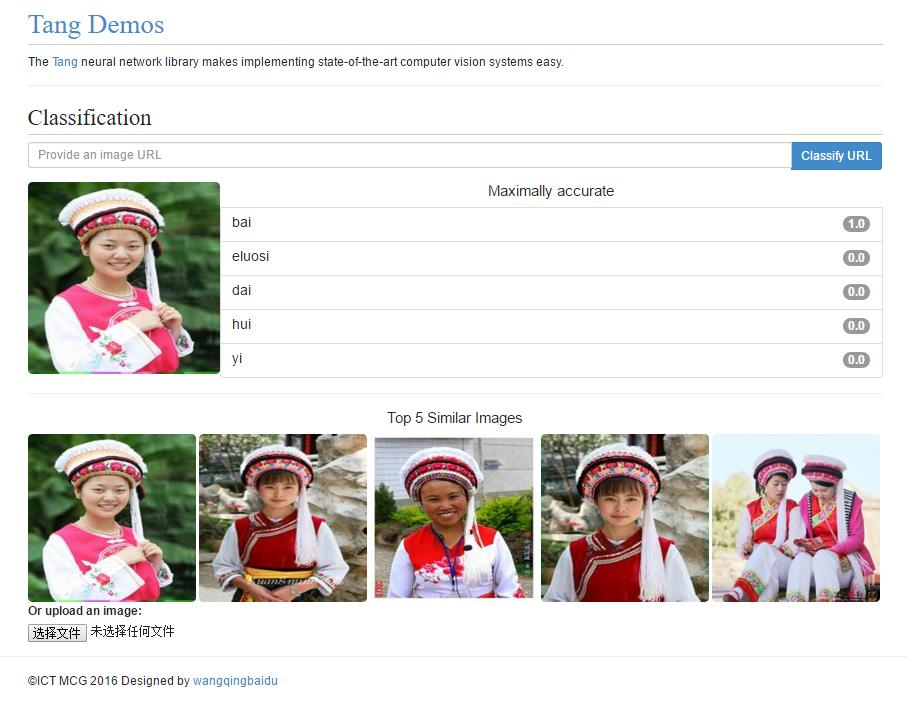
\includegraphics[width=1\textwidth]{cnndemo.jpg}
	\caption{服饰检测Demo展示}\label{fig:costume-demo}
\end{figure}


\section{本章小节}
在本章中,我们分析并证明了CNN图像检测框架中存在的一个问题:无法克服图片旋转带来的性能下降。我们也介绍了目前解决该问题的主流方法,包括数据扩大、Max Pooling特征融合等等,但是这些方法都有其局限性。通过分析以上问题,我们提出了MONet,其思想是通过学习的方向,训练出一个可以自动识别图片主方向的网络,并在进行图像检索之前通过MONet对图片记性预处理。在设计MONet时,我们考虑模型复杂度和训练、分类速度等问题,最终基于Inception思想设计出了MONet的网络结构。由于MONet是一个对图片的预处理步骤,所以可以简单地与现有的任何模型进行融合,本章也介绍了MONet的应用,包括将MONet应用于传统的基于BoW的检索框架和民族服饰检索任务。目前MONet也存在一些局限性,包括无法更加精细的判断图片的主方向;增加图像检索的预处理时间等。








%\chapter{总结与展望}
\section{研究工作总结}
信息化社会的到来,社交网络的用户量在爆发式增长。
社交网络中信息的扩散机制和基于社交网络的营销策略越发成为研究热点。
在本文中,我们研究学习了社交网络中一些非次模的问题,主要是基于非次模的阈值函数。
之前的研究大多集中在次模阈值函数和次模影响力函数,我们的研究和他们大不相同。
根据前人的实验观察,我们研究了两类非次模函数----$\varepsilon$-次模逼近函数和$k$-激活函数,
然后分别讨论了基于$\varepsilon$-次模逼近函数的影响力最大化问题和基于$k$-激活函数的小世界网络路由问题。
首先我们证明了尽管$\varepsilon$-次模逼近函数和次模函数很接近,
在有$\varepsilon$-次模逼近节点的图中影响力最大化问题依然很难近似。
通过构造概率与门并从NP完全问题集合覆盖归约,我们证明了
$n$个节点的图中只要有$n$的多项式个$\varepsilon$-次模逼近节点影响力最大化算法就无法做到$log$近似。
然后我们通过把$\varepsilon$-次模逼近函数替换成次模的上界或者下界,转化问一个次模优化问题,
设计了近似算法\textsf{Galg-U}和\textsf{Galg-L}。
基于概率空间映射,我们证明了这个近似算法的近似比为$(1-\frac{1}{e})(1-\varepsilon)^c$,
其中$c$是$\varepsilon$-次模逼近节点的个数。
接下来我们研究了Kleinberg小世界网络中,基于$k$-激活函数的路由。
本文定量地研究了从两个相邻的种子节点开始去感染一个网格上最远目标$t$需要的步数,也就是路由时间。
在每一步,只有一个节点会被激活,选择被激活节点的策略是分散式的,也就是路由选择策略只能基于当前被激活的节点发出的强连接和弱连接。
复杂路由比较像社交网站上最近提出的一个应用:主动交友,主动交友是指在像Facebook、人人网等社交网站上通过添加一些中间好友来增加目标接受自己好友请求的概率\cite{YangHLC13}。
本文指出与$k$-激活传播不同,对于所有的$\alpha$,$k$-激活路由时间均有$n$的多项式的下界,即使每一步允许激活多个节点。


本文的最后实现了算法\textsf{Galg-U}和\textsf{Galg-L}和其他基准算法,
并且在真实的社交网络{\em NetHEPT}、{\em Flixster}和{\em DBLP}上测试对比了算法和其他基准算法效果。
在小数据集上,\textsf{Galg-U}和\textsf{Galg-L}算法效果比\textsf{Greedy}稍好,
但是算法的运行时间要少很多,因为\textsf{Galg-U}和\textsf{Galg-L}可以利用一些次模上下界利用\textsf{TIM}算法加速。
在较大的网络{\em Flixster}和{\em DBLP}上,\textsf{Galg-U}和\textsf{Galg-L}均比其他基准算法要好。
而且在$\varepsilon$-次模逼近节点个数达到总结点个数$\frac{1}{3}$时,算法的表现依然很好。
这说明\textsf{Galg-U}和\textsf{Galg-L}不仅仅有理论近似比保证,实际中运行效果也很好。




\section{未来工作的展望}
在影响力最大化问题上,本文目前的研究主要集中在$\varepsilon$-次模逼近函数,
但是对于那些和次模函数相距很远的非次模阈值函数,我们还不知道如何设计有效的算法。
此外,我们提出的算法在实验中采用了逆向可达集合进行加速。
并不是所有的次模函数都可以使用逆向可达集合,
研究哪些函数可以使用逆向可达集合进行加速或者设计基于次模函数的加速算法也是新的研究方向。

其次,在研究$k$-激活路由时,为了更好地应用延迟选择原则,本文采用了有向Kleinberg小世界网络模型。
因为每个节点的弱连接平均数量仍为常数,有向小世界网络和无向小世界网络中$k$-激活路由的效率应该不会相差太多。
后续的工作希望可以研究$k$-激活路由在无向Kleinberg小世界网络中的性能。
未来也可以研究在什么样结构的网络中$k$-激活路由可以很快找到目标,探讨$k$-激活路由在其他小世界模型中的执行效率。
为$k$-激活路由寻找更广泛的应用场景也是未来需要进行的工作之一。



\ICTbackmatter{\bibliography{bib/ref}\nocite{*}}
%\bibliography{bib/ref}
%
\begin{thanks}


在完成硕士学位论文之际,我在此向所有支持我、关心我的老师、师兄、同学和家人致以最衷心的感谢。
是你们的帮助,让我能够顺利完成毕业设计。
感谢中科院计算所前瞻实验室所对我的支持,感谢算法与复杂性课题组,
让我能够在一个科研环境优越的地方研究学习。


首先十分感谢我的指导教师孙晓明研究员。
自从我研一进入实验室以来,孙老师在科研、学习、生活方面给了我非常多的帮助。
感谢孙老师对我论文的选题、设计、完成以及论文修改等各个方面给予的悉心指导。
我也要感谢答辩组的各位老师,卜东波老师、和张家琳老师,你们在开题答辩和中期检查时都给提出了我非常重要的指导意见,
让我对自己的工作有了更深刻的认识,得到了新的启示。

我还要感谢在微软亚洲研究院实习时对我科研进行过指导的陈卫老师,
每周和你的讨论我都收益颇多,你对我在科研部分给予了细致的指导,在这里衷心地感谢你对我的教导。


感谢我的好朋友曾钢同学,毕设过程中我们互相鼓励,谢谢你的一路支持。
也感谢我的舍友顾茂杰和朱良昌以及实验室的岑武斌同学,是你们陪伴我走过了毕设的日子,谢谢你们对我的鼓励和支持。
我还要感谢实验室的师兄师姐们,感谢你们对我毕业设计提出了宝贵的意见,耐心的解答我们的疑惑。

在此,也要感谢我的家人对我的支持和鼓励,特别是父亲和母亲,你们的鼓励永远让我充满动力。

最后要感谢我的女朋友,在研究生阶段,让我踏实安心的工作,默默地支持我,谢谢你一直以来的陪伴!


感谢所有给予过我帮助与支持的老师同学们!


\end{thanks}

%
\begin{resume}

\begin{resumelist*}{教育经历}
\resumelistitem 2009年9月---~2013年7月,武汉大学,计算机学院,学士
\resumelistitem 2013年9月---~2016年7月,中国科学院,计算技术研究所,硕士
\end{resumelist*}

\begin{resumelist}{【攻读硕士学位期间发表的论文】}
\resumelistitem Jingya Tang, Dongming Zhang, Yongdong Zhang, Qi Tian, Region Similarity Arrangement for Image Retrieval. IEEE International Conference on Multimedia and Expo (ICME), IEEE, 2016. 
\end{resumelist}

\begin{resumelist}{【攻读硕士学位期间参加的科研项目】}

\resumelistitem 大规模图像检索系统(国家高新技术研究与发展计划)
\resumelistitem 基于区域相似性的大规模图像检索的研究 
\resumelistitem 基于深度卷积网络的民族服饰检测的研究

\end{resumelist}

\end{resume}

\end{document}
